%This template was prepared by Dorothea F. Brosius of the
%Institute for Electronics and Applied Physics, University of Maryland, College Park, MD
%The template was last updated in January 2019
%Thesis Main Page used with thesis.sty is based on the latest version of the 
%University of Maryland Electronic Thesis and Dissertation (ETD) Style Guide (2017)
% August 2017 (TOC contents linked in blue in pdf file)
%The YourInformation file was created by Freja Nordsiek, 2014.
%Code for linking the TOC titles to the text in the pdf file was created by Freja Nordsiek, 2014.

% Select the version that fits how you are making this LaTeX document (its driver).
% The first two are the most likely ones to be needed.

 \newcommand{\mydriver}{pdflatex} %Making a PDF directly using pdflatex.
%\newcommand{\mydriver}{dvipdfmx} %Making a DVI and converting that to PDF using dvipdfmx.
%\newcommand{\mydriver}{dvipdfm} %Making a DVI and converting that to PDF using dvipdfm.
%\newcommand{\mydriver}{dvips} %Making a DVI and converting that to PS using dvips (may later be converted to PDF).
%\newcommand{\mydriver}{dvipsone} %Making a DVI and converting that to PS using dvipsone (may later be converted to PDF).
%\newcommand{\mydriver}{ps2pdf} %Same as the one for dvips except it is compatible with Ghostscript's PDF writer.


\documentclass[12pt,\mydriver]{thesis}  %12pt is larger than 11pt

\usepackage{titlesec}
   \titleformat{\chapter}
      {\normalfont\large}{Chapter \thechapter:}{1em}{}
\usepackage{graphicx}
\usepackage{cite}
\usepackage{lscape}
\usepackage{indentfirst}
\usepackage{latexsym}
\usepackage{multirow}
\usepackage{epstopdf}
\usepackage{tabls}
\usepackage{wrapfig}
\usepackage{slashbox}
\usepackage{longtable}
\usepackage{supertabular}
%\usepackage{subeqn}
\usepackage{subfigure}
\usepackage{floatrow}
\usepackage{amsmath}
\usepackage{amssymb}
\usepackage{dsfont}
\usepackage{physics}
%\usepackage{natbib}  % To be used with Natbib

%hyperref
\usepackage[colorlinks=true,urlcolor=black,linkcolor=blue,citecolor=blue]{hyperref}

%Ian's macros
\def\ex{\mathbf{e}_x}  
\def\ey{\mathbf{e}_y}  
\def\ez{\mathbf{e}_z}  

\def\kr{k_{\rm R}}                            				
\def\vr{v_{\rm R}}                            				
\def\Er{E_{\rm R}} 
\def\lambdar{\lambda_{\rm R}} 
\def\Or{\Omega_{\rm R}}
\def\Hr{H_{\rm R}}


\newcommand{\tbsp}{\rule{0pt}{18pt}} %used to get a vertical distance after \hline
\renewcommand{\baselinestretch}{2}
\setlength{\textwidth}{5.9in}
\setlength{\textheight}{9in}
\setlength{\topmargin}{-.50in}
%\setlength{\topmargin}{0in}    %use this setting if the printer makes the the top margin 1/2 inch instead of 1 inch
\setlength{\oddsidemargin}{.55in}
\setlength{\parindent}{.4in}
\pagestyle{empty}

\begin{document}
\pagestyle{empty}
%Abstract Page

\hbox{\ }

\renewcommand{\baselinestretch}{1}
\small \normalsize

\begin{center}
\large{{ABSTRACT}}

\vspace{3em}

\end{center}
\hspace{-.15in}
\begin{tabular}{ll}
Title of dissertation:   & {\large  ANDERSON LOCALIZATION IN PRESENCE OF }\\
&                     {\large  SPIN-ORBIT COUPLING IN AN ATOMIC} \\
&                     {\large  BOSE GAS} \\
\ \\
&                          {\large  Yuchen Yue} \\
&                           {\large Doctor of Philosophy, 2019} \\
\ \\
Dissertation directed by: & {\large  Professor Ian Spielman} \\
&               {\large  Joint Quantum Institute,}\\
&               {\large National Institute of Standards and Technology}\\
&               {\large and the University of Maryland} \\
\end{tabular}

\vspace{3em}

\renewcommand{\baselinestretch}{2}
\large \normalsize

abstract
 %(must be first, required, non-numbered)
%Titlepage

\thispagestyle{empty}
\hbox{\ }
\vspace{1in}
\renewcommand{\baselinestretch}{1}
\small\normalsize
\begin{center}

\large{{ANDERSON LOCALIZATION IN PRESENCE OF SPIN-ORBIT \\
COUPLING IN AN ATOMIC BOSE GAS}}\\
\ \\
\ \\
\large{by} \\
\ \\
\large{Yuchen Yue}%Your full name as it appears in University records.
\ \\
\ \\
\ \\
\ \\
\normalsize
Dissertation submitted to the Faculty of the Graduate School of the \\
University of Maryland, College Park in partial fulfillment \\
of the requirements for the degree of \\
Doctor of Philosophy \\
2019
\end{center}

\vspace{7.5em}

\noindent Advisory Committee: \\
Professor Rajarshi Roy, Chair/Advisor \\
Dr. Parvez N. Guzdar, Co-Advisor \\
Professor Robert W. Gammon \\
Professor Thomas Antonsen \\
Professor Edward Ott
 %(must follow Abstract, required, non-numbered)
\include{Copyright} %(highly recommended, non-numbered)

%Pages from this point start at lower-case Roman number ii)
\pagestyle{plain} \pagenumbering{roman} \setcounter{page}{2}
\addcontentsline{toc}{chapter}{Preface}
\include{Preface}  %(if present, start at lower-case Roman number ii)
\addcontentsline{toc}{chapter}{Foreword}
\include{Foreword} %(if present, lower-case Roman)
\addcontentsline{toc}{chapter}{Dedication}
%Dedication

\renewcommand{\baselinestretch}{2}
\small\normalsize
\hbox{\ }
 
\vspace{-.65in}

\begin{center}
$To~my~parents~and~grandparents$
\end{center} 


 %(if present, lower-case Roman)
\addcontentsline{toc}{chapter}{Acknowledgements}
%Acknowledgments

\renewcommand{\baselinestretch}{2}
\small\normalsize
\hbox{\ }
 
\vspace{-.65in}

\begin{center}
\large{Acknowledgments} 
\end{center} 

\vspace{1ex}

First of all, I would like to thank my parents and grandparents for everything they have done for me, and their love and support. I began to realize how important they are and how much I miss them after I studied in a foreign country for years. 

Next, I would like to thank my Ph.D. advisor, Dr. Ian Spielman. Ian has been a great advisor. He is always patient in our discussions and always tries to explain physics most intuitively. He would draw nice sketches on the whiteboard which helps him explaining his idea. He would also come to the lab and dig into the hardware together with us and find out why something is not working. When I first joined the group, I had a hard time understanding him because he speaks extremely fast. Over the years, I got much better in communication and I learned a lot from him, not just physics, but also being optimistic when facing uncertainties and difficulties.

During the years, I worked with other members of the RbChip lab. Seiji Sugawa, Francisco Salces-C\'arcoba, Andika Putra, Christopher Billington, and Emine Altuntas, thank you for making RbChip lab an enjoyable place to work. I miss the old times when we can have lunch together, especially after being quarantined at home for half a year in the Covid-19 pandemic.

Lastly, I would like to thank my girlfriend, Dr. Yuchen Yang, who also got her Ph.D. in 2020. We are together nearly the entire time of our Ph.D., we share not only our first name in English but our values of life. I'm very lucky to meet you. 
 %(if present, lower-case Roman)
    \cleardoublepage
    \phantomsection
    \addcontentsline{toc}{chapter}{Table of Contents}
    \renewcommand{\contentsname}{Table of Contents}
\renewcommand{\baselinestretch}{1}
\small\normalsize
\tableofcontents %(required, lower-case Roman)
\newpage
\listoftables %(if present, lower-case Roman)
\newpage
\listoffigures %(if present, lower-case Roman)
\newpage
% LIST OF ABBREVIATIONS
\addcontentsline{toc}{chapter}{List of Abbreviations}
%List of Abbreviations


\renewcommand{\baselinestretch}{1}
\small\normalsize
\hbox{\ }

\vspace{-4em}

\begin{center}
\large{List of Abbreviations}
\end{center} 

\vspace{3pt}

\begin{supertabular}{ll}
AAA & Antiaircraft artillery \\

%$\alpha$ & alpha \\
%$\beta$  & beta \\
%&  \\ 
%IREAP & Institute for Research in Electronics and Applied Physics \\
%NSA & National Security Agency
\end{supertabular}


\newpage
\setlength{\parskip}{0em}
\renewcommand{\baselinestretch}{2}
\small\normalsize

%Pages from this point start at Arabic numeral 1
\setcounter{page}{1}
\pagenumbering{arabic}
%Chapter 1

\renewcommand{\thechapter}{1}

\chapter{Theoretical description of Bose-Einstein condensate}

This chapter starts from the difference in description of particles between classical mechanics and quantum mechanics, indistinguish-ability and exclusion of identical particles lead to dramatically different statistical properties. More fundamentally, I include some discussion about exchange symmetry and why it is related to particle's spin. Next is the fine structure and hyperfine structure of an atom, atom-light interaction. After that, Laser cooling techniques are introduced followed by many-body description of BEC.   
\section{Bose-Einstein statistics}
\subsection{Classical description of particles}
Classical mechanics originate from Newtonian mechanics and have different but equivalent formulations. It assumes the position and velocity of an object can be measured and kept track of at any time. The dynamics of an object or a system of objects can be sufficiently described by their positions and velocities. For example, in one of the equivalent formulations, Hamiltonian mechanics \cite{goldstein2002classical}, a classical system is described by a set of canonical coordinates $\vec{r} = (\vec{p},\vec{q})$. Here $\vec{p} = (p_1,p_2,\cdots,p_N)$  and $\vec{q}= (q_1,q_2,\cdots,q_N)$, they are indexed by the N-dimensional frame of reference of the system. Hamiltonian $\mathcal{H} = \mathcal{H}(\vec{p},\vec{q},t)$ is a function of canonical coordinates and corresponds to total energy of a system. The dynamics of the system is governed by equations
\begin{equation}\label{cla ham}
\begin{aligned}
    &\frac{d\vec{p}}{dt} = -\frac{\partial\mathcal{H}}{\partial\vec{q}}\\
   &\frac{d\vec{q}}{dt} = \frac{\partial\mathcal{H}}{\partial\vec{p}}
\end{aligned}
\end{equation}
Both $\vec{p}$ and $\vec{q}$ evolve with equation \ref{cla ham} deterministically and for a system of classical particles, each particle's trajectory can be traced during evolution, making them distinguishable from each other.

In classical statistical mechanics, the Maxwell-Boltzmann statistics describes the distribution of non-interacting particles in thermal equilibrium over energy states. The ensemble averaged number of particles in energy state $\epsilon_i$ is
\begin{equation}
    n_i = \frac{g_i}{\exp{(\epsilon_i-\mu)/k_BT}}.
\end{equation}
Here, $g_i$ is the degeneracy of energy state $\epsilon_i$, $\mu$ is the chemical potential which can be obtained from the conservation of particle number. $k_B$ is the Boltzmann's constant and $T$ is temperature.  
\subsection{Quantum description of particles}
Quantum mechanics, formed by six postulates, is very powerful in explaining modern experiments in atomic, molecular, optical and condensed matter physics and so on. It also introduces counter-intuitive concepts such as photon, matter wave and Pauli's exclusion principle. These concepts won't be well understood without a good sense of the postulates which are listed in appendix \ref{appendix:QMP}.  

As the first postulate states, a particle is described by its quantum state $\ket{\Psi(t)}$. $\ket{\Psi(t)}$ contains all the information about the particle and can be represented by projecting it in any complete basis. For example, $\Psi(\mathbf{r},t) = \bra{\mathbf{r}}\ket{\Psi(t)}$ is defined as the spatial wave function of the particle. Since $\ket{\mathbf{r}}s$ form a complete basis, wave function $\Psi(\mathbf{r},t)$ is sufficient to represent state $\ket{\Psi(t)}$. Similarly, projecting $\Psi(t)$ in k space, we can define wave function in momentum space $\Psi(\mathbf{p},t) = \bra{\mathbf{p}}\ket{\Psi(t)}$. As postulate four states, for a particle in state $\Psi(t)$, without measurement, the only information available to us is the probability of the particle being in position $\mathbf{r}$ and momentum $\mathbf{p}$, it is not possible to know the position and momentum of the particle without measurement. Moreover, as postulate five states, immediately after the measurement of an observable, the state collapse to one of its eigenstates, meaning after a measurement, the particle's state will be changed. 
\subsection{Distinguishability}
For a group of identical particles, their spatial state can overlap at any time, and when they do, the lack of information and inability to do measurements without changing their states make it in principle impossible to track the particles.  And thus, in quantum mechanics, identical particles are indistinguishable. This indistinguishability has a fundamental effect on the statistics of particles.

\subsection{Exchange symmetry of identical particles}

For a group of identical particles, the many-body state describing the system should not have any measurable difference exchanging any two particles of them. In quantum mechanics, a state is determined up to a phase factor. For a state $\ket{\Psi(t)}$, $e^{i\theta}\ket{\Psi(t)}$ does not have any measurable difference for any $\theta \in \mathbb{R}$. So for a two-particle state $\ket{\psi_1\psi_2}$, exchange the two particles, in the most general case, the two-particle state should become $e^{i\theta}\ket{\psi_2\psi_1}$. People may argue that exchanging particles twice the state should return, $e^{i2\theta} = 1$, but it is not rigorous. It was introduced as symmetry postulate that $e^{i\theta}$ can only take the value of $+1$ or $-1$, meaning the two-particle state can only be symmetric or anti-symmetric. It has deep consequences in particle statistics and is in good agreement with experimental facts. However, its theoretical justification remains unclear. In 1977, J.M.Leinass and J.Myrheim introduced in their paper \cite{leinaas1977theory} a quantization formalism, in which the restriction on wave function to be either symmetric or antisymmetric appears in a natural way, without having to add any additional constraints. However, this is true only when space is at least three-dimensional. In one or two dimensions, $e^{i\theta}$ can take other values. Frank Wilczek invented the term "anyon" to describe this kind of particle and they are important in understanding the fractional quantum Hall effect.   


\subsection{Bosons, Fermions and spin statistics}
In three dimensional space, particles' wave function can only be symmetric or anti-symmetric. The symmetry of the wave function is determined by the particles' spin. A particle is called Boson if it has an integer spin and Fermion if it has a half-integer spin. In consequence, the wave functions of Bosons and Fermions are symmetric and anti-symmetric, respectively.  The spin statistics theorem is first formulated in 1939 by Markus Fierz\cite{fierz1939relativistische} and rederived in a more systematic way in 1940 by Wolfgang Pauli\cite{pauli1940connection}. A more conceptual argument was provided in 1950 by Julian Schwinger. It is fascinating and very non-intuitive how particles' spin determines their exchange symmetry. As Feynman commented in his book \textit{Feynman Lectures on Physics}\cite{feynman2011feynman}: \textit{An explanation has been worked out by Pauli from complicated arguments of QFT and relativity. But we have not found a way of reproducing his arguments on an elementary level. This probably means that we do not have a complete understanding of the fundamental principle involved.}
  
\subsection{Bose-Einstein statistics and non-interacting BEC}
Quantum statistics differs from classical statistics in two aspects, indistinguishability and exchange symmetry. 

For a two-particle wave function $\psi(\mathbf{r}_1,\mathbf{r}_2)$, if the two particles are Fermions, they can not occupy the same state. $\psi(\mathbf{r}_1,\mathbf{r}_2) = -\psi(\mathbf{r}_2,\mathbf{r}_1)$, if $\psi(\mathbf{r}_1,\mathbf{r}_2) = \psi(\mathbf{r}_2,\mathbf{r}_1)$, $\psi(\mathbf{r}_1,\mathbf{r}_2) = 0$. For Bosons, this is not the case. Any number of Bosons can occupy the same state and the system has the lowest energy when all the Bosons are in the ground state.

The Bose-Einstein distribution can be derived from the principle of maximum entropy. A Boson system with $N$ particles are distributed to states $\{\ket{\epsilon_i}\}$, each state $\ket{\epsilon_i}$ has degeneracy $g_i$ and it is occupied by $n_i$ particles. The number of micro-state is
\begin{equation}
    \Omega(\{n_i\}) = \prod_{i} \frac{(n_i+g_i-1)!}{n_i!(g_i-1)!}.
\end{equation}
Maximizing $\Omega(\{n_i\})$ under the constraints $\sum_{i}n_i = N$ and $\sum_{i}n_i\epsilon_i = U$, we can derive Bose-Einstein distribution
\begin{equation}
    n_i = \frac{1}{\exp{-\alpha-\beta\epsilon_i}-1},
\end{equation}
$\alpha$ and $\beta$ are the Lagrange multipliers. From constraints $\sum_{i}n_i = N$ and $\sum_{i}n_i\epsilon_i = U$, it can be determined $\alpha$ is chemical potential $\mu$ over $k_BT$ and $\beta$ is $-1/k_BT$ where $k_B$ is Boltzmann constant and $T$ is temperature.

To find out how does this distribution lead to Bose-Einstein condensates, we need to revisit the constraints. For a system of particles in a box of volume V. The energy density of states is
\begin{equation}
    g(\epsilon) = \frac{V}{4\pi^2}\big(\frac{2m}{\hbar}\big)^{3/2}\sqrt{\epsilon}    
\end{equation}
Replacing the sum in $\sum_{i}n_i = N$ with integral, we get
\begin{equation}\label{N}
    \frac{V}{4\pi^2}\big(\frac{2m}{\hbar}\big)^{3/2}\int_0^\infty\frac{\sqrt{\epsilon}}{\exp{(\epsilon-\mu)/k_BT}-1}d\epsilon = N
\end{equation}
Denote the integral as $I(\mu)$
\begin{equation}
    I(\mu) = \int_0^\infty\frac{\sqrt{\epsilon}}{\exp{(\epsilon-\mu)/k_BT}-1}d\epsilon
\end{equation}
For Eq.~(\ref{N}) to hold, $I(\mu)$ should be a constant, and $\mu$ should be a function of $T$. As $T$ decreases, $\mu$ should increase to keep $I(\mu)$ constant. But $\mu$ can not go positive because in that case, for states $\epsilon_i-\mu < 0$, $n_i$ will be negative. So as $T$ decreases to some critical temperature $T_c$, $\mu$ increases to 0 to keep $I(\mu)$ constant. As $T$ continue decreasing, $\mu$ can not increase anymore and we have
\begin{equation}
    \frac{V}{4\pi^2}\big(\frac{2m}{\hbar}\big)^{3/2}\int_0^\infty\frac{\sqrt{\epsilon}}{\exp{(\epsilon-\mu)/k_BT}-1}d\epsilon < N
\end{equation}
Where are the missing particles? The answer is they are condensed in the ground state with zero energy. If we look at the density of state $g(\epsilon)$, it is zero for the ground state. When $T$ is high, the number of particles that are in the ground state is negligible, so the integral counts all the particles and equals $N$. When $T<T_c$, $\mu$ is zero, a significant amount of particles start to occupy the ground state, and the missed particles will cause the loss of atoms counts. 

The critical temperature can be calculated from Eq.~(\ref{N}) with $\mu=0$.
\begin{equation}
    T_c = \frac{2\pi\hbar^2}{mk_B}\Big(\frac{N}{\eta(3/2)V}\Big)^{2/3}
\end{equation}
where $\eta(x)$ is Riemann zeta function. And it can be shown the fraction of particles in the ground state is a function of $T$ and $T_c$
\begin{equation}
    \frac{N_0}{N} = 1-\Big(\frac{T}{T_c}\Big)^{3/2}.
\end{equation}






\section{Manybody BEC system}\label{sec MB}
\subsection{Second quantization}
An interacting system can be described by the second quantization Hamiltonian. In the second quantization framework, particles in a system are described by creation and annihilation operators on the basis of many-body Fock states. Creation operators $\hat{a}_k^\dag$ creates a particle in the Fock state $\ket{n_1,\dots , n_k,\dots}$ while annihilation operators $\hat{a}_k$ annihilates a particle in the Fock state $\ket{n_1,\dots , n_k,\dots}$.  
\begin{equation}
\begin{aligned}
    &\hat{a}_k^\dag\ket{n_1,\dots , n_k,\dots} = \sqrt{n_k+1}\ket{n_1,\dots,n_k+1,\dots}\\
    &\hat{a}_k\ket{n_1,\dots,n_k,\dots} = \sqrt{n_k}\ket{n_1,\dots,n_k-1,\dots}
\end{aligned}
\end{equation}
With a change of basis, the spatial creation and annihilation operators can be defined as
\begin{equation}
    \begin{aligned}
    &\hat{\psi}(\Vec{r}) = \sum_k \hat{a}_k \braket{\Vec{r}}{\Vec{k}} = \sum_k \hat{a}_k \frac{\exp{i\Vec{k}\cdot\Vec{r}}}{\sqrt{V}}\\
    &\hat{\psi}^\dag(\Vec{r}) = \sum_k \hat{a}^\dag_k \braket{\Vec{r}}{\Vec{k}} = \sum_k \hat{a}_k^\dag \frac{\exp{-i\Vec{k}\cdot\Vec{r}}}{\sqrt{V}}.\\
    \end{aligned}
\end{equation}
$\hat{\psi}^\dag(\Vec{r})$ and $\hat{\psi}(\Vec{r})$ creates and annihilates a particle at spatial coordinate $\Vec{r}$. Operator $\hat{N}_k = \hat{a}_k^\dag\hat{a}_k$ counts the number of particles in the momentum state $\ket{k}$. The two-particle operator is defined as 
\begin{equation}
    \begin{aligned}
    \hat{V}_{int} &= \frac{1}{2} \sum_{i\neq j}\hat{N}_i\hat{N}_j V_{ij} + \frac{1}{2}\sum_i \hat{N}_i(\hat{N}_i-1)V_{ii}\\
    & = \frac{1}{2}\sum_{i, j}(\hat{N}_i\hat{N}_j - \hat{N}_i\delta_{ij})V_{ij}
    \end{aligned}
\end{equation}
where $V_{ij}$ is the interaction between particles in states $\ket{i}$ and $\ket{j}$. From the orthogonality of Fock states and Pauli's exclusion principle, we can derive the commutators of creation and annihilation operators for both Bosons and Fermions.
For Bosons,
\begin{equation}
    \begin{aligned}
    &[\hat{a}_i, \hat{a}_j^\dag] = \delta_{ij}\\
    &[\hat{a}_i, \hat{a}_j] = [\hat{a}_i^\dag, \hat{a}_j^\dag] = 0
    \end{aligned}
\end{equation}
where $[A,B] = AB - BA$ is the commutator of operators $A$ and $B$.
For Fermions,
\begin{equation}
    \begin{aligned}
    &\{\hat{a}_i, \hat{a}_j^\dag\} = \delta_{ij}\\
    &\{\hat{a}_i, \hat{a}_j\} = \{\hat{a}_i^\dag, \hat{a}_j^\dag\} = 0
    \end{aligned}
\end{equation}
where $\{A,B\} = AB + BA$ is the anti-commutator of operators $A$ and $B$. With the change of basis, we can also obtain the commutation and anti-commutation relations of field operators $\hat{\psi}(\Vec{r})$ and $\hat{\psi}^\dag(\Vec{r})$.
For Bosons,
\begin{equation}
    \begin{aligned}
    &[\hat{\psi}(\Vec{r}~'), \hat{\psi}^\dag(\Vec{r}~'')] = \delta^3(\Vec{r}~'-\Vec{r}~'')\\
    &[\hat{\psi}(\Vec{r}~'), \hat{\psi}(\Vec{r}~'')] = [\hat{\psi}^\dag(\Vec{r}~'), \hat{\psi}^\dag(\Vec{r}~'')] = 0.
    \end{aligned}
\end{equation}
For Fermions,
\begin{equation}
    \begin{aligned}
    &\{\hat{\psi}(\Vec{r}~'), \hat{\psi}^\dag(\Vec{r}~'')\} = \delta^3(\Vec{r}~'-\Vec{r}~'')\\
    &\{\hat{\psi}(\Vec{r}~'), \hat{\psi}(\Vec{r}~'')\} = \{\hat{\psi}^\dag(\Vec{r}~'), \hat{\psi}^\dag(\Vec{r}~'')\} = 0.
    \end{aligned}
\end{equation}
With the commutators, we can rewrite the interaction operator $\hat{V}$,
\begin{equation}
    \hat{V}_{int} = \frac{1}{2}\sum_{i,j}\hat{a}_i^\dag\hat{a}_j^\dag V_{ij} \hat{a}_j\hat{a}_i,
\end{equation}
which is valid for both Bosons and Fermions.

In general, the Hamiltonian of a system is
\begin{equation}
    \hat{H} = \sum_i \frac{\hat{\textbf{p}}_i^2}{2m} + \hat{V}(\hat{\textbf{r}}_i) + \hat{V}_{int},
\end{equation}
in the representation of field operators, it takes the form
\begin{align}
    \hat{H} = &\int d\textbf{r} \hat{\Psi}^\dag(\textbf{r})\Bigg[-\frac{\hbar^2}{2m}\grad^2 + \hat{V}(\textbf{r})\bigg]\hat{\Psi}(\textbf{r})\\
    & + \frac{1}{2}\int d\textbf{r}'d\textbf{r}''d\textbf{r}'''d\textbf{r}''''\hat{\Psi}^\dag(\textbf{r}')\hat{\Psi}^\dag(\textbf{r}'')\matrixel{\textbf{r}'\textbf{r}''}{\hat{V}_{int}}{\textbf{r}'''\textbf{r}''''}\hat{\Psi}(\textbf{r}''')\hat{\Psi}(\textbf{r}'''')
\end{align}



\subsection{GPE of scalar BEC}
For dilute and cold gases, it is proper to approximate the interactions between atoms with two-body collisions. At low energy, the two-body collision interactions can be represented by the s-wave pseudopotential which is characterized by s-wave scattering length.
\begin{equation}
    \hat{V}_{int} = g\delta(\textbf{r}' - \textbf{r}''), 
\end{equation}
the constant $g$ is a function of scattering length $a$,
\begin{equation}
    g = \frac{4\pi\hbar^2a}{m}.
\end{equation}

The Hamiltonian of the cold gases system takes the form
\begin{align}
    \hat{H} = &\int d\textbf{r} \hat{\Psi}^\dag(\textbf{r})\left[-\frac{\hbar^2}{2m}\grad^2 + \hat{V}(\textbf{r})\right]\hat{\Psi}(\textbf{r})\\ \nonumber
    & + \frac{g}{2}\int d\textbf{r}\hat{\Psi}^\dag(\textbf{r})\hat{\Psi}^\dag(\textbf{r})\hat{\Psi}(\textbf{r})\hat{\Psi}(\textbf{r}),
\end{align}
and the dynamics of the field operators obey Heisenberg equation
\begin{align}
    i\hbar\frac{\partial}{\partial t}\hat{\Psi}(\textbf{r},t) &= \left[ \hat{\Psi}, \hat{H}\right]\\\nonumber
    &=\left[-\frac{\hbar^2}{2m}\grad^2 + \hat{V}(\textbf{r}) + g\hat{\Psi}^\dag(\textbf{r},t)\hat{\Psi}(\textbf{r},t) \right] \hat{\Psi}(\textbf{r},t)
\end{align}

Bogoliubov formulated the mean-field approach \cite{Bogolyubov:1947zz} to solving the cold dilute gases system by expanding the field operators to the first order,
\begin{equation}
    \hat{\Psi}(\textbf{r},t) = \Psi(\textbf{r},t) + \delta \hat{\Psi}(\textbf{r},t)
\end{equation}
$\Psi(\textbf{r},t)$ is the mean-field, the expectation value of field operator $\hat{\Psi}(\textbf{r},t)$, $\Psi(\textbf{r},t) = \expval{\hat{\Psi}(\textbf{r},t)}$. And $\delta \hat{\Psi}(\textbf{r},t)$ is the excitation term which describes the variation of the field operator around its expectation value. $\Psi(\textbf{r},t)$ is a classical field and is often called the wave function of the condensate. When excitation is small and can be neglected, we arrive at the dynamics of the classical field
\begin{equation}
    i\hbar\frac{\partial}{\partial t}\Psi(\textbf{r},t) =\left[-\frac{\hbar^2}{2m}\grad^2 + V(\textbf{r}) + g|\Psi(\textbf{r},t)|^2 \right]\Psi(\textbf{r},t)
\end{equation}

This equation is known as the Gross-Pitaevskii equation (GPE) which is derived by Gross \cite{gross1961structure} and Pitaevskii \cite{pitaevskii1961vortex} independently.

To obtain the ground state of the condensate, we can write the function $\Psi(\textbf{r},t)$ as $\Psi(\textbf{r},t) = \psi(\textbf{r})e^{-i\mu t/\hbar}$. Then the GPE becomes
\begin{equation}
    \mu \psi(\textbf{r}) =\left[-\frac{\hbar^2}{2m}\grad^2 + V(\textbf{r}) + g|\psi(\textbf{r})|^2 \right]\psi(\textbf{r})
\end{equation}
$\mu$ is chemical potential and is subject to the conservation of particle numbers
\begin{equation}
    \int d\textbf{r} |\psi(\textbf{r})|^2 = N
\end{equation}

At low temperature, $T \ll T_c$, the chemical potential of the system is dominated by the interaction energy which is much larger than the kinetic energy, since the majority of atoms are in their ground states $\ket{k=0}$. By making the Thomas-Fermi approximation, we can neglect the kinetic energy term and the ground state takes a simple form
\begin{equation}
     \psi(\textbf{r}) = \sqrt{\frac{\mu - V(\textbf{r})}{g}}
\end{equation}
This is the Thomas-Fermi wave function and given external potential $V(\textbf{r})$, chemical potential $\mu$ can be calculated under the constraint of atom-number conservation. 




\subsection{GPE of spinor BEC}
When we add the spin degree of freedom, we need to consider the spin-dependent potentials and the spin-spin interactions in the two-particle scattering processes. The two-body interaction takes the form
\begin{equation}
    \hat{V}_{int}(\textbf{r}_1,\textbf{r}_2) = (c_0 + c_2\Vec{F}_1\cdot\Vec{F}_2)\delta(\textbf{r}_1-\textbf{r}_2)
\end{equation}
The total angular momentum is conserved in the processes of two spinor collisions. And for two spin-1 particles, their total angular momentum $F$ can be 0 or 2, corresponding to scattering channel 0 and channel 2. The sign of the coefficient $c_2$ determines whether the system is ferromagnetic (FM) or anti-ferromagnetic (AFM).  
The s-wave pseudo-potential for both channels is  
\begin{equation}
    V_{int}^F({\bf r},{\bf r}') = g_F\delta({\bf r},{\bf r}')
\end{equation}
where
\begin{equation}
    g_F = \frac{4\pi\hbar^2}{M}a_F
\end{equation}
and $F \in \{0,2\}$, $a_F$ is the scattering length. To calculate the coefficients $c_0$ and $c_2$, we need to project the two spin states to the total spin states.

In second quantization representation, the interaction of a spin-1 system \cite{kawaguchi2012spinor} is
\begin{equation}
    \hat{V}_{int} = \frac{1}{2} \sum_{m_1,m_2,m_1',m_2'}\int d\textbf{r}~ C_{m_1,m_2}^{m_1',m_2'} \hat{\Psi}^\dag_{m_1}(\textbf{r})\hat{\Psi}^\dag_{m_2}(\textbf{r})
    \hat{\Psi}_{m_1'}(\textbf{r})\hat{\Psi}_{m_2'}(\textbf{r})
\end{equation}
where
\begin{equation}
    C_{m_1,m_2}^{m_1',m_2'} = \frac{4\pi\hbar^2}{M} \sum_{F=0,2}a_F\matrixel{m_1;m_2}{\hat{P}_F}{m_1';m_2'}.
\end{equation}
Here the operator 
\begin{equation}
    \hat{P}_F = \sum_{m_F=-F}^F \ketbra{F,m_F}{F,m_F}
\end{equation}
projects the two-body angular momentum states onto the total angular momentum basis.

Back to the two-body angular momentum basis, the interaction can be written in the form
\begin{equation}
    \hat{V}_{int} = \frac{1}{2} \sum_{m_1,m_2}\int d\textbf{r}~  \hat{\Psi}^\dag_{m_1}(\textbf{r})\hat{\Psi}^\dag_{m_2}(\textbf{r})
    \hat{\Psi}_{m_1}(\textbf{r})\hat{\Psi}_{m_2}(\textbf{r})(c_0 + c_2\Vec{F}_{m_1}\cdot\Vec{F}_{m_2}).
\end{equation}
Here,
\begin{equation}
    c_0 = \frac{4\pi\hbar^2}{M}\frac{g_0+2g_2}{3},~ {\it and}~ c_2 = \frac{4\pi\hbar^2}{M}\frac{g_2 - g_0}{3}. 
\end{equation}

The Hamiltonian of the system is
\begin{equation}
    \hat{H} = \sum_{m_1,m_2} \int d\textbf{r}~ \hat{\Psi}^\dag_{m_1}(\textbf{r})\left[-\frac{\hbar^2}{2m}\grad^2 \delta_{m_1,m_2}+ \hat{U}_{m_1,m_2}(\textbf{r})\right]\hat{\Psi}_{m_2}(\textbf{r}) + \hat{V}_{int}.
\end{equation}
$\hat{U}_{m_1,m_2}(\textbf{r})$ can be any spin dependent potential. For example, Raman coupling is widely used in a BEC system as one way to realize the spin-orbit coupling. Intuitively, in a two-photon process, a particle in the spin state $\ket{m_F}$ absorbs a photon with momentum $k_{\rm R}$ and emits a photon with momentum $-k_{\rm R}$. The spin state jumps to $\ket{m_F + 1}$ and acquires momentum $2k_{\rm R}$. In the reverse process, it jumps from $\ket{m_F + 1}$ to $\ket{m_F}$ and acquires momentum $-2k_{\rm R}$. States $\ket{k + 2\kr,m_F+1}$ and $\ket{k - 2\kr,m_F}$ are coupled.

From Heisenberg equation and the mean field approximation, we can derive the spin-1 GPE
\begin{align} \label{spinor gpe}
    i\hbar\partial_t\psi_1 = & -\frac{\hbar^2}{2m}\nabla^2\psi_1  + \sum_{m_F}\hat{U}_{m_F,1}\psi_{m_F} + c_0n\psi_1\nonumber + c_2(n_1 + n_0 -n_{-1})\psi_1 + c_2\psi^\ast_{-1}\psi_0\psi_0\nonumber \\  
        i\hbar\partial_t\psi_0 = &-\frac{\hbar^2}{2m}\nabla^2\psi_0 + \sum_{m_F}\hat{U}_{m_F,0}\psi_{m_F} + c_0n\psi_0 + c_2(n_1 + n_{-1})\psi_0 +2c_2\psi^\ast_{0}\psi_1\psi_{-1}\nonumber\\
    i\hbar\partial_t\psi_{-1} = &-\frac{\hbar^2}{2m}\nabla^2\psi_{-1} + \sum_{m_F}\hat{U}_{m_F,-1}\psi_{m_F} + c_0n\psi_{-1}\nonumber +c_2(n_{-1} + n_0 -n_1)\psi_{-1} + c_2\psi^\ast_1\psi_0\psi_0\nonumber
\end{align}






\renewcommand{\thechapter}{2}

\chapter{Laser cooling and trapping of neutral atoms}

The Nobel Lecture of W.D.Phillips, {\it Laser cooling and trapping of neutral atoms} \cite{phillips1998nobel} tells a great story of the development of laser cooling techniques since the late 1970s. It is recommended for readers who want to learn not only the development of the laser cooling research field but also how researchers approach new physics and technology in a close view. It is aspiring to learn the mature technology that cold atom researcher uses on a daily basis to expand the boundary of physics results from the intelligence, efforts, and persistent pursuit of the early generation of physicists.    

Laser cooling techniques eventually lead to the observation of BEC in 1995, the first Bose-Einstein condensate was created by Eric Cornell, Carl Wieman, and co-workers at JILA on 5 June 1995 \cite{anderson1995observation}. They cooled a dilute vapor of approximately two thousand $^{87} {\rm Rb}$ atoms to below 170~ ${\rm nK}$ using a laser cooling and magnetic evaporative cooling. About four months later, an independent effort led by Wolfgang Ketterle at MIT condensed $^{23} {\rm Na}$ \cite{davis1995bose}. The observation of BEC won laser cooling pioneers Steven Chu, Claude Cohen-Tannoudji, and William D. Phillips the 1997 Nobel Prize in Physics. And Cornell, Wieman, and Ketterle won the 2001 Nobel Prize in Physics for their achievements.

After more than twenty years, the research field of cold atoms is prosperous. The development of laser cooling techniques and the methods to make stable BEC have not only achieved a new state of matter predicted only by Quantum physics, the highly controllable optical and magnetic potential, tunable interaction between particles, and precision measurement techniques have made the BEC system a great platform for Quantum simulation and Quantum computation. 

In this chapter, we use $^{87} {\rm Rb}$ as an example. Start from its energy level, its interaction with light and magnetic field, and then discuss the laser cooling techniques that are essential to make BEC.  

\section{Hyperfine Structures}

\subsection{Energy Level Splitting}
The energy splitting of $^{87} {\rm Rb}$ ground state and the first excited state can be found in Fig.~(\ref{fig:D1andD2}) from \cite{steck2001rubidium}, it is a great source of $^{87} {\rm Rb}$ D lines data.

For the ground state of $^{87} {\rm Rb}$, the quantum number of orbital angular momentum ${\bf L}$ is 0 and the first excited state $L = 1$. When we consider the spin of the single electron in the outer shell of the atom, $S = 1/2$, and the interaction between spin and orbital angular momentum ${\bf L} \cdot {\bf S}$, the excited state splits into a fine-structure doublet. The eigenvalue of total electron angular momentum 
\begin{equation}
    {\bf J} = {\bf L} + {\bf S}    
\end{equation}
becomes a good quantum number. For the ground state,  $L = 0$, $S = 1/2$, and $J = 1/2$. The ground state is labeled as $5^2S_{1/2}$ where the atomic states are described by term symbols of the form
\begin{equation}
    ^{2S+1}L_J.
\end{equation}
The interaction between the spin and the orbital angular momentum splits the excited state into doublet $5^2P_{1/2}$ and $5^2P_{3/2}$. The transition between the ground state and the excited state is split into two lines, D1 line($5^2S_{1/2} \rightarrow 5^2P_{1/2}$) and D2 line ($5^2S_{1/2} \rightarrow 5^2P_{3/2}$).

Accounting for nuclear angular momentum ${\bf I}$, the states further split into hyperfine states and are represented in the basis of the total angular momentum
\begin{equation}
    {\bf F} = {\bf J} + {\bf I}.    
\end{equation}
The quantum number of the nuclear spin of $^{87} {\rm Rb}$ is 3/2, as shown in Fig.~(\ref{fig:D1andD2}), the $^{87} {\rm Rb}$ ground state $5^2S_{1/2}$ splits into hyperfine states $\ket{F=1}$ and $\ket{F=2}$. The excited state $5^2P_{1/2}$ splits into hyperfine states $\ket{F=1}$ and $\ket{F=2}$. And the excited state $5^2P_{3/2}$ splits into hyperfine states $\ket{F=1}, \ket{F=2},\ket{F=3}$ and $\ket{F=4}$. The Hamiltonian that leads to the hyperfine split consists of magnetic dipole interaction and electric quadrupole interaction,
\begin{equation}
    \hat{H}_{hfs} = A_{hfs}{\bf I}\cdot{\bf J} + B_{hfs}\frac{3({\bf I}\cdot{\bf J})^2 + 3/2{\bf I}\cdot{\bf J} - I(I+1)J(J+1)}{2I(2I-1)2J(2J-1)}.
\end{equation}
Here $A_{hfs}$ is the magnetic dipole constant and $B_{hfs}$ is the electric quadrupole constant. The hyperfine energy splits for the states are
\begin{equation}
    \Delta E_{hfs} = \frac{1}{2}A_{hfs}K + B_{hfs}\frac{3/2K(K+1) - 2I(I+1)J(J+1)}{2I(2I-1)2J(2J-1)}
\end{equation}
where 
\begin{equation}
    K = F(F+1) - I(I+1) - J(J+1).
\end{equation}
The numerical results of hyperfine states energy can be found in Fig.~(\ref{fig:D1andD2}), they are calculated given the experimental measurement of $A_{hfs}$ and $B_{hfs}$ \cite{bize1999high,ye1996hyperfine,barwood1991frequency}.
\begin{figure}[htbp]
    \centering
    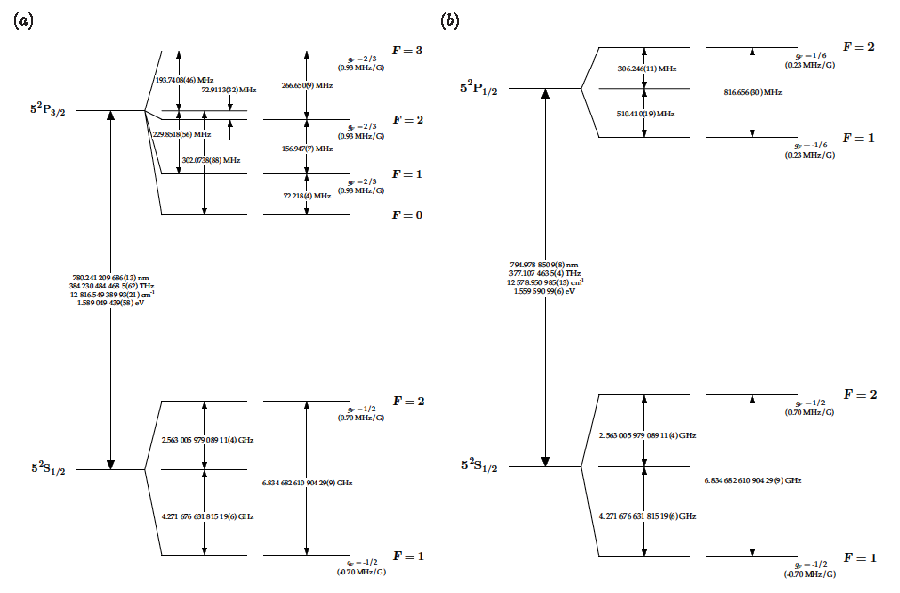
\includegraphics[width=\textwidth]{Chapter2_secs/D1andD2.pdf}
    \caption{Energy splitting of the $^{87} {\rm Rb}$ ground state and the first excited state. }
    \label{fig:D1andD2}
\end{figure}
\subsection{Zeeman splitting of $^{87} {\rm Rb}$ hyperfine ground states}\label{zeeman chpt}
The angular momentum of $^{87} {\rm Rb}$ interacts with the external magnetic field and the hyperfine states split into sub-states. Here we use perturbation theory to calculate the energy of each sub-states of $^{87} {\rm Rb}$ ground state.

For the $^{87} {\rm Rb}$ ground state, $J=1/2$ and $I=3/2$. It has hyperfine states $\ket{F=1}$ and $\ket{F=2}$. The Hamiltonian with external magnetic field is 
\begin{equation}
    \hat{H} = \hat{H}_{hfs} + (\mu_B g_J\Vec{J} + \mu_N g_I\Vec{I})\Vec{B}.
\end{equation}
Here $\mu_B = 9.27\times 10^{-24} {\rm J}\cdot {\rm T}^{-1}$ is Bohr magneton, the natural unit for expressing the magnetic moment of an electron caused by either its orbital or spin angular momentum. $\mu_N = 5.05\times 10^{-27} {\rm J}\cdot {\rm T}^{-1}$ is the nuclear magneton. $g_J$ and $g_I$ are land\'e g-factors. For $^{87} {\rm Rb}$ ground state, $g_J \approx 2.00233$ and $g_I \approx -0.00099$. 

Define the direction of magnetic field z, the Hamiltonian can be represented by the z-component of angular momentum
\begin{equation}
    \hat{H} = \hat{H}_{hfs} + \mu_B(g_J m_J + g_Im_I)B,
\end{equation}
where $m_J$ and $m_I$ are magnetic quantum numbers. $\hat{H}_{hfs}$ is diagonal in the basis of $\{\ket{F,m_F}\}$, and we can proceed by representing states $\ket{J=1/2,m_J,I=3/2,m_I}$ with $\{\ket{F,m_F}\}$ and calculate the energy of states $\ket{F,m_F}$ to second order.

\begin{align}
    &\ket{\frac{1}{2},\frac{3}{2}} = \ket{2,2}, &&\ket{\frac{1}{2},\frac{1}{2}} = \frac{\sqrt{3}}{2}\ket{2,1} - \frac{1}{2}\ket{1,1}\\\nonumber
    &\ket{\frac{-1}{2},\frac{3}{2}} = \frac{1}{2}\ket{2,1} + \frac{\sqrt{3}}{2}\ket{1,1}, &&\ket{\frac{-1}{2},\frac{1}{2}} = \frac{1}{\sqrt{2}}\ket{2,0} + \frac{1}{\sqrt{2}}\ket{1,0}\\ \nonumber
    &\ket{\frac{1}{2},\frac{-1}{2}} = \frac{1}{\sqrt{2}}\ket{2,0} - \frac{1}{\sqrt{2}}\ket{1,0}, &&\ket{\frac{1}{2},\frac{-3}{2}} = \frac{1}{2}\ket{2,-1} - \frac{\sqrt{3}}{2}\ket{1,-1}\\ \nonumber
    &\ket{\frac{-1}{2},\frac{-1}{2}} = \frac{\sqrt{3}}{2}\ket{2,-1} - \frac{1}{2}\ket{1,-1}, &&\ket{\frac{-1}{2},\frac{-3}{2}} = \ket{2,-2}\\ \nonumber
\end{align}

In the $\{\ket{F,m_F}\}$ basis,
\begin{equation}
    \hat{H}_{hfs}\ket{F,m_F} = E_{F}\ket{F,m_F}.
\end{equation}
Treat the interaction with the external magnetic field as a perturbation, the first-order perturbed energy for state $\ket{F,m_F}$ is
\begin{equation}
    \Delta E_1 = \matrixel{F,m_F}{(g_J\Vec{J}_z + g_I\Vec{I}_z)}{F,m_F}\mu_B B,
\end{equation}
and the second order perturbed energy is
\begin{equation}
    \Delta E_2 = \sum_{F',m_F'} \frac{|\matrixel{F,m_F}{(g_J\Vec{J}_z + g_I\Vec{I}_z)}{F',m_F'}|^2}{E_F-E_{F'}}(\mu_B B)^2.
\end{equation}

The energy of $\ket{F,m_F}$ states are listed here, in the units of ${\rm MHz}$, ${\rm MHz/G}$ and ${\rm MHz/G^2}$. The numbers are useful for quick estimation of the magnetic field in the lab.
\begin{align}
    \ket{2,2} &= 2.75\times 10^3h ~{\rm MHz} + 1.405h~{\rm MHz/G}\times B + 0h ~{\rm MHz/G^2}\times B^2\\\nonumber
    \ket{2,1} &= 2.75\times 10^3h ~{\rm MHz} + 0.7026h~{\rm MHz/G}\times B + 2.879\times 10^{-4}h ~{\rm MHz/G^2}\times B^2\\\nonumber
    \ket{2,0} &= 2.75\times 10^3h ~{\rm MHz} + 0h~{\rm MHz/G}\times B + 3.839\times 10^{-4}h ~{\rm MHz/G^2}\times B^2\\\nonumber
    \ket{2,-1} &= 2.75\times 10^3h ~{\rm MHz} - 0.7026h~{\rm MHz/G}\times B + 2.879\times 10^{-4}h ~{\rm MHz/G^2}\times B^2\\\nonumber
    \ket{2,-2} &= 2.75\times 10^3h ~{\rm MHz} - 1.405h~{\rm MHz/G}\times B + 0h ~{\rm MHz/G^2}\times B^2\\\nonumber
    \ket{1,1} &= -4.2896\times 10^3h ~{\rm MHz} - 0.7052h~{\rm MHz/G}\times B - 2.879\times 10^{-4}h ~{\rm MHz/G^2}\times B^2\\\nonumber
    \ket{1,0} &= -4.2896\times 10^3h ~{\rm MHz} + 0h~{\rm MHz/G}\times B - 2.879\times 10^{-4}h ~{\rm MHz/G^2}\times B^2\\\nonumber
    \ket{1,-1} &= -4.2896\times 10^3h ~{\rm MHz} + 0.7052h~{\rm MHz/G}\times B - 2.879\times 10^{-4}h ~{\rm MHz/G^2}\times B^2\\\nonumber
\end{align}

The second-order perturbation leads to the quadratic Zeeman shift which has a sizable effect when the magnetic field on the order of $ 10{\rm G}$. In some our experiments, the quadratic Zeeman shift makes the energy difference between $\ket{1,0}$ and $\ket{1,-1}$ large enough than the difference between $\ket{1,0}$ and $\ket{1,1}$. So we can effectively treat the $F=1$ manifold as a two-level system by decoupling $\ket{1,-1}$. 

For larger magnetic field, larger than $10^3{\rm G}$, the perturbation theory breaks down and {\bf Breit-Rabi formula} \cite{breit1931measurement} is useful in the case $J=1/2$. 
\begin{align}
     &E_{F=I\pm1/2} = -\frac{A_{hfs}}{4} + m_Fg_I\mu_NB \pm A_{hfs}\sqrt{1 + m_Fx x^2}, m_F \neq 2, -2\\ \nonumber
     &E_{F=2,m_F=\pm2} = -\frac{A_{hfs}}{4} + m_Fg_I\mu_NB + A_{hfs}(1 \pm x) \\\nonumber
     &x = \frac{(g_J\mu_B - g_I\mu_N)B}{2A_{hfs}}\\\nonumber
\end{align}
The energy of states $\ket{F,m_F}$ is shown in Fig.~(\ref{fig:BField}) for the magnetic field up to 15000 {\rm G}.

\begin{figure}[htbp]
    \centering
    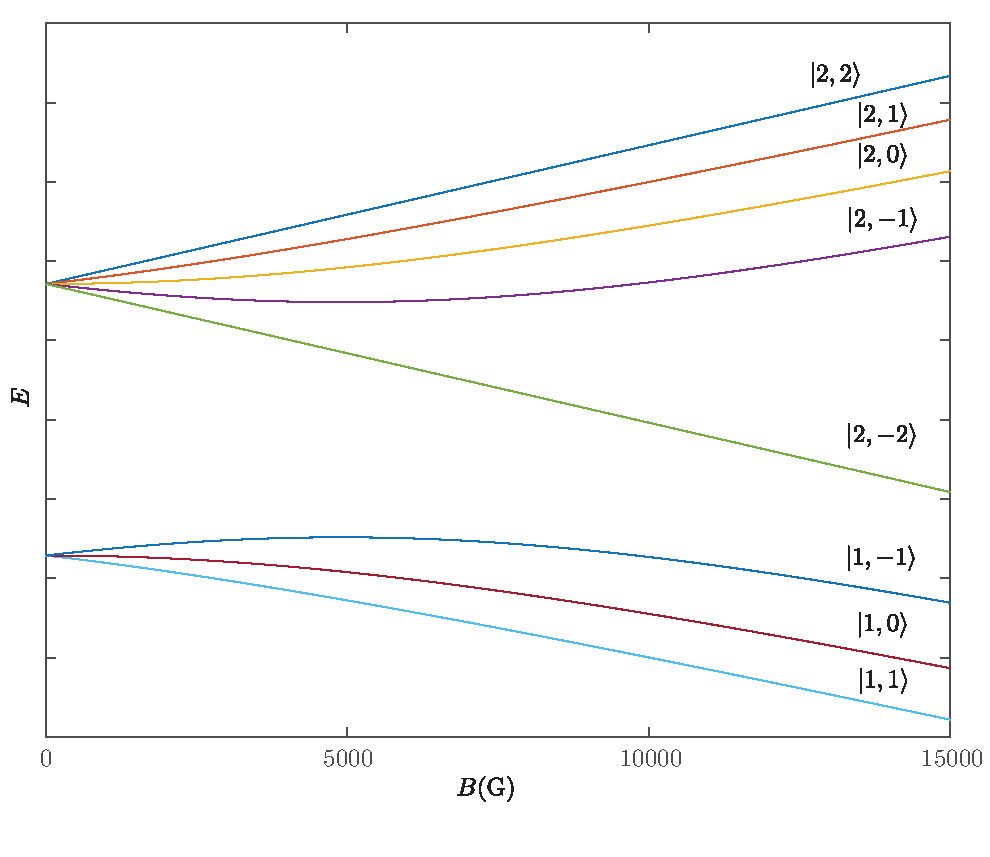
\includegraphics[width=\textwidth]{Chapter2_secs/B_field.pdf}
    \caption{Zeeman splitting of $^{87} {\rm Rb}$ ground states $\ket{F,m_F}$. }
    \label{fig:BField}
\end{figure}

\section{Laser cooling techniques}

\subsection{Two level system interacting with reservoir}

\begin{figure}[htbp]
    \centering
    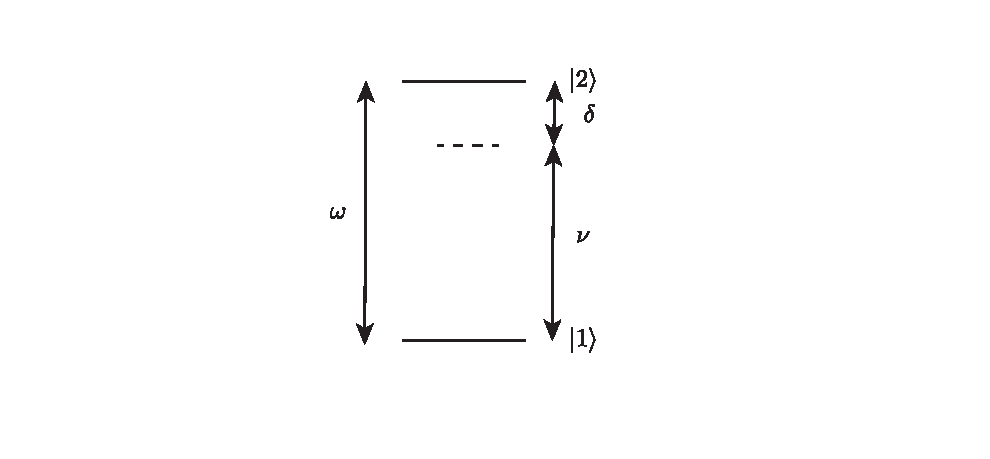
\includegraphics[width=\textwidth]{Chapter2_secs/twolevel.pdf}
    \caption{A two level system with energy difference $\omega$ in a light field with frequency $\nu$. $\delta = \nu - \omega$ is the detuning. }
    \label{fig:twolevel}
\end{figure}
A two level system shown in Fig.~(\ref{fig:twolevel}) interacts with light field via electric dipole interaction. 
\begin{equation}
    \hat{H} = -\Vec{d}\cdot \Vec{E}
\end{equation}
is the electric dipole interaction Hamiltonian where $\Vec{d} = e\Vec{r}$ is the dipole operator. The matrix element of dipole operator $\matrixel{L',m_L'}{\Vec{d}}{L,m_L}$ is nonzero only when $\Delta L = \pm 1$ and $\Delta m_L = 0$. The dipole operator doesn't interact with spin and nuclear angular momentum, so in the total angular momentum basis, the selection rule is 
\begin{equation}
    \Delta F = \pm 1.
\end{equation}
The Electric field
\begin{equation}
    \Vec{E} = E_x {\bf e_x} + E_y {\bf e_y} + E_z {\bf e_z}
\end{equation}
can be expressed in the basis of $\{ {\bf e_{\pm}},{\bf e_z}\}$,
\begin{equation}
    \Vec{E} = E_+ {\bf e_+} + E_- {\bf e_-} + E_z {\bf e_z}.
\end{equation}
Here,
\begin{equation}
    {\bf e_{\pm}} = \frac{{\bf e_x} \pm i{\bf e_y}}{\sqrt{2}}.
\end{equation}
The dipole interaction Hamiltonian is separated into the radial part and the angular part in the new basis,
\begin{equation}
    {\bf e_q}\cdot \Vec{r} = \sqrt{\frac{4\pi}{3}}\rho Y_{1,q}(\theta,\phi),
\end{equation}
here q = 1 for ${\bf e_+}$, q = -1 for ${\bf e_-}$ and q = 0 for ${\bf e_z}$, $Y_{1,q}(\theta,\phi)$ is the spherical harmonic function.

A two level system with energy difference $\omega$ interacts with electromagnetic field
\begin{equation}
    \Vec{E}(\Vec{r},t) = \Vec{E}_0 e^{-i(\nu t-\Vec{k}\cdot\Vec{r})} + \Vec{E}_0^*e^{i(\nu t-\Vec{k}\cdot\Vec{r})},
\end{equation}
the Hamiltonian is
\begin{equation}
    \hat{H} = \hbar \omega \dyad{2}{2} - (\Vec{\mu} \dyad{1}{2} + \Vec{\mu}^*\dyad{2}{1})\cdot\Vec{E}(\Vec{r},t).
\end{equation}
By transforming into a rotating frame, 
\begin{equation}
    \ket{\Tilde{2}} = e^{i\nu t}\ket{2},
\end{equation}
and neglecting the fast oscillating term $e^{\pm i\nu t}$, the Hamiltonian is transformed to
\begin{equation}
    \hat{H} = \hbar\delta \dyad{\Tilde{2}}{\Tilde{2}} + \hbar(\Omega \dyad{1}{\Tilde{2}} + \Omega^* \dyad{\Tilde{2}}{1}),
\end{equation}
Here,
\begin{equation}
    \Omega = \frac{\Vec{E}_0 \cdot \Vec{\mu}}{\hbar}.
\end{equation}
The frame transformation and the removal of the oscillating term is named after rotating wave approximation (RWA), it is widely used in atomic physics when atoms interact with near resonance high frequency optical field, and satisfying the condition $\delta \ll \nu, \omega$.

The Hamiltonian above describes a closed system, where the two level atom only interacts with the one single optical mode and the evolution of atomic states and photon states is coherent. In reality, the atom interacts not only with the optical field but also the vacuum modes in the environment. The vacuum modes are contiguous in free space and discrete in a cavity, the coupling between the atomic states to the vacuum modes leads to spontaneous emission of the excited state and causes incoherence. Wigner-Weisskopf theory \cite{scully1999quantum} represents the vacuum modes with quantized field operators and calculates spontaneous emission with Fermi's golden rule. The Hamiltonian of atomic system and vacuum modes is
\begin{equation}
    \hat{H} = \hbar \omega \dyad{2}{2} + \sum_j\hbar \nu (\hat{a}^\dag_j\hat{a}_j + \frac{1}{2}) - \sum_j(\hbar g_j \dyad{2}{1}\hat{a}_j + \hbar g_j^* \dyad{1}{2}\hat{a}^\dag_j),
\end{equation}
and $g_j$ is the coupling strength between the states $\ket{2,0}$ and $\ket{1,1_k}$. $\ket{1,1_k}$ is the state with one photon occupying mode $k$.
\begin{equation}
    \gamma = 2\pi \sum_j |g_j|^2\delta(\nu_j - \omega)
\end{equation}
is the result of spontaneous emission rate $\gamma$ and in free space
\begin{equation}
    \gamma = \frac{\omega^3|\mu|^2}{3\pi\epsilon_0\hbar c^3},
\end{equation}
which is also known as the Einstein A coefficient.

One way to describe both coherent and incoherent evolution is using density operator. The density operator is defined as
\begin{equation}
    \hat{\rho} = \sum_\alpha p_\alpha \dyad{\phi_\alpha}{\phi_\alpha}.
\end{equation}
Here, $\ket{\phi_\alpha}$ a quantum state and $p_\alpha$ is the probability that the state is in $\ket{\phi_\alpha}$. The states $\ket{\phi_\alpha}$ are not necessarily orthogonal to each other, but for the density operator representation to be valid, it has to satisfy the following condition,
\begin{equation}
    {\rm Tr}[\hat{\rho}] = 1.
\end{equation}
For any orthonormal basis $\{ \ket{n}\}$, 
\begin{equation}
    \sum_n \matrixel{n}{\hat{\rho}}{n} = 1,  and ~ {\rm Tr}[\hat{\rho}] = \sum_n \matrixel{n}{\hat{\rho}}{n},
\end{equation}
for the conservation of probability.

In the density operator representation, the expectation value of a dynamic variable $\hat{A}$ can be calculated using
\begin{equation}
    \expval{\hat{A}} = {\rm \hat{\rho}\hat{A}}.
\end{equation}

In the orthonormal basis $\{ \ket{n}\}$, the matrix element of the density operator is
\begin{equation}
    \rho_{n,n'} = \matrixel{n}{\hat{\rho}}{n'}.
\end{equation}
The diagonal elements $\rho_{n,n}$ represents the the probability that the state is in $\ket{n}$ and the off-diagonal elements $\rho_{n,n'}$ represents the expectation value of coherence between states $\ket{n}$ and $\ket{n'}$. If there exists a state $\ket{\phi}$ such that
\begin{equation}
    \hat{\rho} = \dyad{\phi}{\phi},
\end{equation}
the state represented by $\hat{\rho}$ is a pure state, otherwise, it is a mixed state. In quantum mechanics, the probability amplitude of states bear the full information, probability and coherence. The density operation representation loses the information of coherence of some states but the expectation value of coherence is preserved. 

For an open system, the physical system we are interested in interacts with the environment, or sometimes called reservoir. The reservoir can contain a large number of degrees of freedom, for example, vacuum modes and other electromagnetic fields modes. The large number of degrees of freedom of the reservoir makes it hard to study its dynamics, however, in many cases, we are not actually interested in learning about the evolution of the reservoir. In these cases, it is useful to ignore the dynamics of the reservoir and only keep the effect the reservoir has on the system. By making this assumption, the coherent evolution of the system and the reservoir is lost and there exists decoherence in the dynamic of the system, so density operator is widely used to describe the open system.

The full Hamiltonian is
\begin{equation}
    \hat{H} = \hat{H}_S +\hat{H}_R + \hat{H}_{SR} 
\end{equation}
and under Heisenberg's equation, the evolution of the density operator is
\begin{equation}
    \frac{d}{dt}\hat{\rho} = \frac{1}{i\hbar}\left[ \hat{H},\hat{\rho} \right]
\end{equation}
Assume the interaction operator takes the form
\begin{equation}
    \hat{H}_{SR}  = \hat{S}\hat{R}^\dag + \hat{S}^\dag\hat{R}.
\end{equation}
To ignore the dynamics of the reservoir and only keep the effects it has on the system, we need to make two assumptions. First, factorize the reservoir operator
\begin{equation}
    \hat{R} \approx f(t)\hat{\Tilde{R}}.
\end{equation}
The function $f(t)$ characterizes the time evolution of the reservoir, and it is often assumed that the reservoir is stationary in the stochastic process language. The auto-correlation function of $f(t)$ is defined as
\begin{equation}
    ACF_f(t-t') = \expval{(f(t)-\expval{f(t)})(f(t')-\expval{f(t')})}.
\end{equation}
The correlation time $t_c$ of the function $f(t)$ is defined as the width of the peak of $ACF_f(t-t')$. 
The first assumption of reservoir is that $t_c \ll 1$, which means the reservoir has Markovian property, it quickly forgets about its previous state does not keep the memory of interacting with the system.

The second assumption is the reservoir is large enough that the system can hardly affect its state. Again, this means that the reservoir is stationary. Under these assumptions, the dynamics of the system is derived and expressed in terms of the reduced density operator
\begin{equation}
    \hat{\rho}_S = {\rm Tr}_{\rm R} [\hat{\rho}],
\end{equation}
which takes the average of the reservoir state by tracing out the reservoir degrees of freedom.

For a two level system
\begin{equation}
    \hat{H}_S = \hbar\delta \dyad{2}{2} + \hbar(\Omega \dyad{1}{2} + \Omega^* \dyad{2}{1}),
\end{equation}
the density operator evolves under eqaution
\begin{align}\label{OBE}
    &\dot{\rho}_{22} = -\gamma(\overline{n} + 1)\rho_{22} + \gamma\overline{n}\rho_{11} + i\Omega^*\rho_{21} - i\Omega\rho_{12}\\\nonumber
    &\dot{\rho}_{11} = \gamma(\overline{n} + 1)\rho_{22} - \gamma\overline{n}\rho_{11} - i\Omega^*\rho_{21} + i\Omega\rho_{12}\\\nonumber
    &\dot{\rho}_{12} = -\frac{\gamma}{2}(2\overline{n} + 1)\rho_{12} - i\delta\rho_{12} - i\Omega^*(\rho_{22}-\rho_{11})\\\nonumber
    &\dot{\rho}_{21} = -\frac{\gamma}{2}(2\overline{n} + 1)\rho_{21} + i\delta\rho_{21} + i\Omega(\rho_{22}-\rho_{11})\\\nonumber
\end{align}
This is known as the {\bf Optical Bloch equations}, and also called \textbf{Master equation} \cite{metcalf2007laser}. The first two equations describe the evolution of the probability of occupying the states $\ket{2}$ and $\ket{1}$.  The third and fourth equations describe the evolution of expected coherence between states $\ket{1}$ and $\ket{2}$. The term $\gamma(\overline{n} + 1)\rho_{22}$ combines spontaneous emission ($\gamma\rho_{22}$) and stimulated emission ($\gamma\overline{n}\rho_{22}$). 


\subsection{Optical force}
An atomic system interacts with optical fields, which leads to stimulated emission and Rabi oscillation when the frequency of the field is near resonance. When the field is far-detuned, the atoms see a spin-independent spatial potential, the force of which drives the atoms' center-of-mass motion. Also, the atoms interact with the vacuum modes that lead to spontaneous emission. The emitted photons have nonzero momentum, so the atoms acquire the recoil momentum when the spontaneous emission happens. From the classical physics point of view, the atoms should experience a "force" in the optical fields and the definition of the "force" can be borrowed from classical physics.
\begin{equation}
    \hat{F} = \frac{d}{dt}\hat{p} = \frac{1}{ih}[\hat{p},\hat{H}]
\end{equation}
The same as classical physics, the force operator is defined as the rate of momentum change and it can be calculated for a two-level atomic system with Hamiltonian
\begin{equation}
    \hat{H} = \hbar\delta \dyad{2}{2} + \hbar(\Omega(\Vec{r}) \dyad{1}{2} + \Omega^*(\Vec{r}) \dyad{2}{1}).
\end{equation}
$\Omega(\Vec{r})$ is a function of $\Vec{r}$ for the inhomogeneous field amplitude. 
\begin{equation}
    \Vec{F} = -[\nabla,\Vec{H}(\Vec{r})] = \hbar\nabla\Omega(\Vec{r})\dyad{2}{1} + \hbar\nabla\Omega^*(\Vec{r})\dyad{1}{2}
\end{equation}
The state of the system is represented by density operator $\hat{\rho}$ and the expectation value of operator $\hat{F}$ is
\begin{align}
    \expval{\hat{F}} &= {\rm Tr}[\hat{\rho}\hat{F}]\\ \nonumber
    &=\hbar\nabla\Omega\rho_{12} + \hbar\nabla\Omega^*\rho_{21}\\\nonumber
    &=2\hbar|\Omega|^2\nabla\phi{\rm Im}\left( \frac{\rho_{21}}{\Omega}\right) + \hbar\nabla|\Omega|^2{\rm Re}\left( \frac{\rho_{21}}{\Omega}\right)\\\nonumber
\end{align}
Here, $\phi$ is the phase of the field,
\begin{equation}
    \Omega = |\Omega|e^{i\phi}.
\end{equation}
The first term is interpreted as the dissipative force and the second term the reactive force. This can be more intuitively understood when we look at the form of the force in two extreme cases.

For the steady solution of the optical Bloch equation,
\begin{align}
    &\rho_{21} = \frac{i\Omega(\rho_{22}-\rho_{11})}{\gamma_{21} - i\delta}\\\nonumber
    &\rho_{22} = \frac{R}{\gamma(\overline{n} + 1) + 2R}\\\nonumber
    &R = \frac{2\gamma_{21}|\Omega|^2}{\gamma_{21}^2 + \delta^2}\\\nonumber
\end{align}
here, $\gamma_{21}$ is the decay rate of coherence and $R$ is the optical pumping rate, the rate the atoms are pumped from the ground state to the excited state. When the field is weak,
\begin{equation}
    |\Omega| \ll \gamma
\end{equation}
the time atoms spend in the excited state is close to zero, $\rho_{22} \approx 0$. The coherence $\rho_{21}$ can be approximated with
\begin{equation}
    \rho_{21} = \Omega\frac{\delta - i\gamma_{21}}{\gamma_{21}^2 + \delta^2}
\end{equation}
The dissipative force takes the form
\begin{align}
    F_{dis} &= 2\hbar|\Omega|^2 \Vec{k}\frac{\gamma_{21}}{\gamma_{21}^2 + \delta^2}\\\nonumber
    &= \hbar\Vec{k}R\\
\end{align}
Intuitively, it means every time the atom is pumped from the ground state to the excited state, it acquires momentum $\hbar\Vec{k}$. When spontaneous emission happens, the photon is emitted in any direction with equal probability, on the average, the atom does not acquire momentum in spontaneous emission. 

In the other case, when $\delta$ is large, 
\begin{equation}
    \delta \gg |\Omega|, \delta \gg \gamma_{21}    
\end{equation}
Optical pumping rate $R \approx 0$ and the population in the excited state $\rho_{22} \approx 0$. 
\begin{equation}
    {\rm Im}\left[\frac{\rho_{21}}{\Omega}\right] \approx \frac{1}{\delta}
\end{equation}
and the reactive force takes the form
\begin{equation}
    F_{react} = \frac{\hbar\nabla|\Omega|^2}{\delta}.
\end{equation}
Effectively, the atoms see a potential
\begin{equation}
    V(\Vec{r}) = -\frac{\hbar|\Omega(\Vec{r})|^2}{\delta}
\end{equation}
The potential is spin-independent, its strength is proportional to the intensity of the field $|\Omega\Vec{r}|^2$ and the sign of $\delta$ determines if the potential is repulsive or attractive. When $\delta > 0$, the field is red detuned, and the potential is lower for stronger intensity, so the potential is attractive. When the field is blue detuned, it is repulsive.  

This potential is known as the dipole potential, it originates from the AC stark shift. Due to the large detuning, it does not drive the transition of internal states but changes the energy of the ground state so it is effectively a spin-independent potential. Dipole potential is widely used in atomic physics experiments. It can be used as an attractive trap, called a dipole trap, to trap atoms, to do evaporative cooling, and to make an optical lattice. 
The repulsive potential is also very useful, it can be used to make a 1D trap when the laser is in Laguerre-Gaussian mode \cite{salces2018equations} and make random repulsive potential (optical speckle) which is discussed in detail in Ch.~(\ref{speckle_chapter}).

    


%Chapter 3

\renewcommand{\thechapter}{3}

\chapter{Spin-Orbit coupling and Anderson localization in a cold-atom system}
In contrast to a condensed-matter system where we have little control over the material structure and the internal environment of particles, in a cold-atoms system, the external potential, the coupling between internal states and the interaction between particles can all be artificially engineered in the lab. Using the interaction between atoms and the electromagnetic field, the Hamiltonian of the atoms can be engineered to simulate that of particles in a condensed-matter system. The parameters in the Hamiltonian can be tuned by changing the intensity of the light, frequency of the light, the strength of the electromagnetic field, and etc. The high level of control over a cold-atoms system and the ability to simulate the Hamiltonian of a condensed-matter system make it an ideal platform to study fundamental condensed-matter physics that is otherwise hard to study. 

Spin-orbit coupling and Anderson localization have been realized and studied in cold atoms over the last decade. In this chapter, we briefly review the progress of spin-orbit coupling and Anderson localization in cold atoms on which our research of spin-orbit coupling enhanced transport in a random field is based.

\section{Spin-orbit coupling}



\subsection{Origin of SOC in a solid-state system}
a
\newpage
\section{Anderson Localization}

Anderson Localization (AL), introduced in 1958~\cite{anderson1958absence}, describes the localization of quantum waves in disordered media. Anderson studied the evolution of a wave packet undergoing multiple scattering processes from a random potential and proved the scattered waves can constructively interfere, leading to localization. This general starting point makes AL applicable to many quantum systems including: optical waves in disordered media~\cite{wiersma1997localization,scheffold1999localization,storzer2006observation}, electrons imperfect in crystals~\cite{anderson1958absence} and matter waves in disordered optical potentials~\cite{sanchez2007anderson,billy2008direct,roati2008anderson,kondov2011three}.

After AL was observed in multiple systems, in recent years, the research topic of AL phase transition in many body systems (may body localization) has attracted more attentions \cite{pal2010many,bardarson2012unbounded,schreiber2015observation,nandkishore2015many,choi2016exploring}. When disorder strength is above a critical value, the many body system undergoes a phase transition from thermalizing ergodic phase to a nonergodic phase. And in the nonergodic phase, the initial ordering of the many body system persists, which leads to potential application in quantum information \cite{schreiber2015observation,nandkishore2015many}. 

In this section, we first introduce a simple model from \cite{anderson1958absence} that catches the basic idea of single particle AL. Next, we review the progress of AL in cold atoms.
\subsection{Introduction to Anderson Localization}
% \begin{figure}[htbp]
%     \centering
%     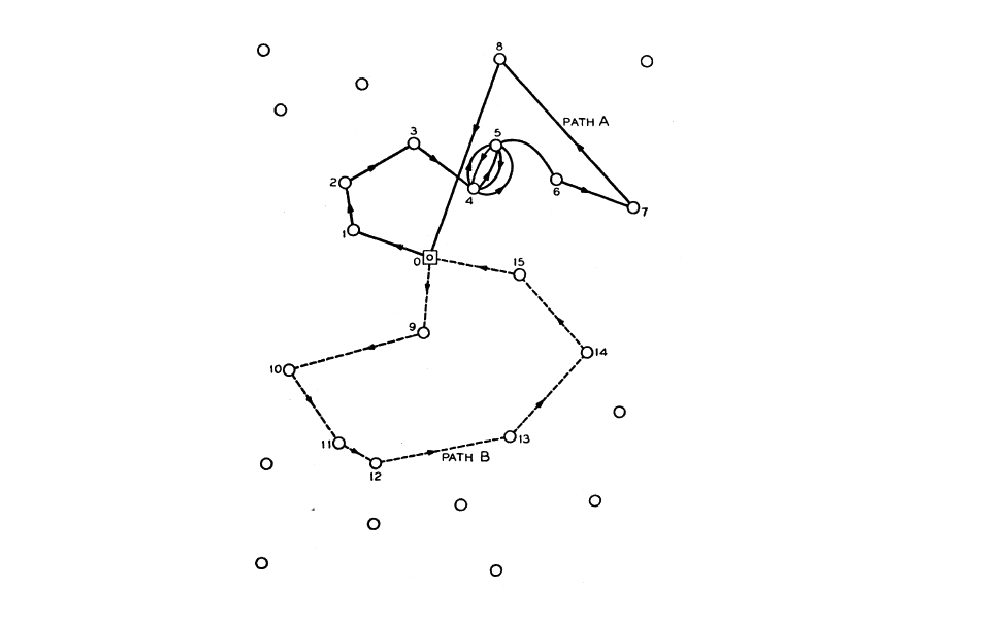
\includegraphics[width=\textwidth]{Chapter3_secs/AL1.pdf}
%     \caption{Fig.~(1) in \cite{anderson1958absence}, two kinds of scattering paths originated from lattice site 0. Path A may be large and must be summed over. Path B is a legitimate term. The potential energy at each lattice site j, $E_j$ is a random variable.}
%     \label{fig:AL1}
% \end{figure}

In the paper that introduced AL \cite{anderson1958absence}, the author studied the motion of some mobile entities in certain random lattices. It can be spins in a random field or electrons in a disordered crystal. The entities move by jumping from site to site. Starting from the most general case, the wave function of an entity can be expanded in the basis of the Wannier functions on each lattice site, 
\begin{equation}
    \hat{\psi}(\Vec{r}) = \sum_j W(\Vec{r}-\Vec{r}_j)\hat{a}_j.
\end{equation}
The Hamiltonian is
\begin{equation}
    \hat{H} = \sum_j E_j \hat{a}_j^\dag\hat{a}_j + \sum_{j<k}(V_{jk}\hat{a}_j^\dag\hat{a}_k + c.c)
\end{equation}
Here $E_j$ is the potential energy at site $j$, it is a random variable and has probability density distribution $E_j \sim \mathbb{P}(E)dE$ which is characterized by a width $W$. $V_{jk}$ is the coupling of states on site $j$ and site $k$, it can be random or non-random.

Under the following two conditions, it was proved in \cite{anderson1958absence} the wave function will be localized in a small region without diffusion. Here localization means at $t=0$, starting at site $j$, $a_j(0) = 1$, and $a_j(\infty)$ remains finite.
\begin{itemize}
    \item Low density of sites. The average coupling strength between states at different lattice sites $\langle V_{jk} \rangle < V_c$, $V_c$ is of the magnitude of $W$.
    \item $V(r)$ falls off faster than $\frac{1}{r^3}$ as $r \to \infty$.
\end{itemize}

Intuitively, the probability of diffusion from the initial site $j$ depends on the number of energy matching sites $k$ and the coupling strength between site $j$ and sites $k$. Starting from the original state at site $j$, consider the sites $k$ within the sphere of radius $r$ originated from the site $j$. As $r$ increases, the probability of finding more energy matching sites $k$ within the sphere of radius $r$ increases as $r^3$ in a 3-dimensional space. But if the coupling strength $V(r)$ decreases even faster, as $r \to \infty$, the probability the initial state diffuses to other sites remains small. So under the two conditions above, no diffusion happens and the initial state is localized.

The following discussion in \cite{anderson1958absence} shows in theory how diffusion happens. Laplace transform $a_j(t)$, the probability amplitude at site $j$,
\begin{equation}
    f_j(s) = \int^\infty_0e^{-st}a_j(t)dt
\end{equation}
Schr\"{o}dinger's equation is
\begin{equation}
    i[sf_j(s)-a_j(0)] = E_jf_j + \sum_{k\neq j}V_{jk}f_k
\end{equation}
By evaluating 
\begin{equation}
    \lim_{s \to 0^+}sf_j(s)  = a_j(0)
\end{equation}
the condition of localization can be studied. The following two infinite series describe how $f_j(s)$ evolves.
\begin{align}
    &f_0(s) - \frac{i}{is-E_0} + \sum_k \frac{1}{is-E_0}V_{0k}\left(\frac{V_{0k}}{is-E_k} + \sum_l\frac{1}{is-E_l}V_{kl}\frac{1}{is-E_k}V_{l0} + \cdots \right)f_0(s)\\\nonumber
    &f_j(s) = \frac{1}{is-E_j}V_{j0}f_0(s) + \sum_k\frac{i}{is-E_j}V_{jk}\frac{i}{is-E_k}f_0(s) + \cdots\\\nonumber
\end{align}
The infinite series describe the high-order scattering processes, diffusion happens if the initial state goes through different scattering paths that constructively interfere at other sites.  
The term 
\begin{equation}
    V_c(s) = \sum_k \frac{V_{0k}^2}{is-E_k} + \sum_{k,l}
    \frac{V_{0k}V_{kl}V_{l0}}{(is-E_k)(is-E_l)} + \cdots
\end{equation}
describes the strength of diffusion through infinite orders of scattering. By considering only the direct connections between the initial site and the neighbors, the second-order approximation is made. 
\begin{equation}
    f_0(s) = \frac{i}{is(1+K) + (i/\tau) - (E_0 - \Delta E^{(2)})}
\end{equation}
Here, 
\begin{align}
    &1/\tau = \sum_kV_{0k}^2\delta(E_k)\\\nonumber
    &K = \sum_{E_k\neq 0}\frac{V_{0k}^2}{E_k^{(2)}}
\end{align}
and $E^{(2)}$ is the second-order energy perturbation. When $\tau$ is finite, meaning there are some energy matching sites coupled to the initial site, the amplitude $a_0(t)$ decays at $e^{-t/\tau}$, and the diffusion happens. Otherwise, when no energy matching states are coupled to the initial site, the amplitude does not decay, instead, it spreads by the ratio $1/(1+K)$. No real transport happens in this case, the initial state is localized.

\subsection{AL in cold atoms}
AL was originally introduced in a condensed matter system, for example, electrons in a disordered crystal and spins in a disordered field. But there are a number of difficulties for observing AL in a condensed matter system. The interaction between electrons is hard to change, there are no good methods to directly measure the wave function of electrons in a solid. In contrast, cold atoms is an ideal platform to study AL. The interaction bwtween atoms can be tuned negligible, the wave function of atoms can be directly measured by absorption imaging and optical dipole potential has been developed that enables optical lattices.

1D AL was first observed in cold atoms in 2008 \cite{billy2008direct,roati2008anderson}. In both the experiments, the disordered potential was realized with optical dipole potential. In \cite{billy2008direct}, optical speckle from far blue detuned light was used. The statistical properties of optical speckle was well studied in the 1970s \cite{goodman2007speckle}. In \cite{roati2008anderson}, one-dimensional optical lattice perturbed by a second, weak incommensurate lattice yields localization effect. And the dependence of localization on disordered strength was studied. Later in 2011, 3D Al was realized \cite{kondov2011three}. The researchers observed three-dimensional AL of noninteracting ultracold matter by allowing a spin-polarized atomic Fermi gas to expand into a disordered
potential. In this experiment, mobility edge was extracted. In lower dimensions, actual mobility edge does not exist but quasi-mobility edge as a function of the correlation length of disordered potential has significant effect on the spread of wave function \cite{sanchez2007anderson,billy2008direct}.

\begin{figure}[htbp]
    \centering
    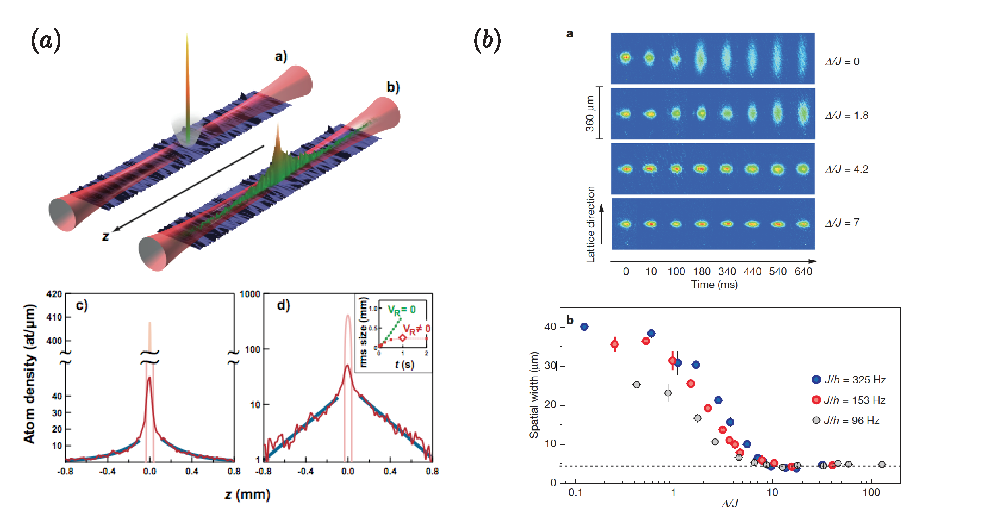
\includegraphics[width=\textwidth]{Chapter3_secs/AL2.pdf}
    \caption{First 1D AL experiments in cold atoms. (a). Fig.~(1) in \cite{billy2008direct}, Observation of exponential localization. (b). Fig.~(2) in \cite{roati2008anderson}, Probing the localization with transport. }
    \label{fig:AL2}
\end{figure}

As shown in Fig.~(\ref{fig:AL2})(a), a BEC is made in a hybrid trap consisting of a dipole trap and a magnetic trap providing longitudinal confinement. 1d optical speckle along the dipole trap was added. At t=0, the magnetic trap was turned off and the BEC started expanding due to the repulsive interaction. Without the optical speckle, the width of the atoms grow linearly in time, and as they expand, the density drops and the interaction becomes negligible. In this process, the interaction is converted into kinetic energy and determines $k_{max}$ in the momentum distribution. It is predicted in theory \cite{sanchez2007anderson} for a speckle potential with intensity correlation length $\sigma_R$, when $k_{max}\sigma_R<1$, the localized wave function has a tail that exponentially decays. This is a feature of AL. When $k_{max}\sigma_R>1$, the density profiles should have algebraic wings. $\sigma_R$ determine the quasi-mobility edge in 1D.

In Fig.~(\ref{fig:AL2})(b), 1D AL was observed in one-dimensional quasi-periodic lattice. The system is described by a Anbry-Andr\'{e} model \cite{aubry1980analyticity,harper1955single}
\begin{equation}
    \hat{H} = J\sum_m (\dyad{w_m}{w_{m+1}} + \dyad{w_m}{w_{m+1}}) + \Delta\sum_m \cos{2\pi\beta m + \phi}\dyad{w_m}{w_m}.
\end{equation}
$\ket{w_m}$ is the Wannier function at lattice m, $J$ is the tunnelling energy and $\Delta$ is the strength of disorder. The researcher make the noninteracting BEC expand along the 1D lattice, and measure the spatial density as a function of time and disorder strength. As  the disorder strength $\Delta/J$ goes above a critical value, they observed a crossover between ballistic expansion of BEC and no expansion. They demonstrated the system has the feature as in the case of purely random disorder in higher dimensions. 

These research works paved the way for more sophisticated AL studies in cold atoms and enables the interplay between AL and other well studied topics in cold atoms, for example, spin-orbit coupling.





\renewcommand{\thechapter}{4}

\chapter{Optical speckle, a Gaussian beam model}\label{speckle_chapter}
An optical speckle is a  powerful tool for creating disordered potentials for atomic systems\cite{billy2008direct,kondov2011three}.  It was studied in the 1970s \cite{goodman2007speckle}, the strength of the resultant potential is under direct experimental control: the spatial correlation length is tunable and the correlation function is well known. 

Optical speckle can be understood as the self-interfering wave field of a laser after acquiring a random phase by reflection off rough surfaces or transmission through disordered media, called a diffuser~\cite{goodman2007speckle}. We will focus on the transmission case and assume that the spatial scale of the disorder $\sigma$ is small in comparison to the laser beam size and that the diffuser transmits light uniformly. The transmitted field can be intuitively thought of as of many waves scattered from microscopic elements comprising the diffuser.  So randomness arises.  As a disordered field, optical speckle is characterized by its intensity distribution, spatial intensity correlation function, and power spectral density (PSD).  

As shown in Fig.~\ref{fig:speckle1} shows, ray optics in the paraxial limit provides a simple and useful approach to estimating the on-axis beam properties of a speckle beam a distance $z$ beyond a diffuser.  As a collimated laser beam of wavelength $\lambda$ travels through a diffuser of diameter $D_d$, it acquires a local divergence angle $\theta_d\simeq \lambda / (2 \sigma)$.   

Fig.~\ref{fig:speckle1}(a) depicts the simplest case consisting of an isolated diffuser, for which there are two qualitatively different regimes: A near-field regime with $z < D_d / (2 \theta_d)$, where the typical length scale of optical speckle is $\sigma$, and a far-field regime where the numerical aperture (NA) of the diffuser increases the speckle scale to $(\lambda / 2)\times(2 z /D_d )$.  This simple approach is insufficient because we are interested in micrometer scale speckle, which is far smaller than the 10 to 100 micrometer scale of $\sigma$ for commercial diffusers.

In Fig.~\ref{fig:speckle1}(b) we add a lens with diameter $D_L$ and focal length $f$ just after the diffuser.  In the focal plane of the lens, the speckle scale is set by the lens NA, giving a speckle length scale $\lambda f / D_L$, independent of $\sigma$. In contrast, the beam width at the focal plane $w(f) \simeq 2 f \theta_d$ is set by the speckle scale $\sigma$ and not the lens diameter.

In this chapter, we will derive the origin of these design guidelines from the paraxial wave equation.
\begin{figure}[htbp]
    \centering
    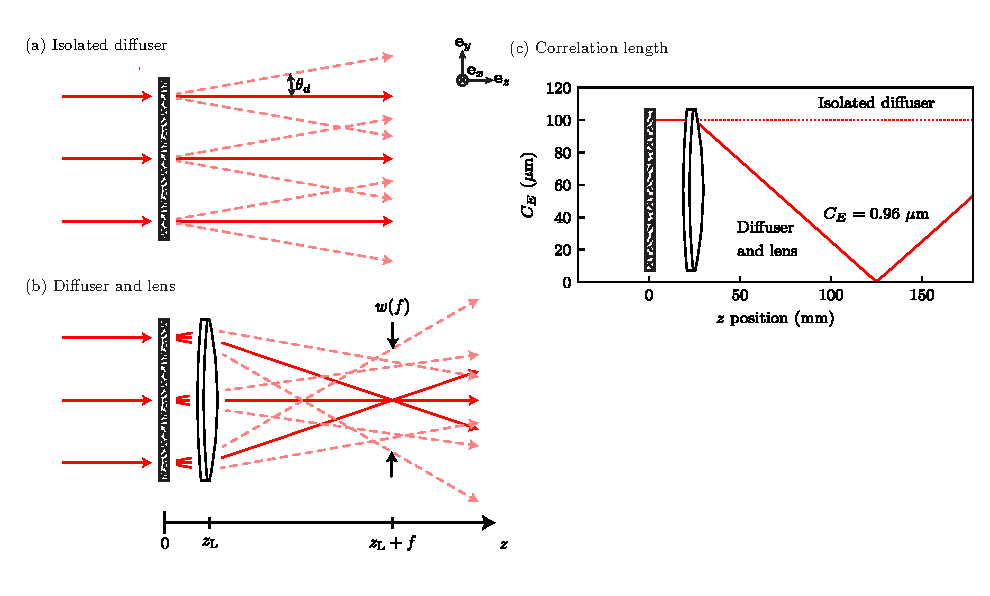
\includegraphics[width=\textwidth]{Chapter4_secs/speckle1.pdf}
    \caption{Optical speckle schematic. (a) A collimated beam is transmitted through a rough medium and its intensity is measured in plane $z$. (b) The diverged beam after the rough medium is imaged by a lens at plane $z=z_L$ and $f$ is the focal point of the lens. (c) Field-field correlation length for a Gaussian speckle beam initially with $\sigma=100\ \mu{\rm m}$ and $w=25\ {\rm mm}$ as a function of propagation distance. The red curves plot $c_E(z)$ computed with (solid) and without (dashed) a lens with focal length $f=100\ {\rm mm}$ at $z_L=25\ {\rm mm}$. }
    \label{fig:speckle1}
\end{figure}

\section{Gaussian beam equations with speckle}
We focus on monochromatic optical electric fields $E({\bf x}, t)$ with angular frequency $\omega$ traveling predominantly along ${\bf e}_z$.  Such waves can be decomposed as $E({\bf x}, t) = E_\perp({\bf r}; z) \exp[i(k_0 z -\omega t)]$, where $E_\perp({\bf r}; z)$ describes the transverse structure of the electric field with the high spatial frequencies associated with the nominal propagation along ${\bf e}_z$ factored out.  For spatial scales in excess of the optical wavelength the transverse field obeys the paraxial wave equation
\begin{equation}\label{para equation}
    -2i k_0 \partial_z E_\perp({\bf r}; z) = \left[-\nabla_\perp^2 + k_0^2 \chi({\bf r}; z)\right] E_\perp({\bf r}; z)
\end{equation}
traveling in a material with relative susceptibility $\chi({\bf r}; z)$.  We will suppress the $\perp$ subscript in the remainder of our discussion.

Upon traversing through a thin but disordered material with susceptibility $\chi({\bf r}) $ and thickness $\delta z$, an initially Gaussian wave field $E^-({\bf r}, 0) = E_0\exp{-{\bf r}^2/w^2}$ acquires a position dependent complex phase $\phi({\bf r}) = \chi({\bf r}) k_0 \delta z/2$.  The resultant field
\begin{equation}
    E^+({\bf r}, 0) = E^-({\bf r}, 0)\exp[- i \phi({\bf r})]
\end{equation}
carries the imprint of the disordered medium. The field a distance $z$ beyond the speckle plate follows from
\begin{align}\label{para field}
    E({\bf r}; z) &= \frac{-i k_0}{2\pi z}\int d^2{\bf r'} E^+({\bf r'}; 0) e^{-i k_0|{\bf r}-{\bf r'}|^2/2z},
\end{align} 
the formal solution to the paraxial wave equation Eq.~(\ref{para equation}).  We model typical diffusion plates, for which: (1) the correlation function of the susceptibility $\langle \chi({\bf r_1})\chi({\bf r_2}) \rangle$ depends only on relative distance $|{\bf r_1}-{\bf r_2}|$, where $\langle ... \rangle$ denotes the ensemble average over disorder realizations. (2) the variation of the imprinted phase $\phi({\bf r})$ is much larger than $2\pi$ with
\begin{align}\label{eq:zeromean}
\langle \exp\left[- i \phi({\bf r}_1)\right]\rangle &= 0,
\end{align} 
i.e., $\phi({\bf r})$ is uniformly distributed over the interval $[-\pi,\pi]$.
 
We turn to the field-field correlation function
\begin{equation}\label{C_E}
\begin{aligned}
    C_E({\bf r}_1,{\bf r}_2;z) &=\langle E({\bf r}_1; z)E^\ast({\bf r}_2; z)\rangle\! -\! \langle E({\bf r}_1; z)\rangle\langle E^\ast({\bf r}_2; z)\rangle
\end{aligned}
\end{equation}
to characterize the statistical properties of the disordered electric field.  Eq.~\eqref{eq:zeromean} implies that the second term is zero.  At $z=0$, the uniform phase distribution implies $\langle E^+({\bf r}; 0) \rangle = 0$, giving
\begin{align*}
\frac{C_E({\bf r}_1,{\bf r}_2;0)}{E_0^2 } &= \exp\left(-\frac{{\bf r}_1^2 + {\bf r}_2^2}{w^2}\right) \langle \exp\left\{- i \left[\phi({\bf r}_1)-\phi({\bf r}_2)\right]\right\}\rangle.
\end{align*}
Under the assumptions of the typical diffusion plates, we model the phase-phase correlation function 
\begin{align}\label{gaussian C_E}
\langle \exp\left\{- i \left[\phi({\bf r}_1)-\phi({\bf r}_2)\right]\right\}\rangle &= \exp(-\frac{|{\bf r}_1-{\bf r}_2|^2}{\sigma^2}), 
\end{align} 
with a Gaussian decay of width $\sigma$ that is amenable to the following analytic treatments.  The relation
\begin{align}\label{eq:sum_CE_zero}
\langle \exp\left\{- i \left[\phi({\bf r}_1)+\phi({\bf r}_2)\right]\right\}\rangle &= 0, 
\end{align} 
that follows from Eq.~\eqref{eq:zeromean}, in conjunction with the assumption that the correlation function depends only on relative distance, will be useful as well.

We first consider the case illustrated by Fig.~\ref{fig:speckle1}(a) where a Gaussian beam goes through a large disordered medium. The field-field correlation function at all positions following the disordered medium  can be exactly computed and takes the form 
\begin{align}
\frac{C_E({\bf r}_1,{\bf r}_2;z)}{E_0^2} =& \left[\frac{w}{w(z)}\right]^2 \exp(-ik_0\frac{{\bf r}_1^2 - {\bf r}_2^2}{2 R(z)})\label{eq:C_E}\\
&\times \exp(-\frac{{\bf r}_1^2 + {\bf r}_2^2}{w(z)^2})\exp(-\frac{|{\bf r}_1-{\bf r}_2|^2}{\sigma(z)^2}) \nonumber 
\end{align}
reminiscent of that of Gaussian beams.

This correlation function is characterized in terms of three $z$-dependent functions: the beam waist $w(z)$, the radius of curvature $R(z)$, and the correlation length $\sigma(z)$.  Each of these is simply related to a reduced Rayleigh range $z_{\rm R}^* = z_{\rm R}/M$, with conventional Rayleigh range $z_{\rm R} = k_0 w^2/2$ and beam quality factor $M^2 = 1+2w^2/\sigma^2$.  The resulting coefficients
\begin{align}
    \left[\frac{w(z)}{w}\right]^2 &= \left[\frac{\sigma(z)}{\sigma}\right]^2 = 1+\left(\frac{z-z_0}{z_{\rm R}^*}\right)^2\label{eq:rayleigh}
\end{align}
and
\begin{align}
    \frac{R(z)}{z-z_0} = 1 +\left(\frac{z_{\rm R}^*}{z-z_0}\right)^2
\end{align}
take the same form as a usual Gaussian beam focused at $z_0$.  Lastly, as in Fig.~\ref{fig:speckle1}(b), an ideal lens with focal length $f$ at position $z_L$ gives new Gaussian beam parameters defined by
\begin{align}\label{lens making}
\frac{w^\prime}{w} &= \frac{\sigma^\prime}{\sigma} = f \left[\left(z_0'-z_L-f\right)^2+z_{\rm R}^{*2}\right]^{-1/2}
\end{align}
and
\begin{align*}
\left(z_0^\prime-z_L\right)^{-1} &=  f^{-1} - \left[\left(z_L-z_0\right) + \frac{z_{\rm R}^{*2}}{z_L-z_0-f} \right]^{-1}
\end{align*}

where the first expression defines the magnification and the second is analogous to the usual lens makers equation~\cite{Self1983}.  While this leaves $M^2$ unchanged, the Rayleigh range is altered owing to the change in $w$.  All together these relations fully define field-field correlation function $C_E$ throughout an ideal imaging system. 

In most quantum-gas experiments, optical potentials are created using laser light in the far detuned limit, thereby experiencing a potential proportional to the optical intensity
\begin{equation}\label{intensity}
    I({\bf r}; z) = \frac{c \epsilon_0}{2} \left|E({\bf r}; z)\right|^2
\end{equation}
not the electric field directly.  The ensemble-averaged intensity 
\begin{align}
\langle I({\bf r}; z) \rangle &= \frac{c \epsilon_0}{2} C_E({\bf r},{\bf r}; z), \label{eq:intensity}
\end{align}
simply related to the field-field correlation function in Eq.~(\ref{eq:C_E}), contains no information about the optical speckle except for the changed $M^2$.

As discussed in the next section, the power spectral density (PSD) of the intensity
\begin{align}
    \rho({\bf k}; z) &= \langle \tilde{I}({\bf k};z)\tilde{I}^*({\bf k};z)\rangle\nonumber \\
    &=  \frac{\pi^2w^2(z)}{4M^2}\exp{-\frac{{\bf k}^2w^2(z)}{4M^2}},\label{psd}
\end{align}
computed using Eq.~\eqref{eq:C_E}, describes the momentum-change imparted by the speckle potential to a moving atomic wavepacket.
\section{Correlation length}
The field-field correlation length
\begin{align}
    c_E(z)^2 &= \frac{\iint |C_E({\bf r}_1,{\bf r}_2; z)||{\bf r}_1-{\bf r}_2|^2d^2{\bf r}_1d^2{\bf r}_2}{\iint |C_E({\bf r}_1,{\bf r}_2; z)|d^2{\bf r}_1d^2{\bf r}_2}\\
    &= \frac{2 w(z)^2 \sigma(z)^2}{2w(z)^2 + \sigma(z)^2} \approx \sigma(z)^2
\end{align}
obtained from Eq.~(\ref{eq:C_E}), sets the scale over which the electric field retains its spatial coherence.  The field-field correlation length is minimized at $z=z_0$, and is always larger than $\sigma$.  Generally, speckle beams operate in the regime $w \gg \sigma$, where there are many speckle grains within a large beam, giving the final approximate relation. 

As was already noted in our ray-optics discussion, this has important implications for experiment design.  For cold atom experiments such as ours, the large momentum-change imparted by short-length scale speckle is essential, where a correlation length at or below the micron scale is desirable.  Since the correlation length available for typical commercial diffusers ranges from $10\ {\rm \mu m}$ to $100\ {\rm \mu m}$, an additional focusing stage is required.  

A focusing lens can easily take the $10\ {\rm \mu m}$ to $100\ {\rm \mu m}$ correlation length available for typical commercial diffusers and create a beam with sub-micrometer correlation length at its focus.  Fig.~\ref{fig:speckle1}(c) compares the correlation length of a beam with (red solid) and without (red dashed) a focusing lens for the specific case of an initial laser beam of wavelength $\lambda = 532\ {\rm nm}$ with Gaussian beam parameters: focal point $z_0=0$, beam waist $w = 25\ {\rm mm}$ and correlation length $\sigma = 100\ \mu{\rm m}$.  This beam is focused by a lens of focal length $f=100\ {\rm mm}$, the correlation length at the focus is $c_E=0.96\ \mu{\rm m}$.  The remaining derived beam parameters are
$M^2 \approx 1.25\times10^5$, $z_R \approx 3.7\ {\rm km}$, and $z_R^* \approx 10.4\ {\rm m}$. 

In \cite{yura1999three}, the space–time evolution of three-dimensional (3D) optical speckle is studied using the ABCD ray-matrix techniques. The optical speckle they studied results from a diffuse object that is illuminated by a Gaussian-shaped laser beam. The field-field correlation length obtained from this approach agrees with our results. In addition, the intensity-intensity correlation length in $z$ direction is calculated in \cite{yura1999three}. In the case the optical speckle is focused by a lens with focal length $f$, the on-axis intensity-intensity correlation length in $z$ direction $L_z$ is of the order of the depth of focus $4f^2/kw^2$. Using the parameters in Fig.~\ref{fig:speckle1}(c), in the focal plane, $L_z \approx 5.4~{\rm \mu m}$. In the free propagation case, $L_z$ grows as $4z^2/kw^2$, and $L_z \gg c_E(z)$ in the far field where $z \gg w$.

\section{Impact of apertures}
In the case of focusing optical speckle as shown in Fig.~\ref{fig:speckle1}(b), a lens of focal length $f$ and diameter $D_L \ll w$ is placed at $z=z_L \leq k_0\sigma^2$. The field in the plane $z=z_L$ before the lens, $E^-({\bf r};z_L)$ is essentially unchanged from field $E^+({\bf r};0)$. The field $E^-({\bf r};z_L)$ passes through the lens aperture, where it acquires a position dependent phase and is truncated outside the lens. The emerging field $E^+({\bf r};z_L)$ propagates to the focal plane $z=f+z_L$ where it is 
\begin{equation}\label{field in z}
    E_f({\bf r}) = \frac{-i k_0}{2\pi f}e^{-i k_0{\bf r}^2/2f}\int \displaylimits_{|{\bf r'}|<\frac{D_L}{2}} d^2{\bf r'} E^+({\bf r'}; 0) e^{i k_0{\bf r}\cdot{\bf r'}/f}.
\end{equation}
When $\sigma \ll D_L \ll w$, the field-field correlation function at the focal plane is
\begin{align}
C_{E,f}({\bf r}_1,{\bf r}_2) \approx & C_0\exp[-\frac{ik_0({\bf r}_1^2-{\bf r}_2^2)}{2f}]\\
&\times\exp[\frac{-k_0^2\sigma^2({\bf r}_1 + {\bf r}_2)^2}{16f^2}]\frac{J_1(k_c \Delta r/2)}{k_c\Delta r /2}.\nonumber
\end{align}
Here $C_0 =  k_0^2E_0^2D_L^2\sigma^2 / 8f^2$ is the peak correlation amplitude; $\Delta r = |{\bf r}_1-{\bf r}_2|$ is the relative position coordinate; and $J_1$ is a Bessel function of the first kind.  The ratio 
\begin{align}
k_c &= k_0\frac{D_L}{f}\label{kc}
\end{align}
is a cutoff above which the PSD of the intensity
\begin{align}
    \rho_f(k) = C_0^2 \frac{2}{\pi k_c^2}\left[ \cos^{-1}\left(\frac{k}{k_c}\right)
     -\frac{k}{k_c}\sqrt{1-\frac{k^2}{k_c^2}}\right]\label{psd_image}
\end{align}
is strictly zero.  Eq.~\eqref{psd_image} is valid near the optical axis where $|{\bf r}_1|,|{\bf r}_2| \ll w(z)$.
\section{Field and intensity probability distribution}\label{prob sec}
In the previous sections, we focused on the average properties of speckle fields.  Here we extend this discussion to predict the probability distribution of electric field strength $P(E)$ and intensity $P(I)$.  Our approach focuses first on $P(E)$, and consists of two steps: (1) we find the regime when the central limit theorem applies, thereby assuring a Gaussian probability distribution; (2) we identify $\langle E \rangle$ and $\langle E^2 \rangle$ as the lowest moments of the distribution, fully defining the Gaussian distribution.

We now interpret the electric field
\begin{align*}
    E({\bf r}; z) &= \frac{-i k_0}{2\pi z}\int d^2{\bf r'} E^-({\bf r}')e^{-i \phi({\bf r'}) } e^{-k_0|{\bf r}-{\bf r'}|^2/2z},
\end{align*} 
of Eq.~\eqref{para field} as a random variable constructed from a sum over incoherent complex phasors.  The cross correlation function (CCF) $\langle E({\bf r}_1; z) E({\bf r}_2; 0)\rangle$ specifies the range over which the initial random field contributes to the final field.  The closed form expression for this CCF is similar to the field-field correlation function in Eq.~\eqref{eq:C_E}; the length scale for the decay of correlations $\sigma_{\rm CCF}(z)$ again obeys  Eq.~\eqref{eq:rayleigh}, but with $M_{\rm CCF}^2=(1 + w^2/\sigma^2 )^2$.  When $w\gg\sigma$, i.e., the initial waist is much larger than the speckle size,  the resulting Rayleigh range reduces to $z_{\rm R, CCF} = k_0 \sigma^2/2$: as if each random source was an individual Gaussian beam with extent $\sigma$.  The criterion that a field $E({\bf r}; z)$ have contributions from many incoherence sources is therefore $\sigma_{\rm CCF}(z)/\sigma\gg1$, i.e., $z\gg z_{\rm R, CCF}$.  

This identifies the central limit theorem's regime of applicability, and we now consider $E({\bf r}; z)$ as a complex valued Gaussian random variable.  The probability distribution for electric field is therefore a function of two independent degrees of freedom, here we select the quadrature variables $E$ and $E^*$, giving $P(E, E^*)$.   Most moments of this quantity are easy to identify using Eqs.~\eqref{para field}, \eqref{eq:zeromean}, \eqref{gaussian C_E} and \eqref{eq:sum_CE_zero}: $\langle E \rangle = \langle E^2 \rangle = 0$, and similarly for $E^*$.   Then Eqs.~\eqref{C_E} and the following discussion assure us that  $\langle E E^* \rangle = \langle |E|^2 \rangle$ takes on a non-zero value.  Together these fully define the Gaussian probability distribution for electric fields
\begin{align}
    P(E, E^*) &= \frac{1}{\pi \langle |E|^2 \rangle} \exp\left(-\frac{|E|^2}{\langle |E|^2 \rangle}\right)\label{eq:dist_fields},
\end{align}
and using Eq.~\eqref{eq:intensity}, the intensity distribution
\begin{align}
    P(I) &= \frac{1}{\langle I \rangle} \exp\left(-\frac{I}{\langle I \rangle}\right) \label{P of int}
\end{align}
follows directly.  The intensity of a speckle field obeys an exponential distribution and the mean of speckle intensity $\langle I \rangle$ should be equal to its standard deviation $\sqrt{\langle I^2 \rangle}$.
\section{Simulated speckle and the comparison to experiment}

\begin{figure}[tbp]
    \begin{center}
    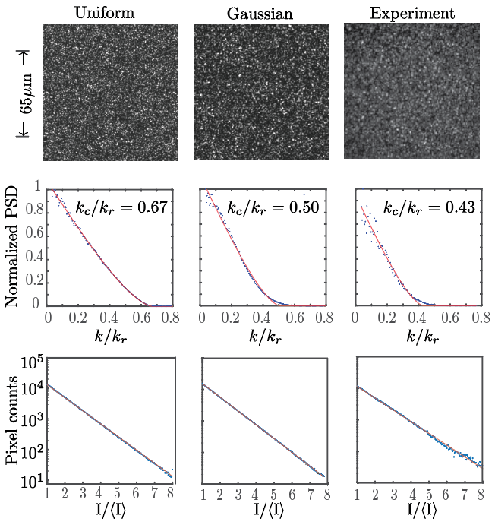
\includegraphics{Chapter4_secs/optical_speckle.pdf}
    \end{center}
    
    \caption{Simulated and measured optical speckle. The columns in the figure correspond to: simulated speckle with uniform laser beam,  simulated speckle from a Gaussian laser beam and measured speckle. In each column, the first row shows the intensity of the optical speckle field. The second row shows the PSD of the intensity shown in the first row (symbols).  The red curve shows a fit of Eq.~(\ref{psd_image}) to the data, along with the resulting $k_c$. The third row histograms the  intensity from the first row. }
    \label{fig:Optical speckle}
\end{figure}

Having now fully set the stage for understanding and creating speckle laser beams, we turn to laboratory confirmation of key prediction of these models relevant to cold atom experiment: the field-field correlation length $C_E$ and the distribution of intensities $P(I)$.

In our lab, we directed a collimated laser beam (waist $w\approx25\ {\rm mm}$) through a diffuser (divergence angle $\theta_d = 0.5^\circ$, and aperture $D=20\ {\rm mm}$) focused immediately by a lens (focal length $f = 30 {\rm mm}$) as depicted in Fig.~(\ref{fig:speckle1}) and quantified the optical speckle formed at the focal plane.  We then imaged the optical speckle onto a charge coupled device (CCD) camera with Keplerian telescope with magnification $M=46$.  The CCD's $1024 \times 1280$ array of $4.8\ \mu {\rm m}$ pixels gave a $100\ \mu{\rm m} \times 130\ \mu{\rm m}$ magnified field of view with $0.1\ \mu {\rm m}$ pixels.

Our analytic results for $C_E$ are valid in the Gaussian beam limit ( $w\ll D$) or uniform illumination limit ($w\gg D$).  Because our experiment has $w\approx D$, we numerically simulated the optical speckle to compare with our measurements and both models.

For the numerical simulation, the desired optical speckle field $E_{i,j}$ is represented by a $1024 \times 1280$ array at the focal point of the lens.  We use the optical Fourier transform property of lenses to compute this efficiently, whereby the field a focal distance beyond the lens is related to the Fourier transform of the field a focal distance prior to the lens (which we will term the Fourier plane).  An important aspect of this method is that the $0.1\ \mu {\rm m}$ grid spacing in the focal plane transforms to a $1.5\ {\rm mm}$ grid spacing in the Fourier plane.

Our simulation progresses as follows.  (1) We first initialize $E_{i,j}(z=0)$ to the field of either a uniform field or a Gaussian beam.  (2) We then imprint random phases on each point~\footnote{The grid size is much larger than the correlation length of the diffuser, so the imprinted phase at each grid point is uncorrelated with all other points.}.  (3) We set the field outside our physical aperture to zero.  (4) Then we back-propagate the field to the Fourier plane and take the Fourier transform to obtain the field at the focal plane.

Fig.~(\ref{fig:Optical speckle}) compares our measured speckle with numerics and our analytic model; the three columns depict: the case of a uniformly illuminated aperture, Gaussian illumination, and experiment.   The top row shows that intensity at the focal plane is qualitatively similar for all three cases. In the middle row, the PSD (computed from the intensity in the top row, and plotted by blue symbols), highlights the differences.  In each case, we fit Eq.~(\ref{psd_image}) the PSD and extract $k_c$ from the fits (red curves).  Because  Eq.~(\ref{psd_image}) was derived for a uniformly illuminated aperture it provides a good fit to the uniform illumination case but deviates at large $k$ for Gaussian illumination and experiment.  In contrast, the numerics for Gaussian illumination and the experiment are indistinguishable.  
% In the numerical simulation, we account for the $20{\rm mm}$ clear aperture of the lenses and diffuser. In the uniform case, our analytical model calculates $k_c = 0.62k_r$ and the numerically calculated PSD agrees with Eq.~(\ref{psd_image}) very well. 
In the bottom row, we histogram the intensity distribution and verify that in all three cases we recover the expected exponential fall-off.
\renewcommand{\thechapter}{4}

\chapter{Enhanced transport of SOC Bose gases in disordered potentials, model and simulation}

\renewcommand{\thechapter}{6}

\chapter{The evolution of BECs in disordered potentials}

In this chapter, we report the experimental study of the evolution of BECs in disordered potentials. In Sec.~(\ref{optical_design}), we present the optical design diagrams of both the speckle beam and the Raman beams which are used to generate spin-orbit coupling as discussed in Sec.~(\ref{soc}). And we discuss the reasons behind these designs. In Sec.~(\ref{speckle_pulsing}), we show the experimental results of the evolution of BECs under the pulses of speckle potentials, both in the short term and in the long term. Based on our analytical study and numerical simulations, we show the results of characterizing the PSD of the speckle potentials by using the short-term speckle pulses data and measuring the average speckle potential by using the long-term speckle pulses data. In Sec.~(\ref{transport}), we measure the deceleration of spinless BECs in the speckle potentials and compare them with our simulation results shown in Ch. (\ref{chpt 5}).
\section{Optical design}

\subsection{Speckle beam design}\label{speckle_design}

\begin{figure*}
    \centering
    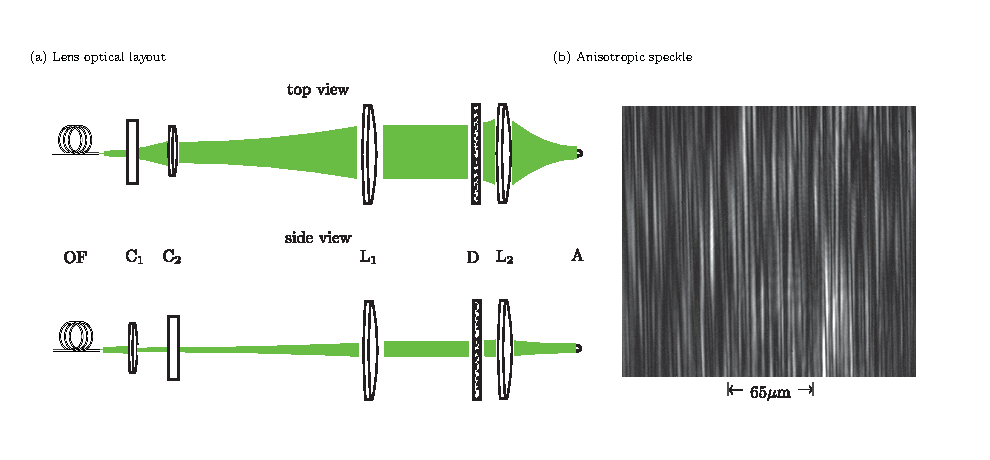
\includegraphics{Chapter6_secs/speckle_design.pdf}
    \caption{Optical design. (a). The design of optics viewed in two directions. OF denotes optical fiber. Lenses $C_1$ and $C_2$ are cylindrical lenses: $C_1$ focuses the beam in the vertical direction; and $C_2$ focuses the beam in the horizontal direction. $L_1$ is a spherical lens that collimates the beam. D is the optical diffuser that imprints random phase on the beam. $L_2$ is an aspherical lens that focuses the beam to the atoms labelled with A. (b) Experimental image of optical speckle with anisotropic correlation length.}
    \label{fig:design}
\end{figure*}

In practice, the speckle beam must satisfy two requirements.
The first is anisotropic field-field correlation length: small along $\ex$ and large along $\ey$ and $\ez$ so that high-momentum scattering occurs predominantly along $\ex$. 
The second is that the beam width along $\ex$ should uniformly illuminate the elongated atomic ensemble (with expected diameter of about $50\ \mu{\rm m}$).
To observe the effect of SOC-suppressed transport, the speckle potential must couple energy matched states across the SOC gap, shown by the dashed line in Fig.~\ref{fig:Dispersion relations}(c). 
This implies PSD of speckle potential along $\ex$ satisfies $k_c\gtrsim 4\kr$, informing the selection of beam-size and lenses.
The requirement that the correlation length along $\ey$ be large implies that at the diffuser plate, the beam be much smaller along $\ey$ than along $\ex$.

To satisfy these joint requirements, we created the speckle beam shown in Fig.~\ref{fig:design}(a), that begins with a $532{\rm nm}$ laser beam emanating from an optical fiber. 
The beam out of an optical fiber travels through the cylindrical lens $C_1$ (focusing along $\ey$) before encountering a cylindrical lens $C_2$ (focusing along $\ex$) as shown in Fig.~\ref{fig:design}(a), given more rapid divergence along $\ex$ than $\ey$.
The beam is then collimated by $L_1$, a $f = 250\ {\rm mm}$ spherical lens, giving beam width of around $25\ {\rm mm}$ along $\ex$ and less than $500\ \mu{\rm  m}$ along $\ey$ (on the same scale the diffuser plate's correlation length). 

The beam then traverses the diffuser plate (Edmund Optics part number \#47-680, with divergence angle $\theta_d = 0.5^\circ$)  and is focused by $L_2$, a $f = 30\ {\rm mm}$ lens.
Figure~\ref{fig:design}(b) shows a test image of the speckle beam at the focal plane, its intensity correlation length is less than $0.5\ {\rm \mu m}$ along $\ex$ and about $10\ \mu{\rm  m}$ along $\ey$. 
The beam widths along both directions are about $250\ \mu{\rm m}$.


\subsection{Raman beams design}
We generate Raman coupling with $\lambda \approx {\rm 790nm}$ laser. The recoil vector of the laser is 
\begin{equation}
   k_{\rm r} = \frac{2\pi}{\lambda}.
\end{equation}
When two Raman beams intersect at an angle $\theta_R$ as shown in Fig.~(\ref{fig:raman_design}), the two photon recoil vector is
\begin{equation}
    \kr = k_{\rm r}\sin{\frac{\theta_R}{2}}.
\end{equation}
As shown in Fig.~(\ref{fig:Dispersion relations}c), the detuning between states $\ket{q+\kr,\uparrow}$ and $\ket{q-\kr,\downarrow}$ is
\begin{equation}
    \Delta(q) = \frac{2\hbar^2q\kr}{m} + \delta.
\end{equation}
$\delta$ here is the detuning between two Raman beams and $\Delta(q)$ increases with $\kr$. As described in Sec.~(\ref{soc}), one step in the process we prepare the SOC quasimomentum state $\ket{q_0,-}$ is adiabatic evolution. We achieve this by ramping up the Raman coupling strength from zero to $\Or$ on a time scale slow compared to $\hbar/\Delta(q_0,0)$. In experiment, we prefer to ramp up Raman coupling fast, limited by the lifetime of BEC, but still slow compare to $\hbar/\Delta(q_0,0)$. For this reason, we want to make $\kr$ as large as possible. In this design, it means large enough intersection angle $\theta_R$. On the other hand, we also want $\kr$ to be small enough that $k_c/\kr$ is large enough the speckle potential can couple more energy matching stats shown as the circles in Fig.~(\ref{fig:Dispersion relations}). Here $k_c$ is the cut off in the PSD of the speckle potential. In our experiment, the two Raman beams and the speckle beam are focused to the atoms by the same lens $L_1$, at the largest $\theta_R$, $k_c/\kr \approx 3$. 

For the above two reasons, there is a trade off between small and large $\theta_R$, we need to find out the best angle by experimentally test. So for the optical design, we need to be flexible in changing the angle. As shown in Fig.~(\ref{fig:raman_design}), we use a triangular prism to combine the two Raman beams and align them to be parallel. The triangular prism is put on a transnational stage which can move in the perpendicular direction of the two incident Raman beams. By moving the prism, the distance between the two Raman beams can be changed and the distance is map to the distance at lens $L_1$ which determines the angle $\theta_R$.

\begin{figure*}
    \centering
    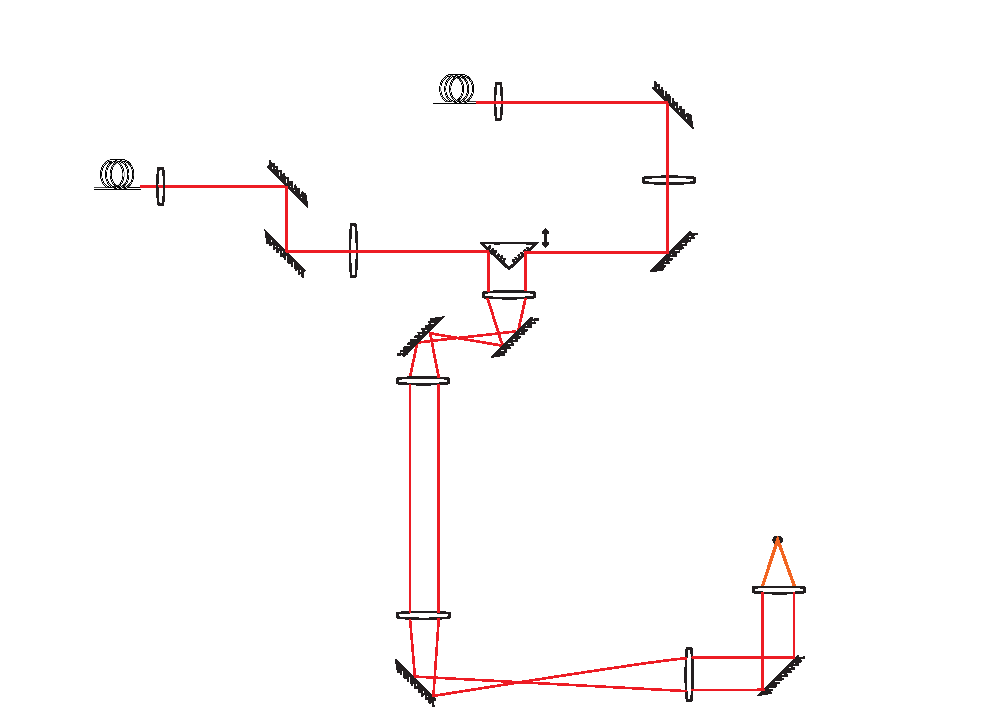
\includegraphics{Chapter6_secs/Raman_design.pdf}
    \caption{Raman beams design. The optical diagram of Raman beams. We use a triangular prism to align two Raman beams, the distance between two Raman beams at the prism is mapped to the distance at the lens $L_1$ by two relay imaging systems. The prism is put on a transnational stage which can move in the perpendicular direction of the two incident Raman beams. By moving the prism, the distance between the two Raman beams can be changed which determines the angle $\theta_R$.}
    \label{fig:raman_design}
\end{figure*}
\section{Evolution of spinless BEC under speckle pulsing}\label{speckle_pulsing}
In Ch.~(\ref{speckle_chapter}), we derived a Gaussian beam model of the speckle beam and calculated the field-field correlation function, the PSD, and the intensity distribution. In the experiments, the engineered speckle beam is focused at the atoms and it is hard to directly measure the average intensity of the speckle beam at the atoms. Direct measurements of the PSD and $k_c$ is even harder. In some experiments carried out previously that involved a speckle beam \cite{kondov2011three, billy2008direct}, the researchers set up an identical beam at the test bench and measure the average intensity and the PSD of the test speckle beam. The power and the PSD of the speckle beam in the experiments are assumed to be the same as those of the test beam, but no direct measurements were done to the best of our knowledge. Inspired by \cite{huckans2009quantum}, we designed and carried out an experiment that allowed us to measure the average intensity and the PSD of the speckle beam by using the evolution of spinless BECs under the speckle potentials.

\begin{figure*}
    \centering
    \includegraphics{Chapter6_secs/speckle_pulsing_images.pdf}
    \caption{Absorption images of atoms after the evolution under speckle potentials and TOF. The BECs are released from the dipole trap, the pulses of the speckle potentials are turned on immediately for a various amount of time, followed by TOF. The absorption images are stacked up horizontally according to the speckle pulse duration.}
    \label{fig:speckle_pulsing_imgs}
\end{figure*}

In \cite{huckans2009quantum}, the diffraction of a Bose-Einstein condensate from a one-dimensional optical lattice is studied. In very short time,
\begin{equation}
    T_{pulse} \ll t_{RN} = \frac{\hbar}{\sqrt{U_0E_L}} = \frac{T_{ho}}{\pi},
\end{equation}
the atoms are mainly scattered to the $\ket{\pm k_L}$ momentum states. Since in the Raman-Nath approximation, the atoms move by a very small distance, the kinetic energy term in the Hamiltonian is neglected. The atomic momentum changes from $\ket{k=0}$ to $\ket{\pm k_L}$, which corresponds to the nonzero components in the PSD of the lattice potential. This inspires us to measure the PSD of the speckle potential and the cutoff $k_c$ by using the short-term speckle beam pulses.

As the pulse duration increases beyond $t_{RN}$, the apparent edge of the momentum distribution is bounded by a maximum momentum $k_{max}$. The observed value of $k_{max}$ can be used to determine the lattice depth $U_0$,
\begin{equation}
    U_0 = \frac{\hbar^2k_{max}^2}{2M}
\end{equation}
Once the edge of the distribution reaches $k_{max}$, the distribution partially collapses to $\ket{k=0}$ at $T_{ho}/2$. The process approximately repeats itself every $T_{ho}/2$. The collapse and revival phenomena can be qualitatively explained in a classical picture. The atoms released from different positions in a harmonic trap become stationary every half of the period. The collapse and revival are not complete in \cite{huckans2009quantum}, at $T_{ho}/2$ there are always some higher momentum orders remain. The reason is that the lattice potential is not perfectly harmonic. 

In contrast to the lattice pulsing, in the speckle beam pulsing, the speckle potential contains a continuous spectrum of spatial frequency. It is completely anharmonic and no collapse and revival should be expected. For long speckle pulsing time, the momentum states should reach a stationary distribution. By Virial theorem, the kinetic energy of the atoms under this stationary distribution should be half of the average speckle potential. This inspired us to measure the average speckle potential by using the width of the momentum distribution for a long speckle pulsing time.

% \begin{figure*}
%     \centering
%     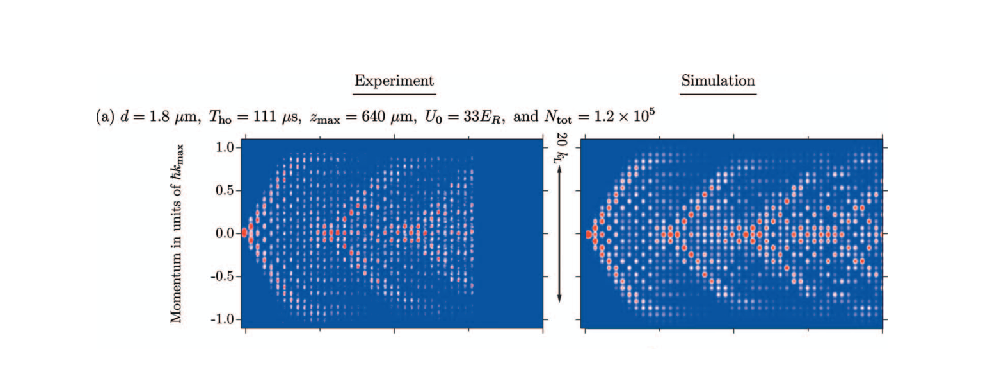
\includegraphics{Chapter6_secs/lattice_pulsing.pdf}
%     \caption{Fig.~1(a) of \cite{huckans2009quantum}. Concatenated absorption images of diffraction patterns, showing the evolving momentum distribution, compared with numerical GPE simulation results.}
%     \label{fig:lattice_pulsing}
% \end{figure*}

\subsection{Short term speckle pulsing}\label{short_pulse_sec}

To measure the PSD and the cutoff $k_c$ of the speckle potentials with short term speckle pulsing, we derive the evolution of the momentum states under two approximations. The first is the Raman-Nath approximation, atoms do not move far during the pulse.  The second is that the evolution time is short compared to $\hbar/V(x)$, so atoms do not acquire a phase comparable to $2\pi$.
Consider Hamiltonian
\begin{equation}
    \hat{H} = \frac{\hbar^2k^2}{2m} + V(x).
\end{equation}
The time evolution operator is
\begin{equation}
    \hat{U}(t) = \exp{-i\frac{\Delta t}{\hbar}\left[\frac{\hbar^2k^2}{2m}+V(x)\right]},
\end{equation}
Define $E_c$ as the energy associated with $k_c$, $\tau = \frac{\Delta t}{\hbar}E_c$, $\hat{k} = \frac{k}{k_c}$ and $S(x) = \frac{V(x)}{E_c}$
\begin{equation}
    \hat{U}(t) = \exp{-i\tau\left[\hat{k}^2+S(x)\right]}.
\end{equation}
Expand the operator to second order, 
\begin{equation}
    \hat{U}(t) = \exp{-i\tau\hat{k}^2/2}\exp{-i\tau S(x)}\exp{-i\tau\hat{k}^2/2}.
\end{equation}
We assume the initial state is $\ket{k=0}$, so the third term does not contribute. And we measure the distribution in $k$ space, so we can ignore the first term. The second term governs the short time evolution. To the lowest order, 
\begin{equation}
    \hat{U}(t)\ket{k=0} = \ket{k=0} - i\tau S(x) \ket{k=0}
\end{equation}
Expand $S(x)$ in $k$ space,
\begin{equation}
    S(x) = \sum_{k,k'}\Tilde{S}(k-k')\dyad{k}{k'}
\end{equation}
So
\begin{equation}
    \hat{U}(t)\ket{k=0} = \ket{k=0} - i\tau \sum_{\delta k}\Tilde{S}(\delta k)\ket{\delta k}
\end{equation}
The probability distribution of momentum states at time $\tau$ is
\begin{equation}\label{short_dist}
    P(k,\tau) = \tau^2 |\Tilde{S}(k)|^2 + \delta_{k,0}.
\end{equation}
It is proportional to the PSD of the speckle potential $|\Tilde{S}(k)|^2$ ignoring the central peak at $k=0$.

In the experiments, we put an iris right before the diffuser $D$ in \ref{fig:design}. By opening and closing the iris, we can control the size of the beam which determines $k_c$ of the speckle potential PSD in the focal plane. As the model we derived in Ch.~(\ref{speckle_chapter}) shows, the speckle beam size at the focal plane does not change with the beam size at the diffuser. The beam size at the focal plane is determined by the field-field correlation length at the diffuser. So the average speckle potential depth is proportional to the power of the beam which we can control when we change the size of the iris. 

We did the experiments for two iris sizes, $6.5\ {\rm mm}$ and $15\ {\rm mm}$, which correspond to $k_c=0.65k_r$ and $k_c=1.30k_r$, respectively. Here $k_r$ is defined with the largest recoil $k$ vector of atoms scattered by a $532\ {\rm nm}$ light beam focused by a one inch $f=30\ {\rm mm}$ lens. 
\begin{equation}
    k_r = \frac{2\pi}{532 {\rm nm}}\sin{\frac{\theta_{\rm R}}{2}}
\end{equation}
$\theta_{\rm R} \approx 45^\circ $ is shown in Fig.~(\ref{fig:raman_design}).
The average speckle potential match in both cases by controlling the power of the beam after the iris. 

We prepare BECs in a cross dipole trap, at $t=0$, we turn off the dipole trap and release the atoms for time-of-flight (TOF). Immediately after the dipole trap is turned off, we turn on the speckle beam and pulse for a short period of time, ranging from $20\ {\rm \mu s}$ to $250\ {\rm \mu s}$. After $18\ {\rm ms}$ TOF, we take absorption images of the atoms.

To compare with the experimental data, we simulate the process numerically. In the numerical simulation, we prepare the ground state of BECs in a dipole trap. At $t=0$, turn off the dipole trap and release the atoms. Immediately after, the speckle potential is turned on for a duration of $50\ {\rm \mu s}$ or $100\ {\rm \mu s}$, followed by free evolution for up to $20\ {\rm ms}$. We keep track of the momentum distribution of the atoms during the evolution. 

\begin{figure*}
    \centering
    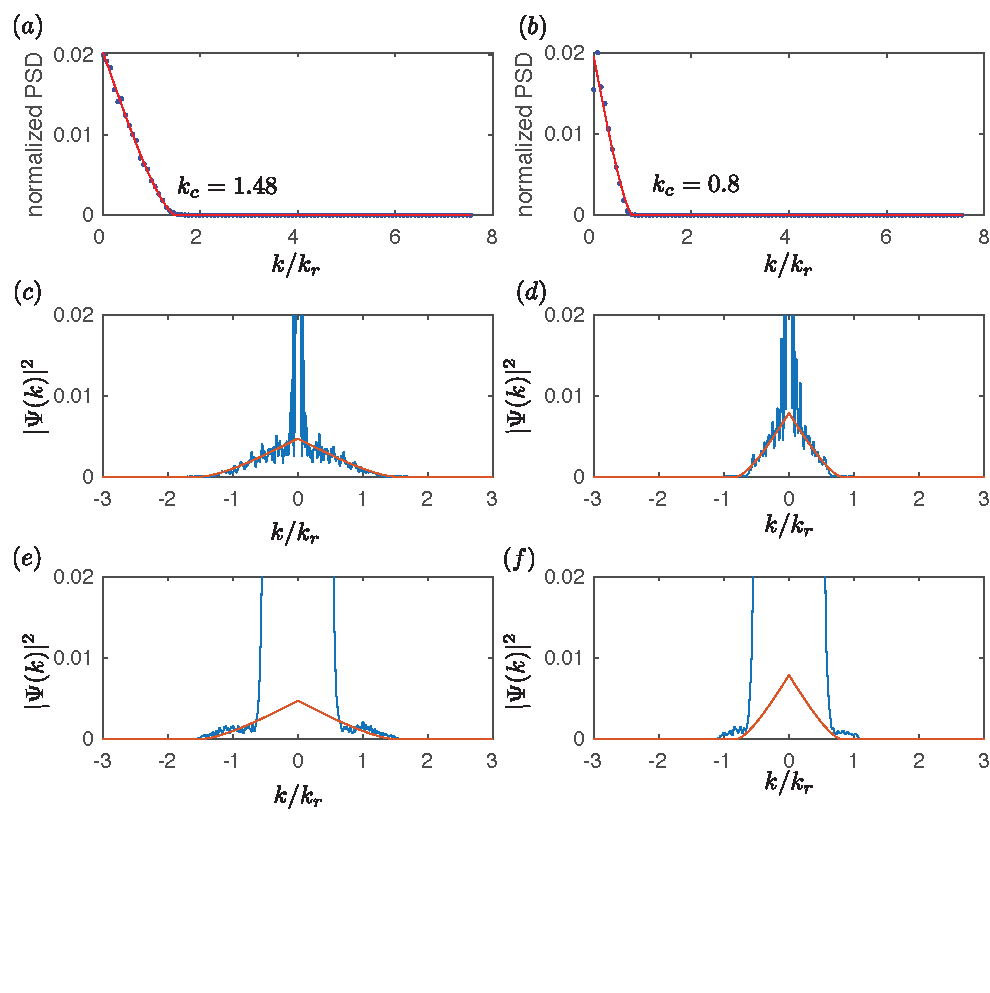
\includegraphics{Chapter6_secs/speckle_pulsing_simu.pdf}
    \caption{Simulation of short-term speckle pulsing. The left panel is for speckle potential with $k_c = 1.48k_r$, and the right panel for $k_c = 0.8k_r$. (a) and (b) verify the $k_c$ of both speckle potentials by plotting their PSD. (c) and (d) are the momentum distribution of atoms after released from the dipole trap and evolve under speckle pulses for $50\ {\rm \mu s}$. The red curves are proportional to the corresponding PSD of the speckle potential. The momentum distribution is an average of 20 speckle realizations. (e) and (f) are the momentum distribution of atoms after released from the dipole trap and evolve under speckle pulses for $50\ {\rm \mu s}$ followed by a $20\ {\rm ms}$ free expansion. The results are averaged over 20 speckle realizations. }
    \label{fig:speckle_pulsing_simu}
\end{figure*}

As Fig.~(\ref{fig:speckle_pulsing_simu}) shows, the simulation is done under two kinds of speckle potentials with different $k_c$ to compare with the experimental data. The left panel of Fig.~(\ref{fig:speckle_pulsing_simu}) is for the speckle potential with $k_c = 1.48k_r$ and the right panel for the speckle potential with $k_c = 0.80k_r$. Fig.~\ref{fig:speckle_pulsing_simu}(c) and Fig.~\ref{fig:speckle_pulsing_simu}(d) show the momentum distribution of atoms immediately after a $50\ {\rm \mu s}$ speckle pulsing, the results are averaged over 20 speckle realizations. The red curves are proportional to the PSD of the two kinds of speckle potentials, respectively. From Fig.~\ref{fig:speckle_pulsing_simu}(c) and Fig.~\ref{fig:speckle_pulsing_simu}(d) we can see the tail of the momentum distribution of atoms after short-term speckle pulsing matches with the PSD of the speckle potentials. The results agree with the analytical calculation of the momentum distribution in Eq.~(\ref{short_dist}), which predicts the momentum distribution to be a central $\delta$ function plus a tail that is proportional to the PSD of the speckle potentials. 

Fig.~\ref{fig:speckle_pulsing_simu}(e) and Fig.~\ref{fig:speckle_pulsing_simu}(f) show the momentum distribution of atoms after a $50\ {\rm \mu s}$ speckle pulse and a $20\ {\rm ms}$ time-of-flight (TOF). During the TOF, the mean-field expansion of the atoms broadens the momentum distribution. Both the central peak and the tail of the momentum distribution become broader after the TOF. In Fig.~\ref{fig:speckle_pulsing_simu}(f), for the speckle potential of smaller $k_c$, the tail of the momentum distribution is broadened more significantly. The broadened momentum distribution after TOF makes it harder to distinguish the speckle potentials with the tail of the momentum distribution.

\begin{figure*}
    \centering
    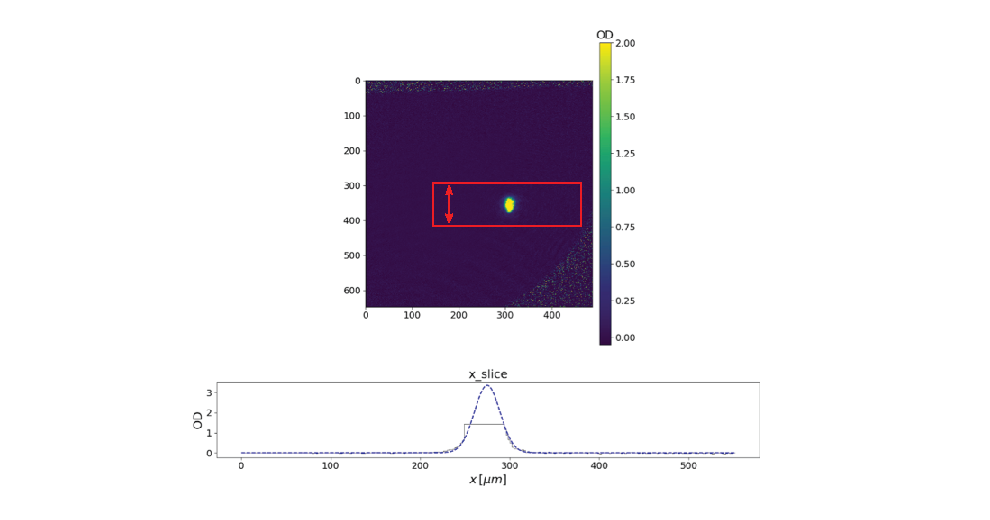
\includegraphics{Chapter6_secs/colOD.pdf}
    \caption{A sample of absorption images of atoms and analysis. The red square is a selected region of interest and the red arrow indicates the direction we take average. The masked and averaged spatial distribution of atoms (black curve) and a fitted Gaussian curve (blue dashed) are plotted below.}
    \label{fig:colOD}
\end{figure*}

\begin{figure*}
    \centering
    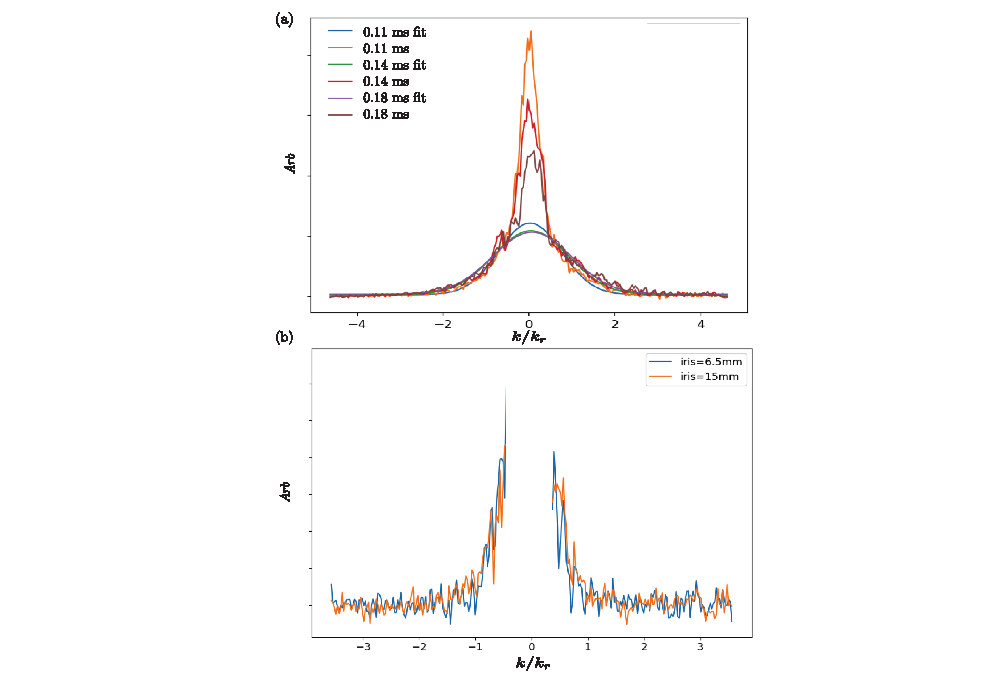
\includegraphics{Chapter6_secs/short_pulse.pdf}
    \caption{Momentum distribution after short-term speckle pulses and $18\ {\rm mm}$ TOF. (a). A few samples of momentum distribution of atoms without mask, along with fitted Gaussian curves to the masked momentum distribution. (b). The tails of the momentum distribution after short-term pulses of speckle potential with different PSD. The PSD of the speckle potentials are controlled by the iris sizes and the results are averaged for speckle pulsing time ranging from $80\ {\rm \mu s}$ to $150\ {\rm \mu s}$.}
    \label{fig:short_pulse}
\end{figure*}


Fig.~\ref{fig:colOD} and Fig.~\ref{fig:short_pulse} show the analysis results of the absorption images after TOF for two kinds of speckle potentials generated with different iris sizes. During TOF, the momentum distribution of atoms is mapped to their spatial distribution. From the absorption images, we can compute the momentum distribution from the spatial profile of the atoms. In the analysis, from the absorption images of atoms after TOF shown in Fig.~\ref{fig:colOD}, we select a region of interest around the center of the atoms indicated by the red square. And compute the average spatial distribution of atoms along the horizontal direction (red arrow). The central peak of this average spatial distribution is masked to show the detail of the tails. Fig.~\ref{fig:colOD} shows an example of the masked averaged spatial distribution along $x$ direction (black curve) and a Gaussian fit (blue dashed curve). The resultant tails of the spatial distribution are averaged over short-term speckle pulsing duration ranging from $80\ {\rm \mu s}$ to $150\ {\rm \mu s}$. The tails of the spatial distribution are then converted to that of the momentum distribution in a unit of $k_r$. 


Fig.~\ref{fig:short_pulse}(a) shows a few samples of the averaged momentum distribution along $x$ direction without a mask for short-term speckle pulsing, along with fitted Gaussian curves to the masked momentum distribution. From Fig.~\ref{fig:short_pulse}(a) we can see it is necessary to mask the central peak of the momentum distribution in order to analyze the width of the tails. Fig.~\ref{fig:short_pulse}(b) is the momentum distribution of atoms after short-term pulses of speckle potentials with different PSD, averaged over pulsing duration ranging from $80\ {\rm \mu s}$ to $150\ {\rm \mu s}$. From Fig.~\ref{fig:short_pulse}(b), it is hard to tell the difference between the two curves for two reasons. First, in the absorption images, the signal-noise-ratio at the tails of the density profile is low. Just by taking the average, it is hard to reduce the noise and see the clear tails as in the numerical simulation in Fig.~\ref{fig:speckle_pulsing_simu}. Second, as the simulation results show in Fig.~\ref{fig:speckle_pulsing_simu}(e) and Fig.~\ref{fig:speckle_pulsing_simu}(f), during TOF, the mean-field expansion broadens the momentum distribution more significantly for speckle pulsing with smaller $k_c$. So the width of the tails of the momentum distribution for the pulsing of two kinds of speckle potentials is closer to each other after TOF than before. For the two reasons, we conclude we can not quantitatively measure the $k_c$ of the speckle potential by using the absorption images after short-term speckle pulsing and TOF.



\subsection{Long term speckle pulsing}\label{long_pulse}

In the experiments, it is important to know the average speckle potential at the atoms. But unfortunately, it is hard to measure the power of the speckle beam directly at the atoms and infer the average speckle potential. Because in the experiments, we can not put a power meter anywhere we want to measure the power of the beam. And besides, it is the intensity that matters, and we don't have perfect knowledge of the beam size at the atoms. After the closest point to the vacuum glass cell where we can use a power meter to measure the power, the beam goes through lenses, reflected by mirrors, glass cell or even dichroic mirrors. The power of the beam decreases at each of the optical element. To the best of our knowledge, for the previous experiments using speckle beams, the average speckle potential was not measured directly. It could be inferred by calculating the power given the power loss at each optical element. Or the power could be measured for an identical speckle beam set up on the test bench and it is assumed the power at the atoms is the same as the power of the test speckle beam in the focal plane. 

Inspired by \cite{huckans2009quantum}, we obtained the mean potential depth by making the atoms evolve under the speckle beam pulses. Compared with \cite{huckans2009quantum}, for $t \gg t_{RN}$, we do not expect to see the collapse and revive phenomenon due to the anharmonicity of the speckle potential. Instead, at long speckle pulsing time, the momentum distribution should reach equilibrium and by virial theorem, the average stationary kinetic energy is half of the average total energy which is the initial average speckle potential. 

To confirm our understanding, we did numerical simulations of the long-term speckle pulsing. Fig.~\ref{fig:speckle_pulsing} shows the simulation and experimental results of the speckle pulsing for the pulsing duration up to $2\ {\rm ms}$. In the simulation, we release the BECs from the dipole trap and immediately turn on the speckle potential. The atoms evolve under the speckle potential and we keep track of the width of the momentum distribution. We did the simulation for different average speckle potential depth ranging from $0\ {\rm Hz}$ to $1600\ {\rm Hz}$, with a $200\ {\rm Hz}$ spacing. The results are shown as the nine curves, each one is averaged over 20 speckle realizations. When the average speckle potential is zero, the width of the momentum distribution increases driven by the mean-field expansion. From the simulation results shown in Fig.~\ref{fig:speckle_pulsing}(a), the width of the momentum distribution increases rapidly after the speckle potential is turned on and becomes stationary after around $0.25\ {\mu s}$. The stationary width increases with the average speckle potential depth. Fig.~\ref{fig:speckle_pulsing}(b) shows the experimental results. In the experiment, we release the atoms from the dipole trap, pulse the speckle potential for up to $2\ {\rm mm}$ followed by TOF. The total time for the speckle pulsing and the TOF is $18\ {\rm ms}$, a constant for different pulsing duration. We take the absorption images after TOF and fit a Gaussian function to the density profile of the atoms. Fig.~\ref{fig:speckle_pulsing}(b) shows the width of the fitted Gaussian function vs the duration of the speckle pulses. The Gaussian width increases with the pulsing duration in short term and becomes stationary after around $0.25\ {\rm ms}$, which is consistent with the simulation results. 

\begin{figure*}
    \centering
    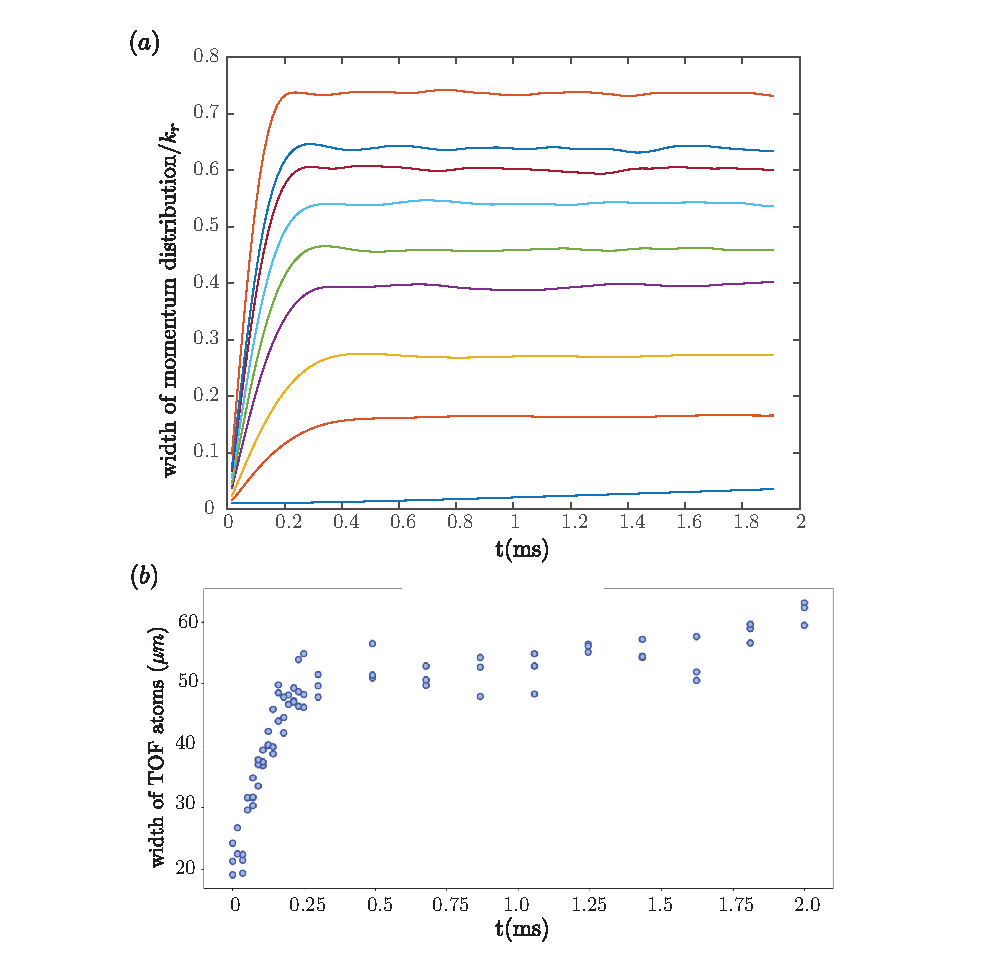
\includegraphics{Chapter6_secs/speckle_pulsing_width.pdf}
    \caption{The simulation and the experiments of the speckle beam pulsing. (a). The width of the momentum distribution of atoms evolving under the speckle potentials of different potential depth ranging from $0$ to $1600\ {\rm Hz}$.  (b). The Gaussian width of atoms in the absorption images after TOF for different speckle pulsing duration.}
    \label{fig:speckle_pulsing}
\end{figure*}

To infer the average speckle potential from the width of the momentum distribution after long-term speckle pulsing, we compute the average kinetic energy using the fitted Gaussian width of the density profile of atoms after TOF.
\begin{equation}
    \langle \hat{K} \rangle = \frac{1}{2} m \left(\frac{\sigma}{\tau}\right)^2
\end{equation}
Here $\tau$ is the time for TOF. The average speckle potential is equal to the average total energy, which by virial theorem is twice the average kinetic energy. In Fig.~\ref{fig:avg_speckle_poten}(b), the computed total energy is plotted against a photo diode (PD) reading. In our experiments, we use a pick-off mirror to reflect a fixed percentage of the power of the speckle beam to a PD and the reading of the PD in Volt is proportional to the power of the beam at the atoms. We fit a line crossing the origin to the data, by reading the PD we have an estimate of the average speckle potential at the atoms. 

To compare with the experimental results, we also did numerical simulations. In the simulations, we release the atoms from the dipole trap at $t=0$ and pulse the speckle potential for $1\ {\rm ms}$ followed by a $20\ {\rm ms}$ free evolution. The simulations are done with two kinds of speckle potentials, $k_c=0.80k_r$ and $k_c=1.48k_r$, respectively. For each kind of the speckle potential, the average potential depth ranges from $0\ {\rm Hz}$ to $1600\ {\rm Hz}$ with a $200\ {\rm Hz}$ spacing. We compute the momentum distribution and the average kinetic energy at the end of the free evolution. The average total energy is twice the average kinetic energy deducted by the mean-field energy computed from the average kinetic energy in the no-pulsing case. And the resultant average total energy is plotted against the known average potential depth. In agreement with our prediction, the curves are close to the diagonal line (dashed) for both kinds of speckle potentials.


\begin{figure*}
    \centering
    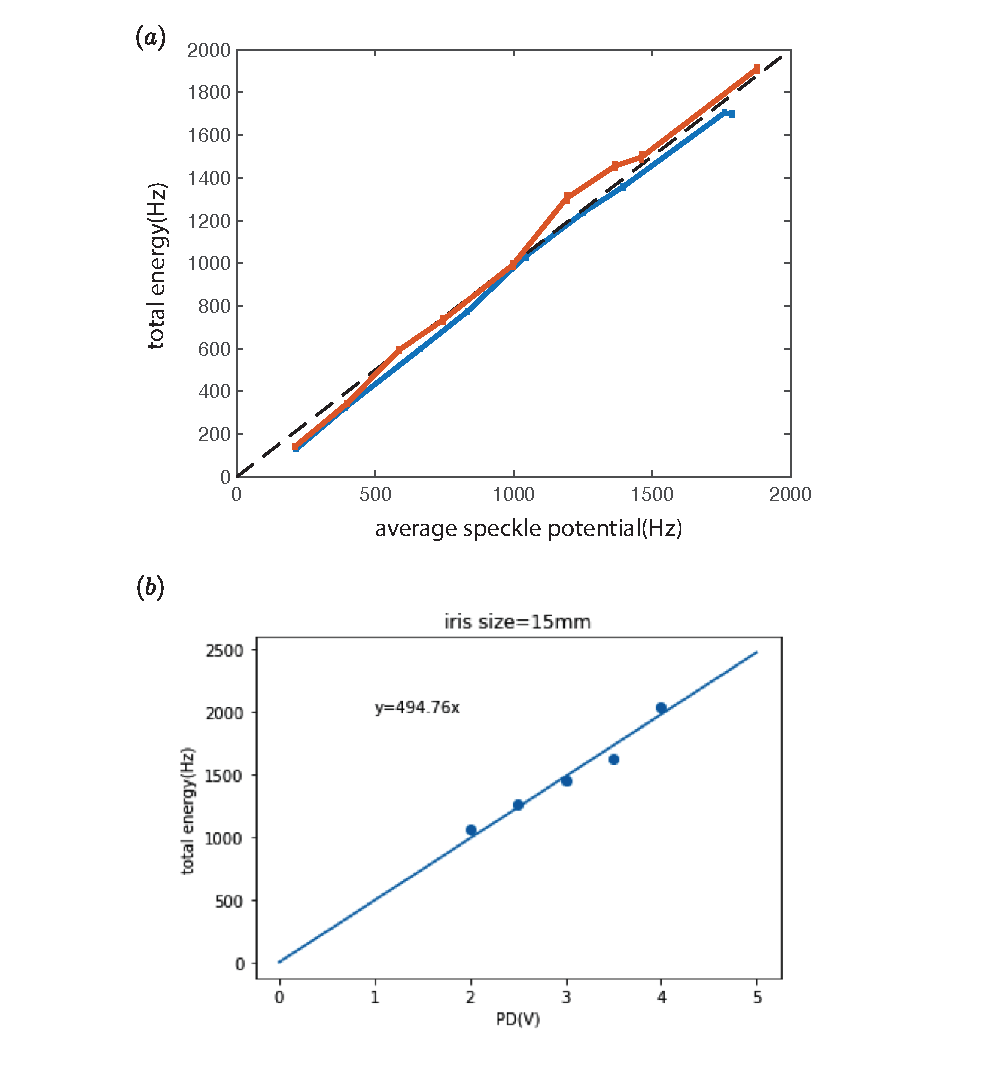
\includegraphics{Chapter6_secs/average_speckle_potential.pdf}
    \caption{Calibration of the average speckle potential depth. (a). In the numerical simulation, the average total energy inferred from the momentum distribution after $20\ {\rm ms}$ free evolution is plotted against the known average speckle potential depth. The red curve and the blue curve are for the speckle potentials with $k_c = 0.80k_r$ and $k_c=1.48k_r$, respectively. The dashed line is diagonal. (b). In the experiment, the average total energy computed from long-term speckle pulsing data is plotted against the PD reading.}
    \label{fig:avg_speckle_poten}
\end{figure*}




\section{Transport of spinless BECs in speckle potentials}\label{transport}

In Ch.~(\ref{chpt 5}), we study the transport of spinless BECs under speckle potentials. As Fig.~(\ref{fig:single}) shows, a BEC with a chemical potential $\sim 300\ {\rm Hz}$ travels through speckle potentials with average potential depth $\sim 200\ {\rm Hz}$, could be scattered by the speckle potential and decelerate. The deceleration of a BEC depends on its initial velocity, the speckle potential depth, and the cutoff $k_c$ in the speckle potential PSD. As Fig.~\ref{fig:single}(d) shows, after evolving under the speckle potentials for $16\ {\rm mm}$, the BECs with small initial velocity has more significant deceleration. For BECs with large initial velocity, $k_0>k_c/2$, the deceleration is minimal during the $16\ {\rm mm}$.

In the experiments, we study how BECs with different velocities decelerate. As discussed in Ch.~(\ref{speckle_chapter}), we can make speckle potentials that have the same PSD as the ones we use in our numerical simulations. And as discussed in Sec.~(\ref{speckle_pulsing}), the average speckle potential depth can be inferred from a PD reading. So an ideal experimental sequence is to have the BEC travel with constant velocity under well-calibrated speckle potential, and the final velocity would be measured by using $insitu$ or TOF absorption images. To that end, the first challenge we are faced with is that how to make a BEC travel with a constant velocity for an extensive amount of time ($16\ {\rm mm}$ in the simulation). We make BECs by doing evaporative cooling in a cross dipole trap as discussed in Sec.~(\ref{dipole trap}), so our first choice is to make BECs travel in the cross dipole trap. As Eq.~(\ref{dipole_poten}) suggests, dipole potential is proportional to the intensity of the dipole beam. 

In our case, as discussed in \ref{speckle_design}, we image atoms in $z$ direction and measure the motion of atoms in $x$ direction. The dipole potential in $x$ direction is a combination of the dipole potential from $z$ dipole beam and $x$ dipole beam. The width of the dipole potential from $x$ dipole beam is the Rayleigh range, which in our case is $\sim 1.3\ {\rm mm}$. Based on our design, the velocity of atoms corresponds to the recoil $k$ vector $k_r$ is $3.3\ {\rm \mu m/ms}$. We expect the atoms to move less than $50\ {\rm \mu m}$ during the experiment, so the dipole potential from x dipole beam can be ignored.

In $x$ direction, the dipole potential from the $z$ dipole beam is
\begin{equation}
    V_{dip}(x) = -V_0\exp{-\frac{2x^2}{w^2}}.
\end{equation}
where $w$ is the width of the beam at the atoms. Expand the potential at $x=0$ to second order,
\begin{equation}
    V_{dip}(x) \approx -V_0 + \frac{2V_0}{w^2}x^2,
\end{equation}
has a quadratic form. Around the center of the trap, the dipole potential can be approximated by a harmonic potential with frequency $\sqrt{\frac{4V_0}{w^2}}$.

In the ideal case, the atoms would move at a constant velocity in the dipole trap, meaning the frequency $\sqrt{\frac{4V_0}{w^2}}$ is zero and the $z$ dipole beam is completely turned off. More realistically, if the velocity of the atoms change by less than 5\% at the center of the trap in $15\ {\rm ms}$, the period of the harmonic oscillation needs to be more than $300\ {\rm ms}$. So the trapping frequency is around $3\ {\rm Hz}$. 

The $x$ dipole beam and the $z$ dipole beam in our experiments are the first order and zeroth-order beams from an AOM, the total power of the two beams are conserved. We optimized the ratio of the power of the two beams to maximize the phase space density of the BECs after the dipole evaporation stage. In the optimized case, the measured trapping frequency in $x$ direction is $21\ {\rm Hz}$. In order to decrease the $x$ trapping frequency, we need to allocate more power in the $x$ dipole beam and less in the $z$ dipole beam. But in the process of decreasing the $x$ trapping frequency, a few problems occurred. 

Fig.~\ref{fig:lower trapping freq} shows the BEC with $x$ trapping frequency of $21\ {\rm Hz}$ compared with the BEC with $x$ trapping frequency of $5.8\ {\rm Hz}$. Compared with the BEC in Fig.~\ref{fig:lower trapping freq}(a), the BEC in Fig.~\ref{fig:lower trapping freq}(b) is stretched in the $x$ direction due to small trapping frequency. The signal is much weaker and the large length in $x$ direction makes it hard to accurately detect the center of the atoms and the center-of-mass motion.

\begin{figure*}
    \centering
    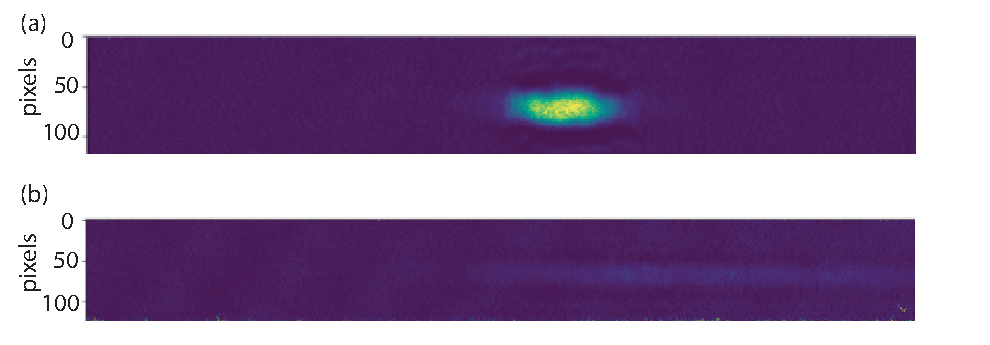
\includegraphics{Chapter6_secs/decrease_trap_freq.pdf}
    \caption{$insitu$ absorption images of BECs with different dipole parameters. (a) A BEC with $x$ trapping frequency of $21\ {\rm Hz}$. (b) A BEC with $x$ trapping frequency of $5.8\ {\rm Hz}$}
    \label{fig:lower trapping freq}
\end{figure*}

Alternatively, we can keep the current dipole trap configuration and decrease the time that BECs travel under speckle potentials. We hope to find the duration of the speckle potential pulses that is as short as possible, but its deceleration effect on the BECs is still significant for speckle potential weak enough not to cause trapping effect. 

In Fig.~\ref{fig:deceleration_in_dip_osc}, the blue dots show the oscillation of a BEC in $x$ direction in a dipole trap with $x$ trapping frequency $21\ {\rm Hz}$. The center of the atoms is measured from $insitu$ images of atoms. At the center of the dipole trap, the atoms are at the maximum velocity $v_0$, $mv_0/\hbar = 1.8k_r$. The first time the atoms reach maximum velocity is at $21\ {\rm ms}$. We make the atoms do the same dipole oscillation as the blue dots show, at $21\ {\rm ms}$, we turn on the speckle potential and hold for $1\ {\rm ms}$. After $1\ {\rm ms}$, the speckle potential is turned off and we track the center-of-mass motion of the atoms in $x$ direction in the dipole trap. The center-of-mass motion of atoms after the speckle pulse is shown as the orange dots in Fig.~\ref{fig:deceleration_in_dip_osc}. 

\begin{figure*}
    \centering
    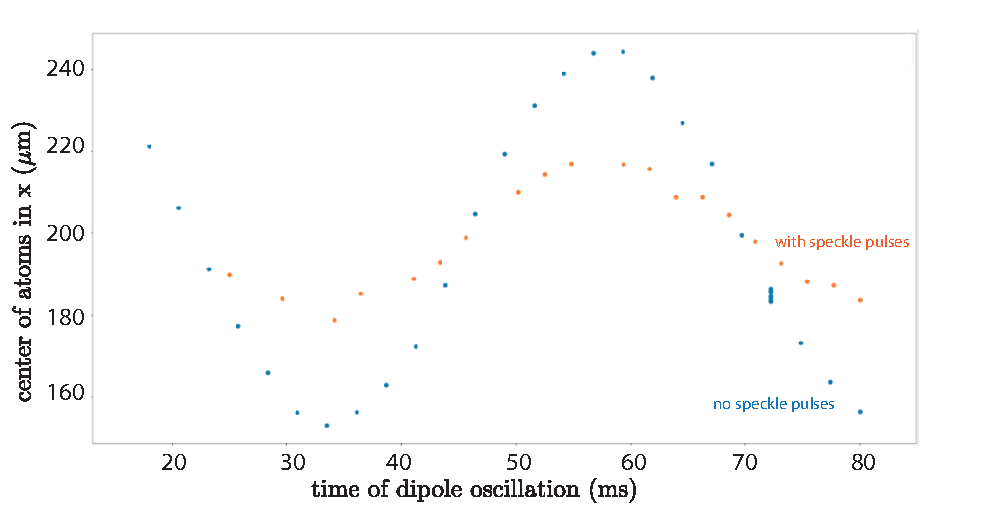
\includegraphics{Chapter6_secs/deceleration_in_dip_osc.pdf}
    \caption{Center-of-mass motion in $x$ direction of atoms during dipole oscillation. The blue dots show a full cycle of dipole oscillation without pulses of the speckle potentials. The orange dots show the dipole oscillation of atoms with the same initial velocity as the blue dots show, but with a $1\ {\rm ms}$ speckle pulse at $21\ {\rm ms}$. The average speckle potential depth is $\approx 640\ {\rm Hz}$.}
    \label{fig:deceleration_in_dip_osc}
\end{figure*}

The amplitude of the oscillation shown by the orange dots is smaller than the amplitude shown by the blue dots. We fit a sinusoidal function to both and infer the velocities of the atoms at $t=21\ {\rm ms}$. Without the pulse of speckle potential at $t=21\ {\rm ms}$, the velocity of the atoms is $v_0$, $mv_0/\hbar = 1.8k_r$. With the pulse, the velocity of the atoms is $v_f$, $mv_f/\hbar = 0.7k_r$. This measurement demonstrated that a speckle potential pulse with an average potential depth of $\approx 640\ {\rm Hz}$, can have a significant deceleration effect on atoms within $1\ {\rm ms}$. This allows us to measure the deceleration of atoms evolving in speckle potentials in our optimized dipole trap, without having to reduce the $x$ trapping frequency.

Using this method, we measured the deceleration of atoms at different velocities $v_0$ after pulses of speckle potential for $1\ {\rm ms}$ with an average potential depth of $\approx 500\ {\rm Hz}$. Fig.~\ref{fig:spinless transport} shows the experimental measurements compared with the numerical simulation results. The red circles in Fig.~\ref{fig:spinless transport} show the experimental results. In the numerical simulations, we make atoms with different initial velocities evolve under speckle potentials with different potential depth for $1\ {\rm ms}$ and measure the final velocities. The initial velocities range from $0.2\frac{\hbar k_r}{m}$ to $2.2\frac{\hbar k_r}{m}$. The blue curve and the yellow curve in Fig.~\ref{fig:spinless transport} correspond to speckle potential depth of $500\ {\rm Hz}$ and $800\ {\rm Hz}$, respectively. In the experiments, the average speckle potential depth is inferred from Fig.~\ref{fig:avg_speckle_poten}. As discussed in Sec.~\ref{long_pulse}, we use the stationary width of the momentum distribution after long-term speckle pulses to measure the average speckle potential. Here the deceleration measurement is done with a PD reading of $1.0\ {\rm V}$, which corresponds to an average speckle potential of $\approx 500\ {\rm Hz}$. For initial velocities $v_0$, the measured final velocities $v_f = \frac{\hbar k_r}{m}$ are lower than the final velocities in the simulation with average speckle potential of $500\ {\rm Hz}$, and are close to those in the simulation with average speckle potential of $800\ {\rm Hz}$. There are a few potential causes that can lead to the gap. First, in the measurements of the stationary width of momentum distribution after long-term pulses of speckle potential shown in Fig.~\ref{fig:avg_speckle_poten}, the stationary width is noisy which leads to uncertainty in the calculation of average speckle potential depth. Second, as discussed in Sec.~\ref{short_pulse_sec}, it is hard to measure the $k_c$ of the optical speckle potentials used in the experiments accurately. The difference in $k_c$ of speckle potentials used in the simulations and the experiments can also lead to this gap.

%we fit a Gaussian function to the spatial distribution of atoms to extract the center-of-mass positions, as the dots in Fig.~\ref{fig:deceleration_in_dip_osc} show. Then we fit a sinusoidal function to the center-of-mass positions of atoms when they oscillate in a dipole trap, and infer the velocity at $t=21~{\rm ms}$. The Gaussian fits and the inference of velocities from the sinusoidal fits also introduce uncertainties.

\begin{figure*}
    \centering
    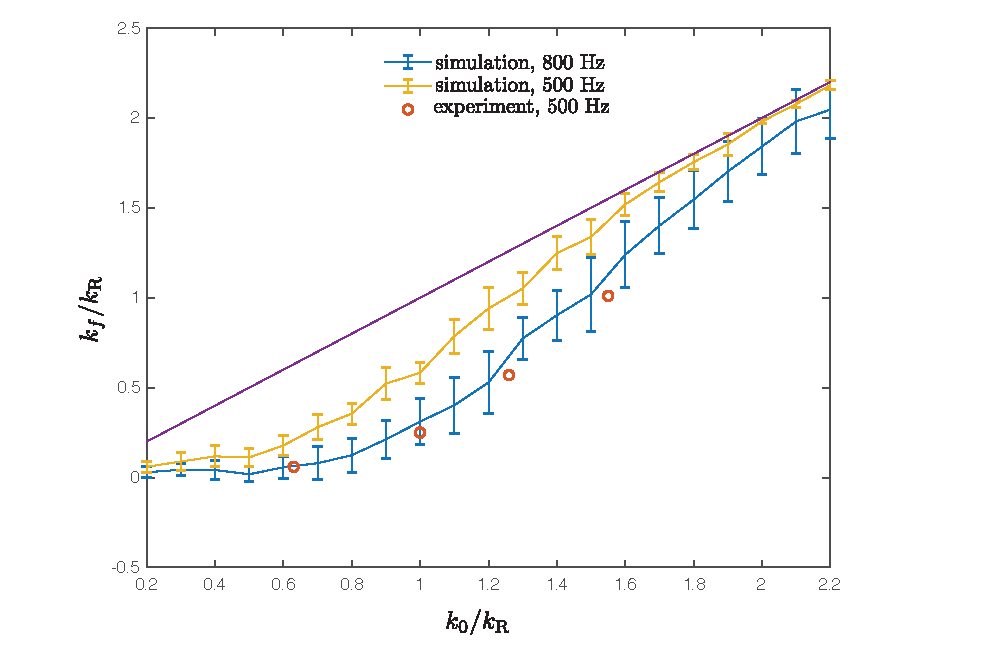
\includegraphics{Chapter6_secs/spinless_transport.pdf}
    \caption{Deceleration of atoms after a $1\ {\rm ms}$ pulse of the speckle potentials. The red circles are the results of measurements in the experiments. The average speckle potential depth inferred from the photo diode reading is $\approx 500\ {\rm Hz}$. The blue curve and the yellow curve are the results of numerical simulations. The blue curve is the final velocities vs the initial velocities after evolving under speckle potentials with average potential depth of $800\ {\rm Hz}$, and the yellow curve is for speckle potential with average potential depth of $500\ {\rm Hz}$. Both the blue curve and the yellow curve are averaged over 20 speckle realizations and the error bars show the standard deviations. The purple line is diagonal. }
    \label{fig:spinless transport}
\end{figure*}
%\renewcommand{\thechapter}{2}

\chapter{Laser cooling and trapping of neutral atoms}

The Nobel Lecture of W.D.Phillips, {\it Laser cooling and trapping of neutral atoms} \cite{phillips1998nobel} tells a great story of the development of laser cooling techniques since the late 1970s. It is recommended for readers who want to learn not only the development of the laser cooling research field but also how researchers approach new physics and technology in a close view. It is aspiring to learn the mature technology that cold atom researcher uses on a daily basis to expand the boundary of physics results from the intelligence, efforts, and persistent pursuit of the early generation of physicists.    

Laser cooling techniques eventually lead to the observation of BEC in 1995, the first Bose-Einstein condensate was created by Eric Cornell, Carl Wieman, and co-workers at JILA on 5 June 1995 \cite{anderson1995observation}. They cooled a dilute vapor of approximately two thousand $^{87} {\rm Rb}$ atoms to below 170~ ${\rm nK}$ using a laser cooling and magnetic evaporative cooling. About four months later, an independent effort led by Wolfgang Ketterle at MIT condensed $^{23} {\rm Na}$ \cite{davis1995bose}. The observation of BEC won laser cooling pioneers Steven Chu, Claude Cohen-Tannoudji, and William D. Phillips the 1997 Nobel Prize in Physics. And Cornell, Wieman, and Ketterle won the 2001 Nobel Prize in Physics for their achievements.

After more than twenty years, the research field of cold atoms is prosperous. The development of laser cooling techniques and the methods to make stable BEC have not only achieved a new state of matter predicted only by Quantum physics, the highly controllable optical and magnetic potential, tunable interaction between particles, and precision measurement techniques have made the BEC system a great platform for Quantum simulation and Quantum computation. 

In this chapter, we use $^{87} {\rm Rb}$ as an example. Start from its energy level, its interaction with light and magnetic field, and then discuss the laser cooling techniques that are essential to make BEC.  

\section{Hyperfine Structures}

\subsection{Energy Level Splitting}
The energy splitting of $^{87} {\rm Rb}$ ground state and the first excited state can be found in Fig.~(\ref{fig:D1andD2}) from \cite{steck2001rubidium}, it is a great source of $^{87} {\rm Rb}$ D lines data.

For the ground state of $^{87} {\rm Rb}$, the quantum number of orbital angular momentum ${\bf L}$ is 0 and the first excited state $L = 1$. When we consider the spin of the single electron in the outer shell of the atom, $S = 1/2$, and the interaction between spin and orbital angular momentum ${\bf L} \cdot {\bf S}$, the excited state splits into a fine-structure doublet. The eigenvalue of total electron angular momentum 
\begin{equation}
    {\bf J} = {\bf L} + {\bf S}    
\end{equation}
becomes a good quantum number. For the ground state,  $L = 0$, $S = 1/2$, and $J = 1/2$. The ground state is labeled as $5^2S_{1/2}$ where the atomic states are described by term symbols of the form
\begin{equation}
    ^{2S+1}L_J.
\end{equation}
The interaction between the spin and the orbital angular momentum splits the excited state into doublet $5^2P_{1/2}$ and $5^2P_{3/2}$. The transition between the ground state and the excited state is split into two lines, D1 line($5^2S_{1/2} \rightarrow 5^2P_{1/2}$) and D2 line ($5^2S_{1/2} \rightarrow 5^2P_{3/2}$).

Accounting for nuclear angular momentum ${\bf I}$, the states further split into hyperfine states and are represented in the basis of the total angular momentum
\begin{equation}
    {\bf F} = {\bf J} + {\bf I}.    
\end{equation}
The quantum number of the nuclear spin of $^{87} {\rm Rb}$ is 3/2, as shown in Fig.~(\ref{fig:D1andD2}), the $^{87} {\rm Rb}$ ground state $5^2S_{1/2}$ splits into hyperfine states $\ket{F=1}$ and $\ket{F=2}$. The excited state $5^2P_{1/2}$ splits into hyperfine states $\ket{F=1}$ and $\ket{F=2}$. And the excited state $5^2P_{3/2}$ splits into hyperfine states $\ket{F=1}, \ket{F=2},\ket{F=3}$ and $\ket{F=4}$. The Hamiltonian that leads to the hyperfine split consists of magnetic dipole interaction and electric quadrupole interaction,
\begin{equation}
    \hat{H}_{hfs} = A_{hfs}{\bf I}\cdot{\bf J} + B_{hfs}\frac{3({\bf I}\cdot{\bf J})^2 + 3/2{\bf I}\cdot{\bf J} - I(I+1)J(J+1)}{2I(2I-1)2J(2J-1)}.
\end{equation}
Here $A_{hfs}$ is the magnetic dipole constant and $B_{hfs}$ is the electric quadrupole constant. The hyperfine energy splits for the states are
\begin{equation}
    \Delta E_{hfs} = \frac{1}{2}A_{hfs}K + B_{hfs}\frac{3/2K(K+1) - 2I(I+1)J(J+1)}{2I(2I-1)2J(2J-1)}
\end{equation}
where 
\begin{equation}
    K = F(F+1) - I(I+1) - J(J+1).
\end{equation}
The numerical results of hyperfine states energy can be found in Fig.~(\ref{fig:D1andD2}), they are calculated given the experimental measurement of $A_{hfs}$ and $B_{hfs}$ \cite{bize1999high,ye1996hyperfine,barwood1991frequency}.
\begin{figure}[htbp]
    \centering
    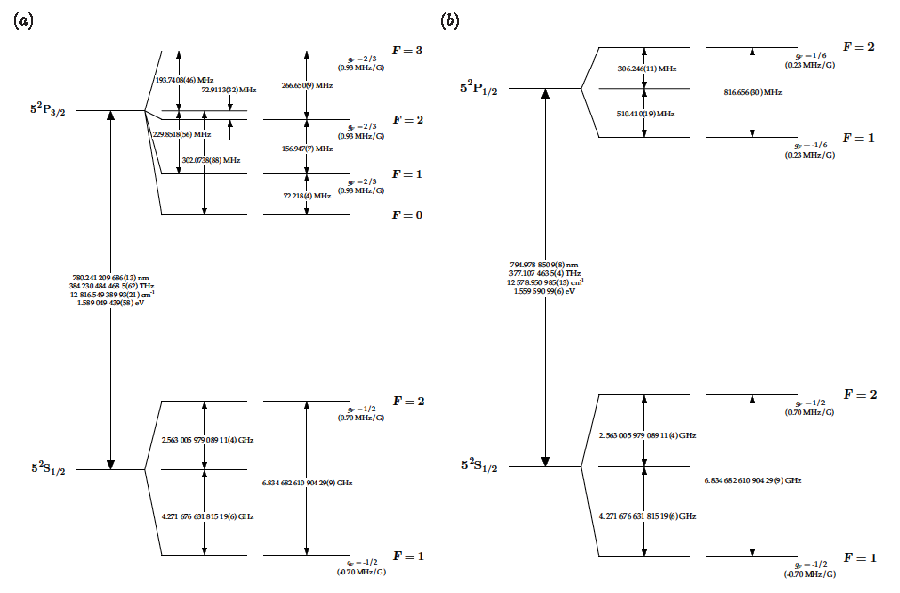
\includegraphics[width=\textwidth]{Chapter2_secs/D1andD2.pdf}
    \caption{Energy splitting of the $^{87} {\rm Rb}$ ground state and the first excited state. }
    \label{fig:D1andD2}
\end{figure}
\subsection{Zeeman splitting of $^{87} {\rm Rb}$ hyperfine ground states}\label{zeeman chpt}
The angular momentum of $^{87} {\rm Rb}$ interacts with the external magnetic field and the hyperfine states split into sub-states. Here we use perturbation theory to calculate the energy of each sub-states of $^{87} {\rm Rb}$ ground state.

For the $^{87} {\rm Rb}$ ground state, $J=1/2$ and $I=3/2$. It has hyperfine states $\ket{F=1}$ and $\ket{F=2}$. The Hamiltonian with external magnetic field is 
\begin{equation}
    \hat{H} = \hat{H}_{hfs} + (\mu_B g_J\Vec{J} + \mu_N g_I\Vec{I})\Vec{B}.
\end{equation}
Here $\mu_B = 9.27\times 10^{-24} {\rm J}\cdot {\rm T}^{-1}$ is Bohr magneton, the natural unit for expressing the magnetic moment of an electron caused by either its orbital or spin angular momentum. $\mu_N = 5.05\times 10^{-27} {\rm J}\cdot {\rm T}^{-1}$ is the nuclear magneton. $g_J$ and $g_I$ are land\'e g-factors. For $^{87} {\rm Rb}$ ground state, $g_J \approx 2.00233$ and $g_I \approx -0.00099$. 

Define the direction of magnetic field z, the Hamiltonian can be represented by the z-component of angular momentum
\begin{equation}
    \hat{H} = \hat{H}_{hfs} + \mu_B(g_J m_J + g_Im_I)B,
\end{equation}
where $m_J$ and $m_I$ are magnetic quantum numbers. $\hat{H}_{hfs}$ is diagonal in the basis of $\{\ket{F,m_F}\}$, and we can proceed by representing states $\ket{J=1/2,m_J,I=3/2,m_I}$ with $\{\ket{F,m_F}\}$ and calculate the energy of states $\ket{F,m_F}$ to second order.

\begin{align}
    &\ket{\frac{1}{2},\frac{3}{2}} = \ket{2,2}, &&\ket{\frac{1}{2},\frac{1}{2}} = \frac{\sqrt{3}}{2}\ket{2,1} - \frac{1}{2}\ket{1,1}\\\nonumber
    &\ket{\frac{-1}{2},\frac{3}{2}} = \frac{1}{2}\ket{2,1} + \frac{\sqrt{3}}{2}\ket{1,1}, &&\ket{\frac{-1}{2},\frac{1}{2}} = \frac{1}{\sqrt{2}}\ket{2,0} + \frac{1}{\sqrt{2}}\ket{1,0}\\ \nonumber
    &\ket{\frac{1}{2},\frac{-1}{2}} = \frac{1}{\sqrt{2}}\ket{2,0} - \frac{1}{\sqrt{2}}\ket{1,0}, &&\ket{\frac{1}{2},\frac{-3}{2}} = \frac{1}{2}\ket{2,-1} - \frac{\sqrt{3}}{2}\ket{1,-1}\\ \nonumber
    &\ket{\frac{-1}{2},\frac{-1}{2}} = \frac{\sqrt{3}}{2}\ket{2,-1} - \frac{1}{2}\ket{1,-1}, &&\ket{\frac{-1}{2},\frac{-3}{2}} = \ket{2,-2}\\ \nonumber
\end{align}

In the $\{\ket{F,m_F}\}$ basis,
\begin{equation}
    \hat{H}_{hfs}\ket{F,m_F} = E_{F}\ket{F,m_F}.
\end{equation}
Treat the interaction with the external magnetic field as a perturbation, the first-order perturbed energy for state $\ket{F,m_F}$ is
\begin{equation}
    \Delta E_1 = \matrixel{F,m_F}{(g_J\Vec{J}_z + g_I\Vec{I}_z)}{F,m_F}\mu_B B,
\end{equation}
and the second order perturbed energy is
\begin{equation}
    \Delta E_2 = \sum_{F',m_F'} \frac{|\matrixel{F,m_F}{(g_J\Vec{J}_z + g_I\Vec{I}_z)}{F',m_F'}|^2}{E_F-E_{F'}}(\mu_B B)^2.
\end{equation}

The energy of $\ket{F,m_F}$ states are listed here, in the units of ${\rm MHz}$, ${\rm MHz/G}$ and ${\rm MHz/G^2}$. The numbers are useful for quick estimation of the magnetic field in the lab.
\begin{align}
    \ket{2,2} &= 2.75\times 10^3h ~{\rm MHz} + 1.405h~{\rm MHz/G}\times B + 0h ~{\rm MHz/G^2}\times B^2\\\nonumber
    \ket{2,1} &= 2.75\times 10^3h ~{\rm MHz} + 0.7026h~{\rm MHz/G}\times B + 2.879\times 10^{-4}h ~{\rm MHz/G^2}\times B^2\\\nonumber
    \ket{2,0} &= 2.75\times 10^3h ~{\rm MHz} + 0h~{\rm MHz/G}\times B + 3.839\times 10^{-4}h ~{\rm MHz/G^2}\times B^2\\\nonumber
    \ket{2,-1} &= 2.75\times 10^3h ~{\rm MHz} - 0.7026h~{\rm MHz/G}\times B + 2.879\times 10^{-4}h ~{\rm MHz/G^2}\times B^2\\\nonumber
    \ket{2,-2} &= 2.75\times 10^3h ~{\rm MHz} - 1.405h~{\rm MHz/G}\times B + 0h ~{\rm MHz/G^2}\times B^2\\\nonumber
    \ket{1,1} &= -4.2896\times 10^3h ~{\rm MHz} - 0.7052h~{\rm MHz/G}\times B - 2.879\times 10^{-4}h ~{\rm MHz/G^2}\times B^2\\\nonumber
    \ket{1,0} &= -4.2896\times 10^3h ~{\rm MHz} + 0h~{\rm MHz/G}\times B - 2.879\times 10^{-4}h ~{\rm MHz/G^2}\times B^2\\\nonumber
    \ket{1,-1} &= -4.2896\times 10^3h ~{\rm MHz} + 0.7052h~{\rm MHz/G}\times B - 2.879\times 10^{-4}h ~{\rm MHz/G^2}\times B^2\\\nonumber
\end{align}

The second-order perturbation leads to the quadratic Zeeman shift which has a sizable effect when the magnetic field on the order of $ 10{\rm G}$. In some our experiments, the quadratic Zeeman shift makes the energy difference between $\ket{1,0}$ and $\ket{1,-1}$ large enough than the difference between $\ket{1,0}$ and $\ket{1,1}$. So we can effectively treat the $F=1$ manifold as a two-level system by decoupling $\ket{1,-1}$. 

For larger magnetic field, larger than $10^3{\rm G}$, the perturbation theory breaks down and {\bf Breit-Rabi formula} \cite{breit1931measurement} is useful in the case $J=1/2$. 
\begin{align}
     &E_{F=I\pm1/2} = -\frac{A_{hfs}}{4} + m_Fg_I\mu_NB \pm A_{hfs}\sqrt{1 + m_Fx x^2}, m_F \neq 2, -2\\ \nonumber
     &E_{F=2,m_F=\pm2} = -\frac{A_{hfs}}{4} + m_Fg_I\mu_NB + A_{hfs}(1 \pm x) \\\nonumber
     &x = \frac{(g_J\mu_B - g_I\mu_N)B}{2A_{hfs}}\\\nonumber
\end{align}
The energy of states $\ket{F,m_F}$ is shown in Fig.~(\ref{fig:BField}) for the magnetic field up to 15000 {\rm G}.

\begin{figure}[htbp]
    \centering
    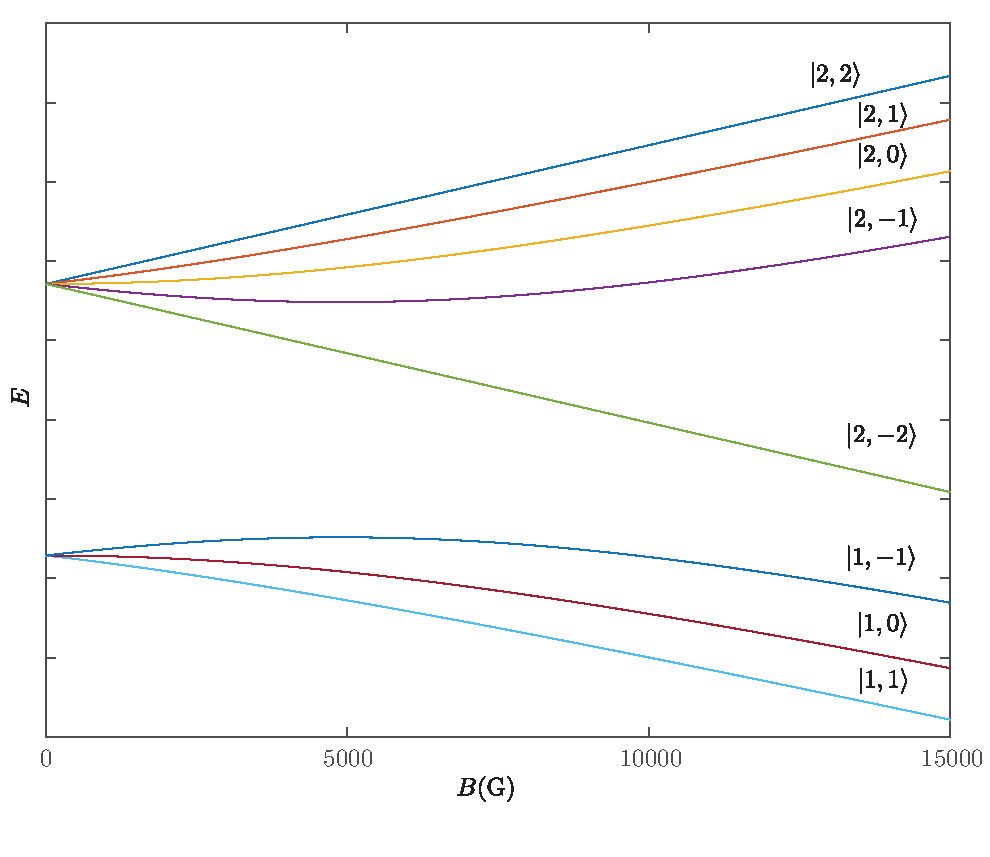
\includegraphics[width=\textwidth]{Chapter2_secs/B_field.pdf}
    \caption{Zeeman splitting of $^{87} {\rm Rb}$ ground states $\ket{F,m_F}$. }
    \label{fig:BField}
\end{figure}

\section{Laser cooling techniques}

\subsection{Two level system interacting with reservoir}

\begin{figure}[htbp]
    \centering
    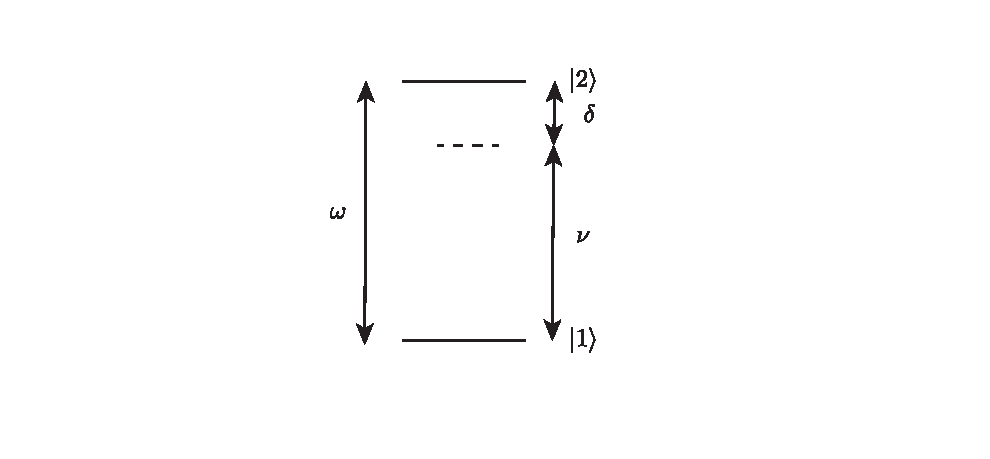
\includegraphics[width=\textwidth]{Chapter2_secs/twolevel.pdf}
    \caption{A two level system with energy difference $\omega$ in a light field with frequency $\nu$. $\delta = \nu - \omega$ is the detuning. }
    \label{fig:twolevel}
\end{figure}
A two level system shown in Fig.~(\ref{fig:twolevel}) interacts with light field via electric dipole interaction. 
\begin{equation}
    \hat{H} = -\Vec{d}\cdot \Vec{E}
\end{equation}
is the electric dipole interaction Hamiltonian where $\Vec{d} = e\Vec{r}$ is the dipole operator. The matrix element of dipole operator $\matrixel{L',m_L'}{\Vec{d}}{L,m_L}$ is nonzero only when $\Delta L = \pm 1$ and $\Delta m_L = 0$. The dipole operator doesn't interact with spin and nuclear angular momentum, so in the total angular momentum basis, the selection rule is 
\begin{equation}
    \Delta F = \pm 1.
\end{equation}
The Electric field
\begin{equation}
    \Vec{E} = E_x {\bf e_x} + E_y {\bf e_y} + E_z {\bf e_z}
\end{equation}
can be expressed in the basis of $\{ {\bf e_{\pm}},{\bf e_z}\}$,
\begin{equation}
    \Vec{E} = E_+ {\bf e_+} + E_- {\bf e_-} + E_z {\bf e_z}.
\end{equation}
Here,
\begin{equation}
    {\bf e_{\pm}} = \frac{{\bf e_x} \pm i{\bf e_y}}{\sqrt{2}}.
\end{equation}
The dipole interaction Hamiltonian is separated into the radial part and the angular part in the new basis,
\begin{equation}
    {\bf e_q}\cdot \Vec{r} = \sqrt{\frac{4\pi}{3}}\rho Y_{1,q}(\theta,\phi),
\end{equation}
here q = 1 for ${\bf e_+}$, q = -1 for ${\bf e_-}$ and q = 0 for ${\bf e_z}$, $Y_{1,q}(\theta,\phi)$ is the spherical harmonic function.

A two level system with energy difference $\omega$ interacts with electromagnetic field
\begin{equation}
    \Vec{E}(\Vec{r},t) = \Vec{E}_0 e^{-i(\nu t-\Vec{k}\cdot\Vec{r})} + \Vec{E}_0^*e^{i(\nu t-\Vec{k}\cdot\Vec{r})},
\end{equation}
the Hamiltonian is
\begin{equation}
    \hat{H} = \hbar \omega \dyad{2}{2} - (\Vec{\mu} \dyad{1}{2} + \Vec{\mu}^*\dyad{2}{1})\cdot\Vec{E}(\Vec{r},t).
\end{equation}
By transforming into a rotating frame, 
\begin{equation}
    \ket{\Tilde{2}} = e^{i\nu t}\ket{2},
\end{equation}
and neglecting the fast oscillating term $e^{\pm i\nu t}$, the Hamiltonian is transformed to
\begin{equation}
    \hat{H} = \hbar\delta \dyad{\Tilde{2}}{\Tilde{2}} + \hbar(\Omega \dyad{1}{\Tilde{2}} + \Omega^* \dyad{\Tilde{2}}{1}),
\end{equation}
Here,
\begin{equation}
    \Omega = \frac{\Vec{E}_0 \cdot \Vec{\mu}}{\hbar}.
\end{equation}
The frame transformation and the removal of the oscillating term is named after rotating wave approximation (RWA), it is widely used in atomic physics when atoms interact with near resonance high frequency optical field, and satisfying the condition $\delta \ll \nu, \omega$.

The Hamiltonian above describes a closed system, where the two level atom only interacts with the one single optical mode and the evolution of atomic states and photon states is coherent. In reality, the atom interacts not only with the optical field but also the vacuum modes in the environment. The vacuum modes are contiguous in free space and discrete in a cavity, the coupling between the atomic states to the vacuum modes leads to spontaneous emission of the excited state and causes incoherence. Wigner-Weisskopf theory \cite{scully1999quantum} represents the vacuum modes with quantized field operators and calculates spontaneous emission with Fermi's golden rule. The Hamiltonian of atomic system and vacuum modes is
\begin{equation}
    \hat{H} = \hbar \omega \dyad{2}{2} + \sum_j\hbar \nu (\hat{a}^\dag_j\hat{a}_j + \frac{1}{2}) - \sum_j(\hbar g_j \dyad{2}{1}\hat{a}_j + \hbar g_j^* \dyad{1}{2}\hat{a}^\dag_j),
\end{equation}
and $g_j$ is the coupling strength between the states $\ket{2,0}$ and $\ket{1,1_k}$. $\ket{1,1_k}$ is the state with one photon occupying mode $k$.
\begin{equation}
    \gamma = 2\pi \sum_j |g_j|^2\delta(\nu_j - \omega)
\end{equation}
is the result of spontaneous emission rate $\gamma$ and in free space
\begin{equation}
    \gamma = \frac{\omega^3|\mu|^2}{3\pi\epsilon_0\hbar c^3},
\end{equation}
which is also known as the Einstein A coefficient.

One way to describe both coherent and incoherent evolution is using density operator. The density operator is defined as
\begin{equation}
    \hat{\rho} = \sum_\alpha p_\alpha \dyad{\phi_\alpha}{\phi_\alpha}.
\end{equation}
Here, $\ket{\phi_\alpha}$ a quantum state and $p_\alpha$ is the probability that the state is in $\ket{\phi_\alpha}$. The states $\ket{\phi_\alpha}$ are not necessarily orthogonal to each other, but for the density operator representation to be valid, it has to satisfy the following condition,
\begin{equation}
    {\rm Tr}[\hat{\rho}] = 1.
\end{equation}
For any orthonormal basis $\{ \ket{n}\}$, 
\begin{equation}
    \sum_n \matrixel{n}{\hat{\rho}}{n} = 1,  and ~ {\rm Tr}[\hat{\rho}] = \sum_n \matrixel{n}{\hat{\rho}}{n},
\end{equation}
for the conservation of probability.

In the density operator representation, the expectation value of a dynamic variable $\hat{A}$ can be calculated using
\begin{equation}
    \expval{\hat{A}} = {\rm \hat{\rho}\hat{A}}.
\end{equation}

In the orthonormal basis $\{ \ket{n}\}$, the matrix element of the density operator is
\begin{equation}
    \rho_{n,n'} = \matrixel{n}{\hat{\rho}}{n'}.
\end{equation}
The diagonal elements $\rho_{n,n}$ represents the the probability that the state is in $\ket{n}$ and the off-diagonal elements $\rho_{n,n'}$ represents the expectation value of coherence between states $\ket{n}$ and $\ket{n'}$. If there exists a state $\ket{\phi}$ such that
\begin{equation}
    \hat{\rho} = \dyad{\phi}{\phi},
\end{equation}
the state represented by $\hat{\rho}$ is a pure state, otherwise, it is a mixed state. In quantum mechanics, the probability amplitude of states bear the full information, probability and coherence. The density operation representation loses the information of coherence of some states but the expectation value of coherence is preserved. 

For an open system, the physical system we are interested in interacts with the environment, or sometimes called reservoir. The reservoir can contain a large number of degrees of freedom, for example, vacuum modes and other electromagnetic fields modes. The large number of degrees of freedom of the reservoir makes it hard to study its dynamics, however, in many cases, we are not actually interested in learning about the evolution of the reservoir. In these cases, it is useful to ignore the dynamics of the reservoir and only keep the effect the reservoir has on the system. By making this assumption, the coherent evolution of the system and the reservoir is lost and there exists decoherence in the dynamic of the system, so density operator is widely used to describe the open system.

The full Hamiltonian is
\begin{equation}
    \hat{H} = \hat{H}_S +\hat{H}_R + \hat{H}_{SR} 
\end{equation}
and under Heisenberg's equation, the evolution of the density operator is
\begin{equation}
    \frac{d}{dt}\hat{\rho} = \frac{1}{i\hbar}\left[ \hat{H},\hat{\rho} \right]
\end{equation}
Assume the interaction operator takes the form
\begin{equation}
    \hat{H}_{SR}  = \hat{S}\hat{R}^\dag + \hat{S}^\dag\hat{R}.
\end{equation}
To ignore the dynamics of the reservoir and only keep the effects it has on the system, we need to make two assumptions. First, factorize the reservoir operator
\begin{equation}
    \hat{R} \approx f(t)\hat{\Tilde{R}}.
\end{equation}
The function $f(t)$ characterizes the time evolution of the reservoir, and it is often assumed that the reservoir is stationary in the stochastic process language. The auto-correlation function of $f(t)$ is defined as
\begin{equation}
    ACF_f(t-t') = \expval{(f(t)-\expval{f(t)})(f(t')-\expval{f(t')})}.
\end{equation}
The correlation time $t_c$ of the function $f(t)$ is defined as the width of the peak of $ACF_f(t-t')$. 
The first assumption of reservoir is that $t_c \ll 1$, which means the reservoir has Markovian property, it quickly forgets about its previous state does not keep the memory of interacting with the system.

The second assumption is the reservoir is large enough that the system can hardly affect its state. Again, this means that the reservoir is stationary. Under these assumptions, the dynamics of the system is derived and expressed in terms of the reduced density operator
\begin{equation}
    \hat{\rho}_S = {\rm Tr}_{\rm R} [\hat{\rho}],
\end{equation}
which takes the average of the reservoir state by tracing out the reservoir degrees of freedom.

For a two level system
\begin{equation}
    \hat{H}_S = \hbar\delta \dyad{2}{2} + \hbar(\Omega \dyad{1}{2} + \Omega^* \dyad{2}{1}),
\end{equation}
the density operator evolves under eqaution
\begin{align}\label{OBE}
    &\dot{\rho}_{22} = -\gamma(\overline{n} + 1)\rho_{22} + \gamma\overline{n}\rho_{11} + i\Omega^*\rho_{21} - i\Omega\rho_{12}\\\nonumber
    &\dot{\rho}_{11} = \gamma(\overline{n} + 1)\rho_{22} - \gamma\overline{n}\rho_{11} - i\Omega^*\rho_{21} + i\Omega\rho_{12}\\\nonumber
    &\dot{\rho}_{12} = -\frac{\gamma}{2}(2\overline{n} + 1)\rho_{12} - i\delta\rho_{12} - i\Omega^*(\rho_{22}-\rho_{11})\\\nonumber
    &\dot{\rho}_{21} = -\frac{\gamma}{2}(2\overline{n} + 1)\rho_{21} + i\delta\rho_{21} + i\Omega(\rho_{22}-\rho_{11})\\\nonumber
\end{align}
This is known as the {\bf Optical Bloch equations}, and also called \textbf{Master equation} \cite{metcalf2007laser}. The first two equations describe the evolution of the probability of occupying the states $\ket{2}$ and $\ket{1}$.  The third and fourth equations describe the evolution of expected coherence between states $\ket{1}$ and $\ket{2}$. The term $\gamma(\overline{n} + 1)\rho_{22}$ combines spontaneous emission ($\gamma\rho_{22}$) and stimulated emission ($\gamma\overline{n}\rho_{22}$). 


\subsection{Optical force}
An atomic system interacts with optical fields, which leads to stimulated emission and Rabi oscillation when the frequency of the field is near resonance. When the field is far-detuned, the atoms see a spin-independent spatial potential, the force of which drives the atoms' center-of-mass motion. Also, the atoms interact with the vacuum modes that lead to spontaneous emission. The emitted photons have nonzero momentum, so the atoms acquire the recoil momentum when the spontaneous emission happens. From the classical physics point of view, the atoms should experience a "force" in the optical fields and the definition of the "force" can be borrowed from classical physics.
\begin{equation}
    \hat{F} = \frac{d}{dt}\hat{p} = \frac{1}{ih}[\hat{p},\hat{H}]
\end{equation}
The same as classical physics, the force operator is defined as the rate of momentum change and it can be calculated for a two-level atomic system with Hamiltonian
\begin{equation}
    \hat{H} = \hbar\delta \dyad{2}{2} + \hbar(\Omega(\Vec{r}) \dyad{1}{2} + \Omega^*(\Vec{r}) \dyad{2}{1}).
\end{equation}
$\Omega(\Vec{r})$ is a function of $\Vec{r}$ for the inhomogeneous field amplitude. 
\begin{equation}
    \Vec{F} = -[\nabla,\Vec{H}(\Vec{r})] = \hbar\nabla\Omega(\Vec{r})\dyad{2}{1} + \hbar\nabla\Omega^*(\Vec{r})\dyad{1}{2}
\end{equation}
The state of the system is represented by density operator $\hat{\rho}$ and the expectation value of operator $\hat{F}$ is
\begin{align}
    \expval{\hat{F}} &= {\rm Tr}[\hat{\rho}\hat{F}]\\ \nonumber
    &=\hbar\nabla\Omega\rho_{12} + \hbar\nabla\Omega^*\rho_{21}\\\nonumber
    &=2\hbar|\Omega|^2\nabla\phi{\rm Im}\left( \frac{\rho_{21}}{\Omega}\right) + \hbar\nabla|\Omega|^2{\rm Re}\left( \frac{\rho_{21}}{\Omega}\right)\\\nonumber
\end{align}
Here, $\phi$ is the phase of the field,
\begin{equation}
    \Omega = |\Omega|e^{i\phi}.
\end{equation}
The first term is interpreted as the dissipative force and the second term the reactive force. This can be more intuitively understood when we look at the form of the force in two extreme cases.

For the steady solution of the optical Bloch equation,
\begin{align}
    &\rho_{21} = \frac{i\Omega(\rho_{22}-\rho_{11})}{\gamma_{21} - i\delta}\\\nonumber
    &\rho_{22} = \frac{R}{\gamma(\overline{n} + 1) + 2R}\\\nonumber
    &R = \frac{2\gamma_{21}|\Omega|^2}{\gamma_{21}^2 + \delta^2}\\\nonumber
\end{align}
here, $\gamma_{21}$ is the decay rate of coherence and $R$ is the optical pumping rate, the rate the atoms are pumped from the ground state to the excited state. When the field is weak,
\begin{equation}
    |\Omega| \ll \gamma
\end{equation}
the time atoms spend in the excited state is close to zero, $\rho_{22} \approx 0$. The coherence $\rho_{21}$ can be approximated with
\begin{equation}
    \rho_{21} = \Omega\frac{\delta - i\gamma_{21}}{\gamma_{21}^2 + \delta^2}
\end{equation}
The dissipative force takes the form
\begin{align}
    F_{dis} &= 2\hbar|\Omega|^2 \Vec{k}\frac{\gamma_{21}}{\gamma_{21}^2 + \delta^2}\\\nonumber
    &= \hbar\Vec{k}R\\
\end{align}
Intuitively, it means every time the atom is pumped from the ground state to the excited state, it acquires momentum $\hbar\Vec{k}$. When spontaneous emission happens, the photon is emitted in any direction with equal probability, on the average, the atom does not acquire momentum in spontaneous emission. 

In the other case, when $\delta$ is large, 
\begin{equation}
    \delta \gg |\Omega|, \delta \gg \gamma_{21}    
\end{equation}
Optical pumping rate $R \approx 0$ and the population in the excited state $\rho_{22} \approx 0$. 
\begin{equation}
    {\rm Im}\left[\frac{\rho_{21}}{\Omega}\right] \approx \frac{1}{\delta}
\end{equation}
and the reactive force takes the form
\begin{equation}
    F_{react} = \frac{\hbar\nabla|\Omega|^2}{\delta}.
\end{equation}
Effectively, the atoms see a potential
\begin{equation}
    V(\Vec{r}) = -\frac{\hbar|\Omega(\Vec{r})|^2}{\delta}
\end{equation}
The potential is spin-independent, its strength is proportional to the intensity of the field $|\Omega\Vec{r}|^2$ and the sign of $\delta$ determines if the potential is repulsive or attractive. When $\delta > 0$, the field is red detuned, and the potential is lower for stronger intensity, so the potential is attractive. When the field is blue detuned, it is repulsive.  

This potential is known as the dipole potential, it originates from the AC stark shift. Due to the large detuning, it does not drive the transition of internal states but changes the energy of the ground state so it is effectively a spin-independent potential. Dipole potential is widely used in atomic physics experiments. It can be used as an attractive trap, called a dipole trap, to trap atoms, to do evaporative cooling, and to make an optical lattice. 
The repulsive potential is also very useful, it can be used to make a 1D trap when the laser is in Laguerre-Gaussian mode \cite{salces2018equations} and make random repulsive potential (optical speckle) which is discussed in detail in Ch.~(\ref{speckle_chapter}).

    


\titleformat{\chapter}
{\normalfont\large}{Appendix \thechapter:}{1em}{}
\appendix
\section{Postulates of Quantum Mechanics}
\label{appendix:QMP}
1.At each instant the state of a physical system is represented by $\ket{\psi}$ in the space of
states.

2.Every observable attribute of a physical system is described by an operator that acts on the
kets that describe the system.

3.The only possible result of the measurement of an observable $A$ is one of the eigenvalues of
the corresponding operator $\hat{\mathcal{A}}$.

4.When a measurement of an observable $\mathcal{A}$ is made on a generic state $\ket{\psi}$, the probability
of obtaining an eigenvalue an is given by the square of the inner product of $\ket{\psi}$ with the
eigenstate $\ket{a_n}$, $|\bra{a_n}\ket{\psi}|^2$.

5.Immediately after the measurement of an observable $\mathcal{A}$ has yielded a value $a_n$, the state of
the system is the normalized eigenstate $\ket{a_n}$.

6.The time evolution of a quantum system preserves the normalization of the associated ket.
The time evolution of the state of a quantum system is described by 
\begin{equation}
    i\hbar\frac{d}{dt}\ket{\psi(t)} = \mathcal{H}\ket{\psi(t)}
\end{equation}



\appendix
\renewcommand{\thechapter}{A}
\chapter{Calculation results of field-field correlation function}
\label{appendix:CF}

For field-field correlation function, in the free propagation case, the original calculation results are:

\begin{align}
\frac{C_E({\bf r}_1,{\bf r}_2;z)}{E_0^2} =& \left[\frac{w}{w(z)}\right]^2 \exp(-ik_0\frac{{\bf r}_1^2 - {\bf r}_2^2}{2 R(z)})\\
&\times \exp(-\frac{{\bf r}_1^2 + {\bf r}_2^2}{w(z)^2})\exp(-\frac{|{\bf r}_1-{\bf r}_2|^2}{\sigma(z)^2}) \nonumber 
\end{align}

\begin{equation}
    \begin{cases}
    %&{\bf \bar{r}}=({\bf r_1}+{\bf r_2})/2\\
    &1/R(z) = 1/z - k_0^2w^2/8Az^3\\
    &1/\sigma^2(z)=k_0^2w^2/8z^2 - k_0^4w^4/64Az^4 - k_0^2/16Az^2\\
    &1/w^2(z) = k_0^2/8Az^2\\
    &A = 1/2w^2 + 1/\sigma^2 + k_0^2w^2/8z^2
    \end{cases}
\end{equation}

With a lens, 
\begin{align}
\frac{C_E({\bf r}_1,{\bf r}_2;z)}{E_0^2} =& \frac{k_0^2w^2}{4z^2D} \exp\left[-i\left(\frac{k_0}{2z} + \frac{z_L^2AB}{2Dz^2}\right)({\bf r}_1^2 - {\bf r}_2^2)\right]\\
&\times \exp\left[-\frac{k_0^2({\bf r}_1^2 + {\bf r}_2^2)}{4z^2D}\right]\exp\left[-\left( \frac{z_L^2A}{2z^2} -\frac{z_L^4A^2B^2}{2k_0^2z^2D} - \frac{k_0^2}{8z^2D}\right)|{\bf r}_1-{\bf r}_2|^2\right] \nonumber 
\end{align}
where,
\begin{equation}
    \begin{cases}
    &A = 1/2w^2 + 1/\sigma^2 + k_0^2w^2/8z_L^2\\
    &B = \frac{k_0^3w^2}{8z_L^3A} - k_0(1/z+1/z_L-1/f)\\
    &C = \frac{k_0^2w^2}{8z_L^2} - \frac{k_0^4w^4}{64z_L^4A}\\
    &D = \frac{z_L^2AB^2}{k_0^2} + C\\
    \end{cases}
\end{equation}
\appendix
\renewcommand{\thechapter}{C}
\chapter{Derivation of the moments of random phase factors}
\label{appendix:moments}

In Sec.~\ref{prob sec}, we derive the joint probability density of random electric fields and the probability density of intensity \ref{P of int} by calculating the moments of the random electric fields. Under our assumptions in Sec.~\ref{prob sec}, the moments of the random electric fields are proportional the moments of the random phase factors $\phi({\bf r}')$.

Under assumptions:

\begin{align}\label{gaussian C_E}
\langle \exp\left\{- i \left[\phi({\bf r}_1)-\phi({\bf r}_2)\right]\right\}\rangle &= \exp(-\frac{|{\bf r}_1-{\bf r}_2|^2}{\sigma^2}), 
\end{align} 

and

\begin{equation}
    \phi({\bf r}) \sim Uniform(0,2\pi).
\end{equation}

\begin{align}\label{gaussian C_E}
\langle \exp\left\{- i \left[\phi({\bf r}_1)-\phi({\bf r}_2)\right]\right\}\rangle &= \langle \cos\left[\phi({\bf r}_1)-\phi({\bf r}_2)\right] - i\sin\left[\phi({\bf r}_1)-\phi({\bf r}_2)\right]\rangle \\\nonumber
&=\langle \cos\left[\phi({\bf r}_1)-\phi({\bf r}_2)\right]\rangle - i\langle\sin\left[\phi({\bf r}_1)-\phi({\bf r}_2)\right]\rangle\\\nonumber
\end{align}

By symmetry,
\begin{equation}
    \langle\sin\left[\phi({\bf r}_1)-\phi({\bf r}_2)\right]\rangle = \langle\sin\left[\phi({\bf r}_2)-\phi({\bf r}_1)\right]\rangle = 0,
\end{equation}
therefore,
\begin{equation}
    \langle \cos\left[\phi({\bf r}_1)-\phi({\bf r}_2)\right]\rangle = \exp(-\frac{|{\bf r}_1-{\bf r}_2|^2}{\sigma^2}).
\end{equation}

\begin{align}
    \langle \cos\left[\phi({\bf r}_1)+\phi({\bf r}_2)\right]\rangle &=\langle \cos\left[\phi({\bf r}_1)-\phi({\bf r}_2) + 2\phi({\bf r}_2)\right]\rangle\\\nonumber
    &=  \langle \cos\left[\phi({\bf r}_1)-\phi({\bf r}_2)\right]\cos\left[2\phi({\bf r}_2)\right]\rangle\\\nonumber
    & -\langle \sin\left[\phi({\bf r}_1)-\phi({\bf r}_2)\right]\sin\left[2\phi({\bf r}_2)\right]\rangle\\\nonumber
\end{align}
$\phi({\bf r}_1)-\phi({\bf r}_2)$ is independent of $\phi({\bf r}_2)$, so
\begin{equation}
    \langle \cos\left[\phi({\bf r}_1)+\phi({\bf r}_2)\right]\rangle = 0
\end{equation}

Similarly,
\begin{equation}
    \langle \sin\left[\phi({\bf r}_1)+\phi({\bf r}_2)\right]\rangle = 0
\end{equation}

\begin{align}
    \langle \cos\left[\phi({\bf r}_1)\right]\cos\left[\phi({\bf r}_2)\right]\rangle &=\frac{1}{2}\langle \cos\left[\phi({\bf r}_1)+\phi({\bf r}_2)\right] + \cos\left[\phi({\bf r}_1)-\phi({\bf r}_2)\right]\rangle\\\nonumber
    & = \frac{1}{2}\exp(-\frac{|{\bf r}_1-{\bf r}_2|^2}{\sigma^2})\\\nonumber
\end{align}

\begin{align}
    \langle \sin\left[\phi({\bf r}_1)\right]\sin\left[\phi({\bf r}_2)\right]\rangle &=\frac{1}{2}\langle \cos\left[\phi({\bf r}_1)-\phi({\bf r}_2)\right] - \cos\left[\phi({\bf r}_1)+\phi({\bf r}_2)\right]\rangle\\\nonumber
    & = \frac{1}{2}\exp(-\frac{|{\bf r}_1-{\bf r}_2|^2}{\sigma^2})\\\nonumber
\end{align}

\begin{align}
    \langle \sin\left[\phi({\bf r}_1)\right]\cos\left[\phi({\bf r}_2)\right]\rangle &=\frac{1}{2}\langle \sin\left[\phi({\bf r}_1)+\phi({\bf r}_2)\right] - \sin\left[\phi({\bf r}_1)-\phi({\bf r}_2)\right]\rangle\\\nonumber
    & = 0\\\nonumber
\end{align}

\begin{align}
    \langle \cos\left[\phi({\bf r}_1)\right]\sin\left[\phi({\bf r}_2)\right]\rangle &=\frac{1}{2}\langle \sin\left[\phi({\bf r}_1)+\phi({\bf r}_2)\right] - \sin\left[\phi({\bf r}_2)-\phi({\bf r}_1)\right]\rangle\\\nonumber
    & = 0\\\nonumber
\end{align}
\appendix
\renewcommand{\thechapter}{C}
\chapter{Squared coupling strength between momentum states}
\label{appendix:squared_coupling}

In Sec.~\ref{sec_spinless_atoms}, we stated this formula 
\begin{equation}
    \rho(k_f-k_0) = \langle\bra{k_f}\hat V\ket{k_0}\bra{k_0}\hat V\ket{k_f}\rangle
\end{equation}
and applied it in the Fermi's golden rule calculation. Here we derive it.

In the basis of momentum states $\{\ket{k}\}$, the matrix element of speckle potential $\hat{V}(x)$ is 

\begin{equation}
    g(k_1,k_2) = \matrixel{k_1}{\hat{V}(x)}{k_2}.
\end{equation}
The ensemble averaged, squared matrix elements is

\begin{align}
    \langle |g(k_1,k_2)|^2 \rangle &= \langle \matrixel{k_1}{\hat{V}(x)}{k_2}\matrixel{k_2}{\hat{V}(x)}{k_1} \rangle\\\nonumber
    & = \langle \frac{1}{\sqrt{2\pi}}\int V(x_1)\exp{i(k_0-k_1)x_1} dx_1 \frac{1}{\sqrt{2\pi}}\int  V(x_2)\exp{-i(k_0-k_1)x_2} dx_2 \rangle\\\nonumber
    & = \frac{1}{2\pi}\iint \langle V(x_1)V(x_2)\rangle\exp{-i\Delta k(x_1-x_2)}dx_1dx_2\\\nonumber
    & = \rho_V(\Delta k)\\\nonumber
\end{align}

Here $\rho_V(\Delta k)$ is the PSD of the speckle potential and $\Delta k = k_2-k_1$. Since speckle potential is proportional to the intensity of optical speckle, 
\begin{equation}
    \rho_V(\Delta k) \propto \rho_I(\Delta k)  
\end{equation}
\appendix
\renewcommand{\thechapter}{C}
\chapter{Speckle beam width in the focal plane from a ray optics model}
\label{appendix:beam_width}

The speckle beam width in the focal plane of a lens can be calculated from a ray optics model, in the limit of large focal length $f$ and small diverging angle $\Delta \theta$.

\begin{figure}[htbp]
    \centering
    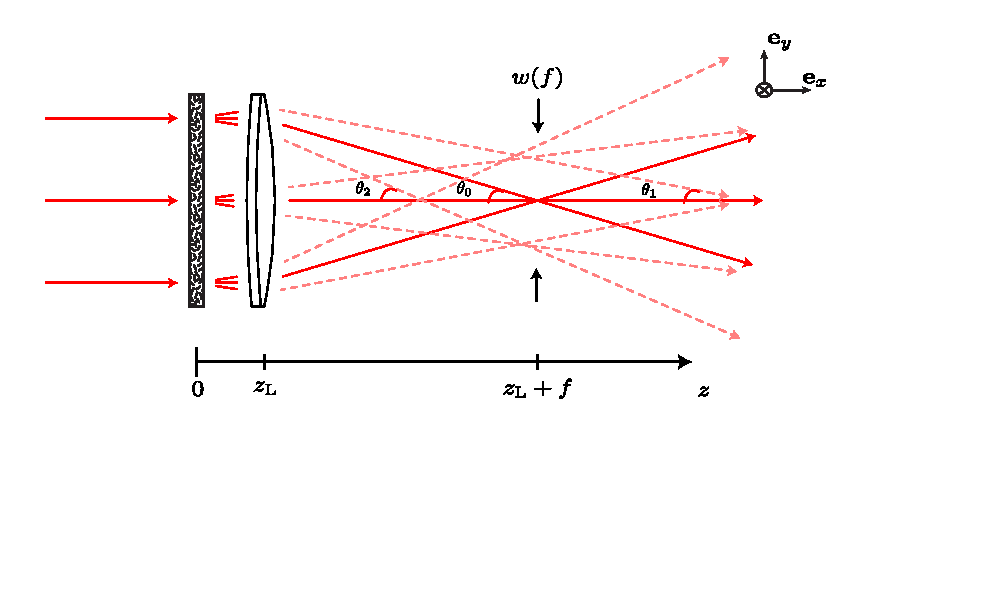
\includegraphics[width=\textwidth]{Fig1_appen.pdf}
    \caption{A ray optics model to calculate the speckle beam width in the focal plane of a lens.}
    \label{fig:append1}
\end{figure}

As shown in Fig.~\ref{fig:append1}, an optical ray hit the edge of a lens is focused to the focal point and form an angle $theta_0$ with $x$-axis. After the phase plate the speckle beam diverges at an angle $\Delta \theta$, and the diverged beam form angles $\theta_1$ and $theta_2$ with the $x$-axis.

\begin{align}
    \theta_1 &\approx \theta_0 - \Delta \theta\\\nonumber
    \theta_2 &\approx \theta_0 + \Delta \theta\\\nonumber
    f &= \frac{D_L}{2\tan{\theta_0}}\\\nonumber
\end{align}

For small $\Delta \theta$,
\begin{align}
    w(f) &= D_L \frac{\tan{\theta_2}-\tan{\theta_1}}{\tan{\theta_2}+\tan{\theta_1}}\\\nonumber
    & \approx D_L \frac{\sec{\theta_0}^2 \Delta \theta}{\tan{\theta_0}}\\\nonumber
    & = \frac{D_L\Delta \theta}{\sin{\theta_0}\cos{\theta_0}}\\\nonumber
\end{align}

In the limit of large $f$, $\sin{\theta_0} \approx \frac{D_L}{2f}$, $\cos{\theta_0} \approx 1$.
\begin{equation}
    w(f) \approx 2f\Delta \theta.
\end{equation}


\renewcommand{\baselinestretch}{1}
\small\normalsize
%\include{Bibliography} %Delete this line if using Bibtex or Natbib

%When using Bibtex, delete the previous line and use the following
%three lines:
\newpage
\bibliographystyle{unsrt}
\bibliography{1References} %replace "Galactic,Dottie" with the
%                 file name(s) of your bib file(s)

%When using Natbib, use the following three lines:
%\newpage
%\bibliographystyle{unsrtnat}
%bibliography{Galactic,Dottie} %replace "Galactic,Dottie" with the
%                 file name(s) of your bib file(s)

\end{document}
